% Options for packages loaded elsewhere
\PassOptionsToPackage{unicode}{hyperref}
\PassOptionsToPackage{hyphens}{url}
\PassOptionsToPackage{dvipsnames,svgnames,x11names}{xcolor}
%
\documentclass[
  letterpaper,
  DIV=11,
  numbers=noendperiod]{scrreprt}

\usepackage{amsmath,amssymb}
\usepackage{iftex}
\ifPDFTeX
  \usepackage[T1]{fontenc}
  \usepackage[utf8]{inputenc}
  \usepackage{textcomp} % provide euro and other symbols
\else % if luatex or xetex
  \usepackage{unicode-math}
  \defaultfontfeatures{Scale=MatchLowercase}
  \defaultfontfeatures[\rmfamily]{Ligatures=TeX,Scale=1}
\fi
\usepackage{lmodern}
\ifPDFTeX\else  
    % xetex/luatex font selection
\fi
% Use upquote if available, for straight quotes in verbatim environments
\IfFileExists{upquote.sty}{\usepackage{upquote}}{}
\IfFileExists{microtype.sty}{% use microtype if available
  \usepackage[]{microtype}
  \UseMicrotypeSet[protrusion]{basicmath} % disable protrusion for tt fonts
}{}
\makeatletter
\@ifundefined{KOMAClassName}{% if non-KOMA class
  \IfFileExists{parskip.sty}{%
    \usepackage{parskip}
  }{% else
    \setlength{\parindent}{0pt}
    \setlength{\parskip}{6pt plus 2pt minus 1pt}}
}{% if KOMA class
  \KOMAoptions{parskip=half}}
\makeatother
\usepackage{xcolor}
\setlength{\emergencystretch}{3em} % prevent overfull lines
\setcounter{secnumdepth}{5}
% Make \paragraph and \subparagraph free-standing
\makeatletter
\ifx\paragraph\undefined\else
  \let\oldparagraph\paragraph
  \renewcommand{\paragraph}{
    \@ifstar
      \xxxParagraphStar
      \xxxParagraphNoStar
  }
  \newcommand{\xxxParagraphStar}[1]{\oldparagraph*{#1}\mbox{}}
  \newcommand{\xxxParagraphNoStar}[1]{\oldparagraph{#1}\mbox{}}
\fi
\ifx\subparagraph\undefined\else
  \let\oldsubparagraph\subparagraph
  \renewcommand{\subparagraph}{
    \@ifstar
      \xxxSubParagraphStar
      \xxxSubParagraphNoStar
  }
  \newcommand{\xxxSubParagraphStar}[1]{\oldsubparagraph*{#1}\mbox{}}
  \newcommand{\xxxSubParagraphNoStar}[1]{\oldsubparagraph{#1}\mbox{}}
\fi
\makeatother


\providecommand{\tightlist}{%
  \setlength{\itemsep}{0pt}\setlength{\parskip}{0pt}}\usepackage{longtable,booktabs,array}
\usepackage{calc} % for calculating minipage widths
% Correct order of tables after \paragraph or \subparagraph
\usepackage{etoolbox}
\makeatletter
\patchcmd\longtable{\par}{\if@noskipsec\mbox{}\fi\par}{}{}
\makeatother
% Allow footnotes in longtable head/foot
\IfFileExists{footnotehyper.sty}{\usepackage{footnotehyper}}{\usepackage{footnote}}
\makesavenoteenv{longtable}
\usepackage{graphicx}
\makeatletter
\def\maxwidth{\ifdim\Gin@nat@width>\linewidth\linewidth\else\Gin@nat@width\fi}
\def\maxheight{\ifdim\Gin@nat@height>\textheight\textheight\else\Gin@nat@height\fi}
\makeatother
% Scale images if necessary, so that they will not overflow the page
% margins by default, and it is still possible to overwrite the defaults
% using explicit options in \includegraphics[width, height, ...]{}
\setkeys{Gin}{width=\maxwidth,height=\maxheight,keepaspectratio}
% Set default figure placement to htbp
\makeatletter
\def\fps@figure{htbp}
\makeatother
% definitions for citeproc citations
\NewDocumentCommand\citeproctext{}{}
\NewDocumentCommand\citeproc{mm}{%
  \begingroup\def\citeproctext{#2}\cite{#1}\endgroup}
\makeatletter
 % allow citations to break across lines
 \let\@cite@ofmt\@firstofone
 % avoid brackets around text for \cite:
 \def\@biblabel#1{}
 \def\@cite#1#2{{#1\if@tempswa , #2\fi}}
\makeatother
\newlength{\cslhangindent}
\setlength{\cslhangindent}{1.5em}
\newlength{\csllabelwidth}
\setlength{\csllabelwidth}{3em}
\newenvironment{CSLReferences}[2] % #1 hanging-indent, #2 entry-spacing
 {\begin{list}{}{%
  \setlength{\itemindent}{0pt}
  \setlength{\leftmargin}{0pt}
  \setlength{\parsep}{0pt}
  % turn on hanging indent if param 1 is 1
  \ifodd #1
   \setlength{\leftmargin}{\cslhangindent}
   \setlength{\itemindent}{-1\cslhangindent}
  \fi
  % set entry spacing
  \setlength{\itemsep}{#2\baselineskip}}}
 {\end{list}}
\usepackage{calc}
\newcommand{\CSLBlock}[1]{\hfill\break\parbox[t]{\linewidth}{\strut\ignorespaces#1\strut}}
\newcommand{\CSLLeftMargin}[1]{\parbox[t]{\csllabelwidth}{\strut#1\strut}}
\newcommand{\CSLRightInline}[1]{\parbox[t]{\linewidth - \csllabelwidth}{\strut#1\strut}}
\newcommand{\CSLIndent}[1]{\hspace{\cslhangindent}#1}

\usepackage{fontspec}
\usepackage{multirow}
\usepackage{multicol}
\usepackage{colortbl}
\usepackage{hhline}
\newlength\Oldarrayrulewidth
\newlength\Oldtabcolsep
\usepackage{longtable}
\usepackage{array}
\usepackage{hyperref}
\usepackage{float}
\usepackage{wrapfig}
\KOMAoption{captions}{tableheading}
\makeatletter
\@ifpackageloaded{bookmark}{}{\usepackage{bookmark}}
\makeatother
\makeatletter
\@ifpackageloaded{caption}{}{\usepackage{caption}}
\AtBeginDocument{%
\ifdefined\contentsname
  \renewcommand*\contentsname{Table of contents}
\else
  \newcommand\contentsname{Table of contents}
\fi
\ifdefined\listfigurename
  \renewcommand*\listfigurename{List of Figures}
\else
  \newcommand\listfigurename{List of Figures}
\fi
\ifdefined\listtablename
  \renewcommand*\listtablename{List of Tables}
\else
  \newcommand\listtablename{List of Tables}
\fi
\ifdefined\figurename
  \renewcommand*\figurename{Figure}
\else
  \newcommand\figurename{Figure}
\fi
\ifdefined\tablename
  \renewcommand*\tablename{Table}
\else
  \newcommand\tablename{Table}
\fi
}
\@ifpackageloaded{float}{}{\usepackage{float}}
\floatstyle{ruled}
\@ifundefined{c@chapter}{\newfloat{codelisting}{h}{lop}}{\newfloat{codelisting}{h}{lop}[chapter]}
\floatname{codelisting}{Listing}
\newcommand*\listoflistings{\listof{codelisting}{List of Listings}}
\makeatother
\makeatletter
\makeatother
\makeatletter
\@ifpackageloaded{caption}{}{\usepackage{caption}}
\@ifpackageloaded{subcaption}{}{\usepackage{subcaption}}
\makeatother

\ifLuaTeX
  \usepackage{selnolig}  % disable illegal ligatures
\fi
\usepackage{bookmark}

\IfFileExists{xurl.sty}{\usepackage{xurl}}{} % add URL line breaks if available
\urlstyle{same} % disable monospaced font for URLs
\hypersetup{
  pdftitle={Quesnel-Bowron Watershed Connectivity Remediation Plan: 2024 - },
  pdfauthor={Canadian Wildlife Federation},
  colorlinks=true,
  linkcolor={blue},
  filecolor={Maroon},
  citecolor={Blue},
  urlcolor={Blue},
  pdfcreator={LaTeX via pandoc}}


\title{Quesnel-Bowron Watershed Connectivity Remediation Plan: 2024 -}
\author{Canadian Wildlife Federation}
\date{29-11-2024}

\begin{document}
\maketitle

\renewcommand*\contentsname{Table of contents}
{
\hypersetup{linkcolor=}
\setcounter{tocdepth}{1}
\tableofcontents
}

\bookmarksetup{startatroot}

\chapter*{Acknowledgements}\label{acknowledgements}
\addcontentsline{toc}{chapter}{Acknowledgements}

\markboth{Acknowledgements}{Acknowledgements}

\includegraphics{spawn.jpg}

\bookmarksetup{startatroot}

\chapter*{Project Overview}\label{project-overview}
\addcontentsline{toc}{chapter}{Project Overview}

\markboth{Project Overview}{Project Overview}

\section*{Connectivity Plan Purpose and
Approach}\label{connectivity-plan-purpose-and-approach}
\addcontentsline{toc}{section}{Connectivity Plan Purpose and Approach}

\markright{Connectivity Plan Purpose and Approach}

SAMPLE The following Watershed Connectivity Remediation Plan (WCRP)
represents the culmination of a one-year collaborative planning effort
for the Bulkley River watershed (excluding the Morice River, see Project
Scope), the overall aim of which is to clarify and reduce the threat of
aquatic barriers to anadromous salmonids and the livelihoods that they
support, including the values and laws of First Nations, as well their
continued sustenance, cultural, and ceremonial needs both now and into
the future. This 10-year plan was developed to identify priority actions
that the Bulkley River WCRP planning team (see Table~\ref{tbl-planteam}
for a list of team members) will undertake between 2021-2031 to conserve
and restore fish passage in the watershed through strategies aimed at
barrier remediation, barrier prevention, and strengthening Indigenous
connections to land and water.

WCRPs are long-term, actionable plans that blend local stakeholder and
rightsholder knowledge with innovative GIS analyses to gain a shared
understanding of where remediation efforts will have the greatest
benefit for anadromous salmonids. The planning process is inspired by
the
\href{https://cmp-openstandards.org/wp-content/uploads/2020/07/CMP-Open-Standards-for-the-Practice-of-Conservation-v4.0.pdf}{Conservation
Standards} (v.4.0), which is a conservation planning framework that
allows planning teams to systematically identify, implement, and monitor
strategies to apply the most effective solutions to high priority
conservation problems. There is a rich history of connectivity and fish
passage planning and remediation work in the Bulkley River watershed
that this WCRP builds upon, including the work undertaken by the BC Fish
Passage Technical Working Group, the Skeena Fisheries Commission, the
Office of the Wet'suwet'en, the Wet'suwet'en First Nation, and the
Society for Ecosystem Restoration in Northern British Columbia (SERNbc)
among others ((\textbf{Wilson2007?}), (\textbf{Mccarthy2015?}),
(\textbf{Smith2018?}), (\textbf{Casselman?}), (\textbf{Irvine2018?})).
The Canadian Wildlife Federation will continue to engage and coordinate
with local partners and existing initiatives, in part through the Skeena
Environmental Stewardship Initiative. SERNbc is also currently
undertaking undertaking
\href{https://www.newgraphenvironment.com/fish_passage_bulkley_2020_reporting/Bulkley.pdf}{fish
passage} work in the Bulkley River watershed, with some overlap and some
differences in scope compared to the work and processes described in
this WCRP. The SERNbc project relies on expert knowledge and field
assessments in both the Bulkley and Morice watersheds to improve passage
for all fish, including fluvial and resident species, and focuses on
stream crossings that act as barriers ((\textbf{Irvine2021?})). This
WCRP focuses specifically on improving connectivity for anadromous
salmonid species and uses consensus-based planning exercises and spatial
model implementation to develop watershed-scale status assessments, goal
setting, and prioritization for multiple barrier types. SERNbc and the
WCRP planning team are currently collaborating on the development of the
\href{https://github.com/smnorris/bcfishpass}{bcfishpass} connectivity
model and will continue to work together to promote coordination and
collaboration between the two initiatives moving forward.

The planning team compiled existing barrier location and assessment
data, habitat data, and previously identified priorities, and combined
this with local and Indigenous knowledge to create a strategic
watershed-scale plan to improve connectivity. To expand on this work,
the Bulkley River WCRP planning team applied the WCRP planning framework
to define the ``thematic'' scope of freshwater connectivity and refine
the ``geographic'' scope to identify those portions of the watershed
where barrier prioritization will be conducted, and subsequent
remediation efforts will take place. Additionally, the team selected
target fish species, assessed their current connectivity status in the
watershed, defined concrete goals for gains in connectivity, and
developed a priority list of barriers for remediation to achieve those
goals. During the 2021 field season, 28 barrier assessments and 21
habitat confirmations were completed. Seventeen barriers were added to
the intermediate barrier list based on 2021 field assessments, and an
additional 17 crossings were removed from the list, due to being
passable, not existing, or having low quality habitat (see
\textbf{?@tbl-removed-from-consideration}). The preliminary barriers
list was further divided this year into an ``intermediate barriers''
list (see \textbf{?@tbl-intermediate}), which includes barriers that
require further assessment, and a ``priority barriers'' list (see
Table~\ref{tbl-priority}), which includes barriers that are actively
being pursued for design and remediation. While the current version of
this plan is based on the best-available information at the time of
publishing, WCRPs are intended to be ``living plans'' that are updated
regularly as new information becomes available, or if local priorities
and contexts change. As such, this document should be interpreted as a
current ``snap-shot'' in time, and future iterations of this WCRP will
build upon the material presented in this plan to continuously improve
aquatic barrier remediation for migratory fish in the Bulkley River
watershed. For more information on how WCRPs are developed, see
Mazany-Wright, Noseworthy, et al. (2021).

\section*{Vision Statement}\label{vision-statement}
\addcontentsline{toc}{section}{Vision Statement}

\markright{Vision Statement}

SAMPLE Healthy, well-connected streams and rivers within the Bulkley
River watershed support thriving populations of migratory and resident
fish. In turn, these fish provide the continued sustenance, cultural,
and ceremonial needs of the Wet'suwet'en and Gitxsan peoples, as they
have since time immemorial. First Nations, residents, and visitors to
the watershed work together for environmental stewardship to clarify,
implement, and assess the effectiveness of actions to mitigate the
negative effects of aquatic barriers, improving the resiliency of
streams and rivers for the benefit and appreciation of all.

\section*{Project Scope}\label{project-scope}
\addcontentsline{toc}{section}{Project Scope}

\markright{Project Scope}

SAMPLE Connectivity is a critical component of freshwater ecosystems
that encompasses a variety of factors related to ecosystem structure and
function, such as the ability of aquatic organisms to disperse and/or
migrate, the transportation of energy and matter (e.g., nutrient cycling
and sediment flows), and temperature regulation Seliger and Zeiringer
(2018). Though each of these factors are important when considering the
health of a watershed, for the purposes of this WCRP the term
``connectivity'' is defined as the degree to which aquatic organisms can
disperse and/or migrate freely through freshwater systems. Within this
context, connectivity is primarily constrained by physical barriers,
including anthropogenic infrastructure such as dams, weirs, and stream
crossings, and natural features such as waterfalls and debris flows.

\begin{figure}

\centering{

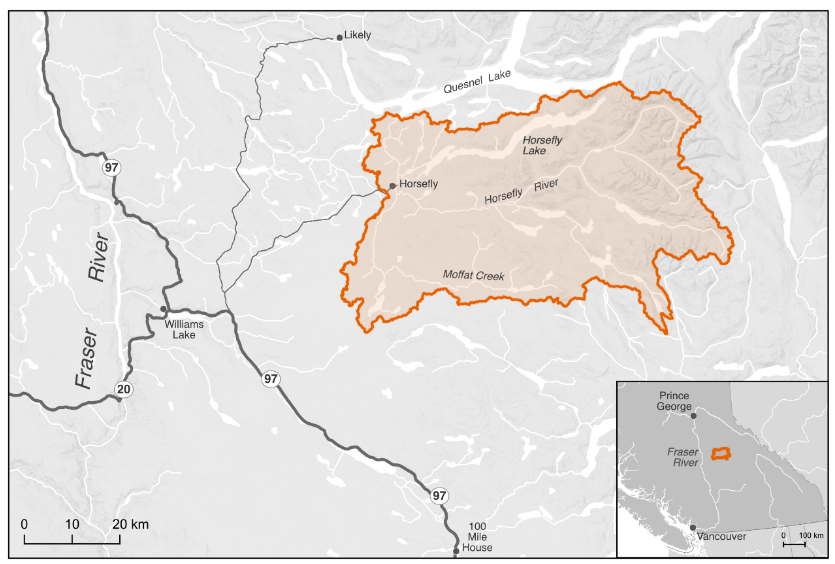
\includegraphics{content/images/geo-scope-hors.png}

}

\caption{\label{fig-geoscope}The primary geographic scope --- the
Quesnel-Bowron watershed, excluding the Morice River (SAMPLE) drainage.}

\end{figure}%

SAMPLE The primary geographic scope of this WCRP is the Bulkley River
watershed, located in the mid-eastern portion of the Skeena River
drainage basin in northwestern British Columbia
(Figure~\ref{fig-geoscope}). The scope constitutes the Bulkley River
``watershed group'' as defined by the
\href{https://catalogue.data.gov.bc.ca/dataset/freshwater-atlas-watershed-groups}{British
Columbia Freshwater Atlas} (FWA). A consistent spatial framework was
necessary to undertake a watershed-selection process at the provincial
scale to identify target watersheds to improve connectivity for
salmonids. The Bulkley River watershed was identified by the BC Fish
Passage Restoration Initiative as one of four target watersheds for WCRP
development Mazany-Wright, Norris, et al. (2021b). The Bulkley River
watershed has a drainage area of 776,200 ha, spanning from Bulkley Lake
in the southeast to the confluence with the Skeena River in the
northwest. The watershed is generally divided into the ``lower'' Bulkley
River and the ``upper'' Bulkley River by the confluence with the Morice
River near the town of Houston. Culturally and economically important
populations of Chinook Salmon (Oncorhynchus tshawytscha), Coho Salmon
(Oncorhynchus kisutch), Sockeye Salmon (Oncorhynchus nerka), and
Steelhead (Oncorhynchus mykiss) are all found in the watershed, which
historically supported Indigenous sustenance and trading economies
(Table~\ref{tbl-spn}; (\textbf{Irvine2021?})).

\begin{longtable}[]{@{}lll@{}}

\caption{\label{tbl-spn}Target fish species in the Bulkley River
watershed. The Gitxsanimax, Witsuwit'en, and Western common and
scientific species names are provided.}

\tabularnewline

\caption{}\label{T_f8f00}\tabularnewline
\toprule\noalign{}
Secwepemctsín & Common Name & Scientific Name \\
\midrule\noalign{}
\endfirsthead
\toprule\noalign{}
Secwepemctsín & Common Name & Scientific Name \\
\midrule\noalign{}
\endhead
\bottomrule\noalign{}
\endlastfoot
Kekèsu & Chinook Salmon & Oncorhynchus tshawytscha \\
Sxeyqs & Coho Salmon & Oncorhynchus kisutch \\
Sqlelten7ùwi & Sockeye Salmon & Oncorhynchus nerka \\

\end{longtable}

SAMPLE The Quesnel-Bowron watershed comprises parts of the traditional
territories of two matrilineal nations:

\begin{itemize}
\item
  SAMPLE Gitxsan peoples-- the traditional Gitxsan Laxyip spans the
  northern portion of the watershed, including the Suskwa River, and is
  governed by a hereditary system of 60 Wilps or House Groups who are
  represented by Simgigyat (hereditary chiefs). Each Wilp has
  jurisdiction over several Anaat, or fishing sites. The Wilp groups
  that have territory coinciding with the Bulkley River watershed
  include Djogaslee, Gyet'm Galdo'o, Luutkudziiwas, Axtii Tsex, Yagosip,
  and Spookw (G. Sebastian pers. comm.). The Gitxsan steward the land
  and waters based on Ayookw (Gitxsan law) and Adaakw (oral histories;
  (\textbf{Gitxsan2019?}), (\textbf{Irvine2021?})). It is necessary to
  receive permission from the individual Wilp chief for any work to
  occur on their territory.
\item
  SAMPLE Wet'suwet'en peoples-- the Wedzin Kwah (Bulkley River
  watershed) is part of the larger Wet'suwet'en traditional territory.
  The hereditary territory is governed by a system made up of five clans
  -- Gilseyhu (Big Frog), Laksilyu (Small Frog), Tsayu (Beaver),
  Gitdumden (Wolf/Bear) and Laksamshu (Fireweed) -- each of which
  comprises multiple Yikhs (House Groups) represented by hereditary
  chiefs. The Wet'suwet'en steward the land based on Inuk Nu'at'en
  (Wet'suwet'en law), and the principle of Yintahk, meaning everything
  is connected to the land ((\textbf{OfficeWetsuweten2013?}),
  (\textbf{Irvine2021?})). It is necessary to receive permission from
  the appropriate bands (Witset First Nation or Wet'suwet'en first
  Nation, Skin Tyee, Nee Tahi Buhn, or Burns Lake Band), nation
  representatives ((\textbf{OfficeWetsuweten2013?})), and the individual
  Yikh chiefs for any work to occur on their territory.
\end{itemize}

The geographic scope of this WCRP was further refined by identifying
``potentially accessible'' stream segments, which are defined as streams
that target species should be able to access in the absence of
anthropogenic barriers (Figure~\ref{fig-strseg}). Potentially accessible
stream segments were spatially delineated using fish species observation
and distribution data, as well as data on ``exclusionary points'', which
are waterfalls greater than 5 m in height and gradient barriers based on
species-specific swimming abilities. These maps were explored by the
planning team to incorporate additional local knowledge, ensure
accuracy, and finalize the constraints on potentially accessible stream
segments. All other stream segments were removed from the scope for
further consideration. The ``constrained geographic scope'' formed the
foundation for all subsequent analyses and planning steps, including
mapping and modelling useable habitat types, quantifying the current
connectivity status, goal setting, and action planning Mazany-Wright,
Norris, et al. (2021a).

\begin{figure}

\centering{

\includegraphics{content/images/accessible-streams-bulk.png}

}

\caption{\label{fig-strseg}SAMPLE Potentially accessible stream segments
within the Bulkley River watershed. These do not represent useable
habitat types, but rather identifies the stream segments within which
habitat modelling and barrier mapping and prioritization was
undertaken.}

\end{figure}%

\section*{Target species}\label{target-species}
\addcontentsline{toc}{section}{Target species}

\markright{Target species}

SAMPLE Target species represent the ecologically and culturally
important species for which habitat connectivity is being conserved
and/or restored in the watershed. In the Bulkley River watershed, the
planning team selected Anadromous Salmonids as the target species group,
which comprises Chinook Salmon, Coho Salmon, Sockeye Salmon, and
Steelhead. Anadromous salmonids also include Pink Salmon (Oncorhynchus
gorbuscha) and Chum Salmon (Oncorhynchus keta) as beneficiary species
(i.e., species that are not actively targeted through the planning
process but will also benefit from connectivity improvements for target
anadromous species in the watershed). The selection of these target
species was driven primarily by the target species of the primary fund
supporting this planning work. The planning team also identified other
culturally and ecologically important species within the watershed to
consider for inclusion in future iterations of the WCRP, including
Pacific Lamprey (Entosphenus tridentatus) and Bull Trout (Salvelinus
confluentus).

\subsection*{SAMPLE Anadromous Salmon}\label{sample-anadromous-salmon}
\addcontentsline{toc}{subsection}{SAMPLE Anadromous Salmon}

Anadromous salmon are cultural and ecological keystone species that
contribute to productive ecosystems by contributing marine-derived
nutrients to the watershed and forming an important food source for
other species. Salmon species are sacred to the NStQ, having sustained
life, trading economies, and culture since time immemorial (W. L. F.
Nation. (2021), X. F. Nation. (2021), N. Singi pers. comm.). The
stewardship of the resources and fisheries in their traditional
territories are imbued in the spirit of the NStQ through a symbiotic
relationship based on respect -- the NStQ never take more salmon than is
needed and there is no waste. The entirety of the salmon is used -
smoked and dried to sustain the NStQ through the winter months, the roe
harvested for consumption, salmon oil rendered to be stored and traded,
and the skin used to store the oil (Wilson, Twohig, and Dahlstrom
(1998), X. F. Nation. (2021), N. Singi pers. comm.). The salmon runs
begin to return to the Horsefly River watershed in early August, and the
NStQ traditionally celebrate and feast at this time. The harvest of the
salmon strengthens the cultural connection to the land and the waters,
providing an important food source for communities and the opportunity
to pass knowledge and ceremony to future generations through fishing and
fish processing (W. L. F. Nation. (2021)`, X. F. Nation. (2021)).

Anadromous salmon populations in the Horsefly River watershed have
declined significantly in the past few decades, with the populations of
all three focal species being listed as Threatened or Endangered by the
Committee On the Status of Endangered Wildlife In Canada (COSEWIC). This
has been exacerbated by the Big Bar landslide on the Fraser River in
2019, leading the four NStQ communities to voluntarily close the salmon
fishery from 2019-2022. The stewardship of their waters continues
through the work of the NStQ member communities and the Northern Shuswap
Tribal Council.

\section*{Barrier Types}\label{barrier-types}
\addcontentsline{toc}{section}{Barrier Types}

\markright{Barrier Types}

SAMPLE The following table highlights which barrier types pose the
greatest threat to in the watershed. The results of this assessment were
used to inform the subsequent planning steps, as well as to identify
knowledge gaps where there is little spatial data to inform the
assessment for a specific barrier type.

\begin{longtable}[]{@{}lllll@{}}

\caption{\label{tbl-barriertype}SAMPLE Connectivity status assessment
for linear habitat (spawning and rearing).}

\tabularnewline

\caption{}\label{T_c0bc4}\tabularnewline
\toprule\noalign{}
Barrier Types & Extent & Severity & Irreversibility & Overall Threat
Rating: \\
\midrule\noalign{}
\endfirsthead
\toprule\noalign{}
Barrier Types & Extent & Severity & Irreversibility & Overall Threat
Rating: \\
\midrule\noalign{}
\endhead
\bottomrule\noalign{}
\endlastfoot
Road-Stream Crossings & Low & Very High & Medium & Very High \\
Lateral Barriers & High & Very High & High & High \\
Small Dams(\textless3m height) & Low & Very High & High & Medium \\
Trail-stream Crossings & Low & Low & Medium & Low \\
Natural Barriers & Medium & High & Low & Low \\

\end{longtable}

\subsection*{Small Dams (\textless3 m
height)}\label{small-dams-3-m-height}
\addcontentsline{toc}{subsection}{Small Dams (\textless3 m height)}

There are \ldots{}

\subsection*{Road-stream Crossings}\label{road-stream-crossings}
\addcontentsline{toc}{subsection}{Road-stream Crossings}

There are \ldots{}

\subsection*{Trail-stream crossings}\label{trail-stream-crossings}
\addcontentsline{toc}{subsection}{Trail-stream crossings}

There are \ldots{}

\subsection*{Lateral Barriers}\label{lateral-barriers}
\addcontentsline{toc}{subsection}{Lateral Barriers}

There are \ldots{}

\subsection*{Natural Barriers}\label{natural-barriers}
\addcontentsline{toc}{subsection}{Natural Barriers}

SAMPLE Natural barriers to fish passage can include debris flows, log
jams, sediment deposits, etc., but natural features that have always
restricted fish passage (e.g., waterfalls) are not considered under this
barrier type. Natural barriers are difficult to include in a spatial
prioritization framework due to their transient nature.

\bookmarksetup{startatroot}

\chapter*{Connectivity Status Assessment and
Goals}\label{connectivity-status-assessment-and-goals}
\addcontentsline{toc}{chapter}{Connectivity Status Assessment and Goals}

\markboth{Connectivity Status Assessment and Goals}{Connectivity Status
Assessment and Goals}

\section*{Key Ecological Attributes and Current Connectivity
Status}\label{key-ecological-attributes-and-current-connectivity-status}
\addcontentsline{toc}{section}{Key Ecological Attributes and Current
Connectivity Status}

\markright{Key Ecological Attributes and Current Connectivity Status}

SAMPLE The planning team devised two Key Ecological Attributes (KEAs)
and associated indicators to assess the current connectivity status of
the watershed -- Accessible Spawning Habitat and Accessible Rearing
Habitat (Table~\ref{tbl-connectivity}). KEAs are the key aspects of
anadromous salmonid ecology that are being targeted by this WCRP. The
connectivity status for the Anadromous Salmonid KEAs were used to
establish goals to improve habitat connectivity in the watershed and
will be the baseline against which progress is tracked over time.

The current connectivity status assessment relies on GIS analyses to map
known and modelled barriers to fish passage, identify stream reaches
that have potential spawning and rearing habitat, estimate the
proportion of habitat that is currently accessible to target species,
and prioritize barriers for field assessment that would provide the
greatest gains in connectivity. To support a flexible prioritization
framework to identify priority barriers in the watershed, two
assumptions are made: 1) any modelled (i.e., passability status is
unknown) or partial barriers are treated as complete barriers to passage
and 2) the habitat modelling is binary, it does not assign any habitat
quality values. As such, the current connectivity status will be refined
over time as more data on habitat and barriers are collected. For more
detail on how the connectivity status assessments were conducted, see
Appendix B.

(see Table~\ref{tbl-connectivity}).

The current connectivity status assessment relies on GIS analyses to map
known and modelled barriers to fish passage, identify stream reaches
that have potential spawning and rearing habitat, estimate the
proportion of habitat that is currently accessible to target species,
and prioritize barriers for field assessment that would provide the
greatest gains in connectivity. To support a flexible prioritization
framework to identify priority barriers in the watershed, two
assumptions are made: 1,any modelled (i.e., passability status is
unknown) or partial barriers are treated as complete barriers to passage
and 2, the habitat modelling is binary, it does not assign any habitat
quality values. As such, the current connectivity status will be refined
over time as more data on habitat and barriers are collected. For more
detail on how the connectivity status assessments were conducted, see
Data Download and Methods.

\begin{longtable}[]{@{}lllllll@{}}

\caption{\label{tbl-connectivity}SAMPLE TABLE Connectivity status
assessment for spawning and rearing habitat.}

\tabularnewline

\caption{}\label{T_01924}\tabularnewline
\toprule\noalign{}
Target Species & KEA & Indicator & Poor & Fair & Good & Very Good \\
\midrule\noalign{}
\endfirsthead
\toprule\noalign{}
Target Species & KEA & Indicator & Poor & Fair & Good & Very Good \\
\midrule\noalign{}
\endhead
\bottomrule\noalign{}
\endlastfoot
Andromous Salmon & Available Spawning Habitat & \% of total habitat &
\textless50\% & 51-75\% & 76-90\% & \textgreater90\% \\
& & Current Status: & & & 85 & \\

\end{longtable}

\section*{Goals}\label{goals}
\addcontentsline{toc}{section}{Goals}

\markright{Goals}

\begin{longtable}[]{@{}ll@{}}

\caption{\label{tbl-goals}SAMPLE TABLE Goals to improve spawning and
rearing habitat connectivity for target species in the watershed. The
goals were established through discussions with the planning team and
represent the resulting desired state of connectivity in the watershed.
The goals are subject to change as more information and data are
collected over the course of the plan timeline (e.g., the current
connectivity status is updated based on barrier field assessments).}

\tabularnewline

\caption{}\label{T_4505c}\tabularnewline
\toprule\noalign{}
Goal \# & Goal \\
\midrule\noalign{}
\endfirsthead
\toprule\noalign{}
Goal \# & Goal \\
\midrule\noalign{}
\endhead
\bottomrule\noalign{}
\endlastfoot
1 & By 2040, the percent (\%) of total linear habitat accessible to
anadromous salmon will increase from 85\% to 96\% within the Horsefly
River watershed (i.e., reconnect at least 261.97 km of habitat). \\
2 & By 2024, the total area of overwintering habitat accessible to
Anadromous Salmon will increase by 1,500 m2 within the Horsefly River
watershed. \\

\end{longtable}

\bookmarksetup{startatroot}

\chapter*{Barrier Prioritization}\label{barrier-prioritization}
\addcontentsline{toc}{chapter}{Barrier Prioritization}

\markboth{Barrier Prioritization}{Barrier Prioritization}

\section*{Quesnel-Bowron Watershed Barrier Prioritization
Summary}\label{quesnel-bowron-watershed-barrier-prioritization-summary}
\addcontentsline{toc}{section}{Quesnel-Bowron Watershed Barrier
Prioritization Summary}

\markright{Quesnel-Bowron Watershed Barrier Prioritization Summary}

SAMPLE The primary conservation outcome of the WCRP is the remediation
of barriers to connectivity in the Quesnel-Bowron watershed. To achieve
Goals 1 and 2 in this plan, it is necessary to prioritize and identify a
suite of barriers that, if remediated, will provide access to a minimum
of 86 km of spawning habitat and 211 km of rearing habitat
(\textbf{?@tbl-table16}):

\begin{longtable}[]{@{}llllll@{}}

\caption{\label{tbl-gainReqs}SAMPLE Spawning and rearing habitat
connectivity gain requirements to meet WCRP goals in Quesnel-Bowron
watershed. The measures of currently accessible and total habitat values
are derived from the Intrinsic Potential habitat model.}

\tabularnewline

\caption{}\label{T_048ae}\tabularnewline
\toprule\noalign{}
Habitat Type & Currently accessible (km) & Total & Current Connectivity
Status & Goal & Gain required (km) \\
\midrule\noalign{}
\endfirsthead
\toprule\noalign{}
Habitat Type & Currently accessible (km) & Total & Current Connectivity
Status & Goal & Gain required (km) \\
\midrule\noalign{}
\endhead
\bottomrule\noalign{}
\endlastfoot
Spawning and Rearing & 4045.69 & 4487.15 & 85\% & 96\% & 261.97 \\

\end{longtable}

The barrier prioritization process comprises three stages:

\begin{itemize}
\item
  Stage 1: preliminary barrier list
\item
  Stage 2: intermediate barrier list
\item
  Stage 3: priority barrier list
\end{itemize}

SAMPLE The barrier prioritization analysis ranked barriers by
{[}\ldots{]} A longer list of barriers is needed due to the inherent
assumptions in the connectivity model, habitat model, and gaps in
available data. Barriers that have been modelled (i.e., points where
streams and road/rail networks intersect) are assumed to be barriers
until field verification is undertaken and structures that have been
assessed as ``potential'' barriers (e.g., may be passable at certain
flow levels or for certain life history stages) require further
investigation before a definitive remediation decision is made.
Additionally, the habitat model identifies stream segments that have the
potential to support spawning or rearing habitat for target species but
does not attempt to quantify habitat quality or suitability (see
Appendix B), which will require additional field verification once
barrier assessments have completed.Data deficient structures represents
structures that are a priority to evaluate further through barrier
assessment and habitat confirmations because some structures will likely
be passable, others will not be associated with usable habitat, and
others may not be feasible to remediate because of logistic
considerations (Table~\ref{tbl-deficient}). Some barriers were moved
forward to the ``priority barrier list'' (see Table~\ref{tbl-priority})
and others were eliminated from consideration due to one or more of the
considerations discussed above (see Table~\ref{tbl-remove}). The
priority barrier list represents structures that were confirmed to be
partial or full barriers to fish passage and that block access to
confirmed habitat. Barriers on the priority list were reviewed by
planning team members and selected for inclusion for proactive pursual
of remediation. For more details on the barrier prioritization model,
please see Mazany-Wright, Norris, et al. (2021a).

\global\setlength{\Oldarrayrulewidth}{\arrayrulewidth}

\global\setlength{\Oldtabcolsep}{\tabcolsep}

\setlength{\tabcolsep}{2pt}

\renewcommand*{\arraystretch}{1.5}



\providecommand{\ascline}[3]{\noalign{\global\arrayrulewidth #1}\arrayrulecolor[HTML]{#2}\cline{#3}}

\begin{longtable}[c]{|p{0.44in}|p{1.58in}|p{1.08in}|p{1.70in}|p{1.07in}|p{1.20in}|p{1.61in}|p{1.34in}|p{2.43in}|p{1.93in}|p{1.81in}|p{2.23in}|p{2.06in}|p{1.01in}|p{0.81in}}

\caption{\label{tbl-priority}SAMPLE priority barrier list, which
includes barriers that have undergone field assessment, been reviewed by
the planning team, and selected to pursue for proactive remediation.}

\tabularnewline

\hhline{>{\arrayrulecolor[HTML]{666666}\global\arrayrulewidth=1.5pt}->{\arrayrulecolor[HTML]{666666}\global\arrayrulewidth=1.5pt}->{\arrayrulecolor[HTML]{666666}\global\arrayrulewidth=1.5pt}->{\arrayrulecolor[HTML]{666666}\global\arrayrulewidth=1.5pt}->{\arrayrulecolor[HTML]{666666}\global\arrayrulewidth=1.5pt}->{\arrayrulecolor[HTML]{666666}\global\arrayrulewidth=1.5pt}->{\arrayrulecolor[HTML]{666666}\global\arrayrulewidth=1.5pt}->{\arrayrulecolor[HTML]{666666}\global\arrayrulewidth=1.5pt}->{\arrayrulecolor[HTML]{666666}\global\arrayrulewidth=1.5pt}->{\arrayrulecolor[HTML]{666666}\global\arrayrulewidth=1.5pt}->{\arrayrulecolor[HTML]{666666}\global\arrayrulewidth=1.5pt}->{\arrayrulecolor[HTML]{666666}\global\arrayrulewidth=1.5pt}->{\arrayrulecolor[HTML]{666666}\global\arrayrulewidth=1.5pt}->{\arrayrulecolor[HTML]{666666}\global\arrayrulewidth=1.5pt}->{\arrayrulecolor[HTML]{666666}\global\arrayrulewidth=1.5pt}-}

\multicolumn{1}{>{\cellcolor[HTML]{008270}\raggedright}m{\dimexpr 0.44in+0\tabcolsep}}{\textcolor[HTML]{FFFFFF}{\fontsize{11}{11}\selectfont{\global\setmainfont{Arial}{ID}}}} & \multicolumn{1}{>{\cellcolor[HTML]{008270}\raggedright}m{\dimexpr 1.58in+0\tabcolsep}}{\textcolor[HTML]{FFFFFF}{\fontsize{11}{11}\selectfont{\global\setmainfont{Arial}{Watercourse\ name}}}} & \multicolumn{1}{>{\cellcolor[HTML]{008270}\raggedright}m{\dimexpr 1.08in+0\tabcolsep}}{\textcolor[HTML]{FFFFFF}{\fontsize{11}{11}\selectfont{\global\setmainfont{Arial}{Road\ name}}}} & \multicolumn{1}{>{\cellcolor[HTML]{008270}\raggedright}m{\dimexpr 1.7in+0\tabcolsep}}{\textcolor[HTML]{FFFFFF}{\fontsize{11}{11}\selectfont{\global\setmainfont{Arial}{Location/coordinates}}}} & \multicolumn{1}{>{\cellcolor[HTML]{008270}\raggedright}m{\dimexpr 1.07in+0\tabcolsep}}{\textcolor[HTML]{FFFFFF}{\fontsize{11}{11}\selectfont{\global\setmainfont{Arial}{Barrier\ type}}}} & \multicolumn{1}{>{\cellcolor[HTML]{008270}\raggedright}m{\dimexpr 1.2in+0\tabcolsep}}{\textcolor[HTML]{FFFFFF}{\fontsize{11}{11}\selectfont{\global\setmainfont{Arial}{Barrier\ owner}}}} & \multicolumn{1}{>{\cellcolor[HTML]{008270}\raggedright}m{\dimexpr 1.61in+0\tabcolsep}}{\textcolor[HTML]{FFFFFF}{\fontsize{11}{11}\selectfont{\global\setmainfont{Arial}{Barrier\ set\ identifier}}}} & \multicolumn{1}{>{\cellcolor[HTML]{008270}\raggedright}m{\dimexpr 1.34in+0\tabcolsep}}{\textcolor[HTML]{FFFFFF}{\fontsize{11}{11}\selectfont{\global\setmainfont{Arial}{\#\ barriers\ in\ set}}}} & \multicolumn{1}{>{\cellcolor[HTML]{008270}\raggedright}m{\dimexpr 2.43in+0\tabcolsep}}{\textcolor[HTML]{FFFFFF}{\fontsize{11}{11}\selectfont{\global\setmainfont{Arial}{Number\ of\ downstream\ barriers}}}} & \multicolumn{1}{>{\cellcolor[HTML]{008270}\raggedright}m{\dimexpr 1.93in+0\tabcolsep}}{\textcolor[HTML]{FFFFFF}{\fontsize{11}{11}\selectfont{\global\setmainfont{Arial}{Upstream\ habitat\ quality}}}} & \multicolumn{1}{>{\cellcolor[HTML]{008270}\raggedright}m{\dimexpr 1.81in+0\tabcolsep}}{\textcolor[HTML]{FFFFFF}{\fontsize{11}{11}\selectfont{\global\setmainfont{Arial}{Total\ habitat\ gain\ (km)}}}} & \multicolumn{1}{>{\cellcolor[HTML]{008270}\raggedright}m{\dimexpr 2.23in+0\tabcolsep}}{\textcolor[HTML]{FFFFFF}{\fontsize{11}{11}\selectfont{\global\setmainfont{Arial}{Habitat\ gain\ -\ spawning\ (km)}}}} & \multicolumn{1}{>{\cellcolor[HTML]{008270}\raggedright}m{\dimexpr 2.06in+0\tabcolsep}}{\textcolor[HTML]{FFFFFF}{\fontsize{11}{11}\selectfont{\global\setmainfont{Arial}{Habitat\ gain\ -\ rearing\ (km)}}}} & \multicolumn{1}{>{\cellcolor[HTML]{008270}\raggedright}m{\dimexpr 1.01in+0\tabcolsep}}{\textcolor[HTML]{FFFFFF}{\fontsize{11}{11}\selectfont{\global\setmainfont{Arial}{Next\ steps}}}} & \multicolumn{1}{>{\cellcolor[HTML]{008270}\raggedright}m{\dimexpr 0.81in+0\tabcolsep}}{\textcolor[HTML]{FFFFFF}{\fontsize{11}{11}\selectfont{\global\setmainfont{Arial}{Reason}}}} \\

\noalign{\global\arrayrulewidth 0pt}\arrayrulecolor[HTML]{000000}

\hhline{>{\arrayrulecolor[HTML]{666666}\global\arrayrulewidth=1.5pt}->{\arrayrulecolor[HTML]{666666}\global\arrayrulewidth=1.5pt}->{\arrayrulecolor[HTML]{666666}\global\arrayrulewidth=1.5pt}->{\arrayrulecolor[HTML]{666666}\global\arrayrulewidth=1.5pt}->{\arrayrulecolor[HTML]{666666}\global\arrayrulewidth=1.5pt}->{\arrayrulecolor[HTML]{666666}\global\arrayrulewidth=1.5pt}->{\arrayrulecolor[HTML]{666666}\global\arrayrulewidth=1.5pt}->{\arrayrulecolor[HTML]{666666}\global\arrayrulewidth=1.5pt}->{\arrayrulecolor[HTML]{666666}\global\arrayrulewidth=1.5pt}->{\arrayrulecolor[HTML]{666666}\global\arrayrulewidth=1.5pt}->{\arrayrulecolor[HTML]{666666}\global\arrayrulewidth=1.5pt}->{\arrayrulecolor[HTML]{666666}\global\arrayrulewidth=1.5pt}->{\arrayrulecolor[HTML]{666666}\global\arrayrulewidth=1.5pt}->{\arrayrulecolor[HTML]{666666}\global\arrayrulewidth=1.5pt}->{\arrayrulecolor[HTML]{666666}\global\arrayrulewidth=1.5pt}-}\endfirsthead 

\hhline{>{\arrayrulecolor[HTML]{666666}\global\arrayrulewidth=1.5pt}->{\arrayrulecolor[HTML]{666666}\global\arrayrulewidth=1.5pt}->{\arrayrulecolor[HTML]{666666}\global\arrayrulewidth=1.5pt}->{\arrayrulecolor[HTML]{666666}\global\arrayrulewidth=1.5pt}->{\arrayrulecolor[HTML]{666666}\global\arrayrulewidth=1.5pt}->{\arrayrulecolor[HTML]{666666}\global\arrayrulewidth=1.5pt}->{\arrayrulecolor[HTML]{666666}\global\arrayrulewidth=1.5pt}->{\arrayrulecolor[HTML]{666666}\global\arrayrulewidth=1.5pt}->{\arrayrulecolor[HTML]{666666}\global\arrayrulewidth=1.5pt}->{\arrayrulecolor[HTML]{666666}\global\arrayrulewidth=1.5pt}->{\arrayrulecolor[HTML]{666666}\global\arrayrulewidth=1.5pt}->{\arrayrulecolor[HTML]{666666}\global\arrayrulewidth=1.5pt}->{\arrayrulecolor[HTML]{666666}\global\arrayrulewidth=1.5pt}->{\arrayrulecolor[HTML]{666666}\global\arrayrulewidth=1.5pt}->{\arrayrulecolor[HTML]{666666}\global\arrayrulewidth=1.5pt}-}

\multicolumn{1}{>{\cellcolor[HTML]{008270}\raggedright}m{\dimexpr 0.44in+0\tabcolsep}}{\textcolor[HTML]{FFFFFF}{\fontsize{11}{11}\selectfont{\global\setmainfont{Arial}{ID}}}} & \multicolumn{1}{>{\cellcolor[HTML]{008270}\raggedright}m{\dimexpr 1.58in+0\tabcolsep}}{\textcolor[HTML]{FFFFFF}{\fontsize{11}{11}\selectfont{\global\setmainfont{Arial}{Watercourse\ name}}}} & \multicolumn{1}{>{\cellcolor[HTML]{008270}\raggedright}m{\dimexpr 1.08in+0\tabcolsep}}{\textcolor[HTML]{FFFFFF}{\fontsize{11}{11}\selectfont{\global\setmainfont{Arial}{Road\ name}}}} & \multicolumn{1}{>{\cellcolor[HTML]{008270}\raggedright}m{\dimexpr 1.7in+0\tabcolsep}}{\textcolor[HTML]{FFFFFF}{\fontsize{11}{11}\selectfont{\global\setmainfont{Arial}{Location/coordinates}}}} & \multicolumn{1}{>{\cellcolor[HTML]{008270}\raggedright}m{\dimexpr 1.07in+0\tabcolsep}}{\textcolor[HTML]{FFFFFF}{\fontsize{11}{11}\selectfont{\global\setmainfont{Arial}{Barrier\ type}}}} & \multicolumn{1}{>{\cellcolor[HTML]{008270}\raggedright}m{\dimexpr 1.2in+0\tabcolsep}}{\textcolor[HTML]{FFFFFF}{\fontsize{11}{11}\selectfont{\global\setmainfont{Arial}{Barrier\ owner}}}} & \multicolumn{1}{>{\cellcolor[HTML]{008270}\raggedright}m{\dimexpr 1.61in+0\tabcolsep}}{\textcolor[HTML]{FFFFFF}{\fontsize{11}{11}\selectfont{\global\setmainfont{Arial}{Barrier\ set\ identifier}}}} & \multicolumn{1}{>{\cellcolor[HTML]{008270}\raggedright}m{\dimexpr 1.34in+0\tabcolsep}}{\textcolor[HTML]{FFFFFF}{\fontsize{11}{11}\selectfont{\global\setmainfont{Arial}{\#\ barriers\ in\ set}}}} & \multicolumn{1}{>{\cellcolor[HTML]{008270}\raggedright}m{\dimexpr 2.43in+0\tabcolsep}}{\textcolor[HTML]{FFFFFF}{\fontsize{11}{11}\selectfont{\global\setmainfont{Arial}{Number\ of\ downstream\ barriers}}}} & \multicolumn{1}{>{\cellcolor[HTML]{008270}\raggedright}m{\dimexpr 1.93in+0\tabcolsep}}{\textcolor[HTML]{FFFFFF}{\fontsize{11}{11}\selectfont{\global\setmainfont{Arial}{Upstream\ habitat\ quality}}}} & \multicolumn{1}{>{\cellcolor[HTML]{008270}\raggedright}m{\dimexpr 1.81in+0\tabcolsep}}{\textcolor[HTML]{FFFFFF}{\fontsize{11}{11}\selectfont{\global\setmainfont{Arial}{Total\ habitat\ gain\ (km)}}}} & \multicolumn{1}{>{\cellcolor[HTML]{008270}\raggedright}m{\dimexpr 2.23in+0\tabcolsep}}{\textcolor[HTML]{FFFFFF}{\fontsize{11}{11}\selectfont{\global\setmainfont{Arial}{Habitat\ gain\ -\ spawning\ (km)}}}} & \multicolumn{1}{>{\cellcolor[HTML]{008270}\raggedright}m{\dimexpr 2.06in+0\tabcolsep}}{\textcolor[HTML]{FFFFFF}{\fontsize{11}{11}\selectfont{\global\setmainfont{Arial}{Habitat\ gain\ -\ rearing\ (km)}}}} & \multicolumn{1}{>{\cellcolor[HTML]{008270}\raggedright}m{\dimexpr 1.01in+0\tabcolsep}}{\textcolor[HTML]{FFFFFF}{\fontsize{11}{11}\selectfont{\global\setmainfont{Arial}{Next\ steps}}}} & \multicolumn{1}{>{\cellcolor[HTML]{008270}\raggedright}m{\dimexpr 0.81in+0\tabcolsep}}{\textcolor[HTML]{FFFFFF}{\fontsize{11}{11}\selectfont{\global\setmainfont{Arial}{Reason}}}} \\

\noalign{\global\arrayrulewidth 0pt}\arrayrulecolor[HTML]{000000}

\hhline{>{\arrayrulecolor[HTML]{666666}\global\arrayrulewidth=1.5pt}->{\arrayrulecolor[HTML]{666666}\global\arrayrulewidth=1.5pt}->{\arrayrulecolor[HTML]{666666}\global\arrayrulewidth=1.5pt}->{\arrayrulecolor[HTML]{666666}\global\arrayrulewidth=1.5pt}->{\arrayrulecolor[HTML]{666666}\global\arrayrulewidth=1.5pt}->{\arrayrulecolor[HTML]{666666}\global\arrayrulewidth=1.5pt}->{\arrayrulecolor[HTML]{666666}\global\arrayrulewidth=1.5pt}->{\arrayrulecolor[HTML]{666666}\global\arrayrulewidth=1.5pt}->{\arrayrulecolor[HTML]{666666}\global\arrayrulewidth=1.5pt}->{\arrayrulecolor[HTML]{666666}\global\arrayrulewidth=1.5pt}->{\arrayrulecolor[HTML]{666666}\global\arrayrulewidth=1.5pt}->{\arrayrulecolor[HTML]{666666}\global\arrayrulewidth=1.5pt}->{\arrayrulecolor[HTML]{666666}\global\arrayrulewidth=1.5pt}->{\arrayrulecolor[HTML]{666666}\global\arrayrulewidth=1.5pt}->{\arrayrulecolor[HTML]{666666}\global\arrayrulewidth=1.5pt}-}\endhead


\end{longtable}

\arrayrulecolor[HTML]{000000}

\global\setlength{\arrayrulewidth}{\Oldarrayrulewidth}

\global\setlength{\tabcolsep}{\Oldtabcolsep}

\renewcommand*{\arraystretch}{1}

\global\setlength{\Oldarrayrulewidth}{\arrayrulewidth}

\global\setlength{\Oldtabcolsep}{\tabcolsep}

\setlength{\tabcolsep}{2pt}

\renewcommand*{\arraystretch}{1.5}



\providecommand{\ascline}[3]{\noalign{\global\arrayrulewidth #1}\arrayrulecolor[HTML]{#2}\cline{#3}}

\begin{longtable}[c]{|p{0.44in}|p{1.58in}|p{1.08in}|p{1.70in}|p{2.20in}|p{1.49in}|p{1.81in}|p{2.23in}|p{2.06in}|p{1.24in}|p{1.61in}|p{1.43in}|p{2.43in}|p{1.01in}|p{1.71in}}

\caption{\label{tbl-deficient}Assessed structures that remain data
deficient}

\tabularnewline

\hhline{>{\arrayrulecolor[HTML]{666666}\global\arrayrulewidth=1.5pt}->{\arrayrulecolor[HTML]{666666}\global\arrayrulewidth=1.5pt}->{\arrayrulecolor[HTML]{666666}\global\arrayrulewidth=1.5pt}->{\arrayrulecolor[HTML]{666666}\global\arrayrulewidth=1.5pt}->{\arrayrulecolor[HTML]{666666}\global\arrayrulewidth=1.5pt}->{\arrayrulecolor[HTML]{666666}\global\arrayrulewidth=1.5pt}->{\arrayrulecolor[HTML]{666666}\global\arrayrulewidth=1.5pt}->{\arrayrulecolor[HTML]{666666}\global\arrayrulewidth=1.5pt}->{\arrayrulecolor[HTML]{666666}\global\arrayrulewidth=1.5pt}->{\arrayrulecolor[HTML]{666666}\global\arrayrulewidth=1.5pt}->{\arrayrulecolor[HTML]{666666}\global\arrayrulewidth=1.5pt}->{\arrayrulecolor[HTML]{666666}\global\arrayrulewidth=1.5pt}->{\arrayrulecolor[HTML]{666666}\global\arrayrulewidth=1.5pt}->{\arrayrulecolor[HTML]{666666}\global\arrayrulewidth=1.5pt}->{\arrayrulecolor[HTML]{666666}\global\arrayrulewidth=1.5pt}-}

\multicolumn{1}{>{\cellcolor[HTML]{008270}\raggedright}m{\dimexpr 0.44in+0\tabcolsep}}{\textcolor[HTML]{FFFFFF}{\fontsize{11}{11}\selectfont{\global\setmainfont{Arial}{ID}}}} & \multicolumn{1}{>{\cellcolor[HTML]{008270}\raggedright}m{\dimexpr 1.58in+0\tabcolsep}}{\textcolor[HTML]{FFFFFF}{\fontsize{11}{11}\selectfont{\global\setmainfont{Arial}{Watercourse\ name}}}} & \multicolumn{1}{>{\cellcolor[HTML]{008270}\raggedright}m{\dimexpr 1.08in+0\tabcolsep}}{\textcolor[HTML]{FFFFFF}{\fontsize{11}{11}\selectfont{\global\setmainfont{Arial}{Road\ name}}}} & \multicolumn{1}{>{\cellcolor[HTML]{008270}\raggedright}m{\dimexpr 1.7in+0\tabcolsep}}{\textcolor[HTML]{FFFFFF}{\fontsize{11}{11}\selectfont{\global\setmainfont{Arial}{Location/coordinates}}}} & \multicolumn{1}{>{\cellcolor[HTML]{008270}\raggedright}m{\dimexpr 2.2in+0\tabcolsep}}{\textcolor[HTML]{FFFFFF}{\fontsize{11}{11}\selectfont{\global\setmainfont{Arial}{Assessment\ step\ completed}}}} & \multicolumn{1}{>{\cellcolor[HTML]{008270}\raggedright}m{\dimexpr 1.49in+0\tabcolsep}}{\textcolor[HTML]{FFFFFF}{\fontsize{11}{11}\selectfont{\global\setmainfont{Arial}{Passability\ Status}}}} & \multicolumn{1}{>{\cellcolor[HTML]{008270}\raggedright}m{\dimexpr 1.81in+0\tabcolsep}}{\textcolor[HTML]{FFFFFF}{\fontsize{11}{11}\selectfont{\global\setmainfont{Arial}{Total\ habitat\ gain\ (km)}}}} & \multicolumn{1}{>{\cellcolor[HTML]{008270}\raggedright}m{\dimexpr 2.23in+0\tabcolsep}}{\textcolor[HTML]{FFFFFF}{\fontsize{11}{11}\selectfont{\global\setmainfont{Arial}{Habitat\ gain\ -\ spawning\ (km)}}}} & \multicolumn{1}{>{\cellcolor[HTML]{008270}\raggedright}m{\dimexpr 2.06in+0\tabcolsep}}{\textcolor[HTML]{FFFFFF}{\fontsize{11}{11}\selectfont{\global\setmainfont{Arial}{Habitat\ gain\ -\ rearing\ (km)}}}} & \multicolumn{1}{>{\cellcolor[HTML]{008270}\raggedright}m{\dimexpr 1.24in+0\tabcolsep}}{\textcolor[HTML]{FFFFFF}{\fontsize{11}{11}\selectfont{\global\setmainfont{Arial}{Structure\ type}}}} & \multicolumn{1}{>{\cellcolor[HTML]{008270}\raggedright}m{\dimexpr 1.61in+0\tabcolsep}}{\textcolor[HTML]{FFFFFF}{\fontsize{11}{11}\selectfont{\global\setmainfont{Arial}{Barrier\ set\ identifier}}}} & \multicolumn{1}{>{\cellcolor[HTML]{008270}\raggedright}m{\dimexpr 1.43in+0\tabcolsep}}{\textcolor[HTML]{FFFFFF}{\fontsize{11}{11}\selectfont{\global\setmainfont{Arial}{\#\ of\ barrier\ in\ set}}}} & \multicolumn{1}{>{\cellcolor[HTML]{008270}\raggedright}m{\dimexpr 2.43in+0\tabcolsep}}{\textcolor[HTML]{FFFFFF}{\fontsize{11}{11}\selectfont{\global\setmainfont{Arial}{Number\ of\ downstream\ barriers}}}} & \multicolumn{1}{>{\cellcolor[HTML]{008270}\raggedright}m{\dimexpr 1.01in+0\tabcolsep}}{\textcolor[HTML]{FFFFFF}{\fontsize{11}{11}\selectfont{\global\setmainfont{Arial}{Next\ steps}}}} & \multicolumn{1}{>{\cellcolor[HTML]{008270}\raggedright}m{\dimexpr 1.71in+0\tabcolsep}}{\textcolor[HTML]{FFFFFF}{\fontsize{11}{11}\selectfont{\global\setmainfont{Arial}{Comments\ (external)}}}} \\

\noalign{\global\arrayrulewidth 0pt}\arrayrulecolor[HTML]{000000}

\hhline{>{\arrayrulecolor[HTML]{666666}\global\arrayrulewidth=1.5pt}->{\arrayrulecolor[HTML]{666666}\global\arrayrulewidth=1.5pt}->{\arrayrulecolor[HTML]{666666}\global\arrayrulewidth=1.5pt}->{\arrayrulecolor[HTML]{666666}\global\arrayrulewidth=1.5pt}->{\arrayrulecolor[HTML]{666666}\global\arrayrulewidth=1.5pt}->{\arrayrulecolor[HTML]{666666}\global\arrayrulewidth=1.5pt}->{\arrayrulecolor[HTML]{666666}\global\arrayrulewidth=1.5pt}->{\arrayrulecolor[HTML]{666666}\global\arrayrulewidth=1.5pt}->{\arrayrulecolor[HTML]{666666}\global\arrayrulewidth=1.5pt}->{\arrayrulecolor[HTML]{666666}\global\arrayrulewidth=1.5pt}->{\arrayrulecolor[HTML]{666666}\global\arrayrulewidth=1.5pt}->{\arrayrulecolor[HTML]{666666}\global\arrayrulewidth=1.5pt}->{\arrayrulecolor[HTML]{666666}\global\arrayrulewidth=1.5pt}->{\arrayrulecolor[HTML]{666666}\global\arrayrulewidth=1.5pt}->{\arrayrulecolor[HTML]{666666}\global\arrayrulewidth=1.5pt}-}\endfirsthead 

\hhline{>{\arrayrulecolor[HTML]{666666}\global\arrayrulewidth=1.5pt}->{\arrayrulecolor[HTML]{666666}\global\arrayrulewidth=1.5pt}->{\arrayrulecolor[HTML]{666666}\global\arrayrulewidth=1.5pt}->{\arrayrulecolor[HTML]{666666}\global\arrayrulewidth=1.5pt}->{\arrayrulecolor[HTML]{666666}\global\arrayrulewidth=1.5pt}->{\arrayrulecolor[HTML]{666666}\global\arrayrulewidth=1.5pt}->{\arrayrulecolor[HTML]{666666}\global\arrayrulewidth=1.5pt}->{\arrayrulecolor[HTML]{666666}\global\arrayrulewidth=1.5pt}->{\arrayrulecolor[HTML]{666666}\global\arrayrulewidth=1.5pt}->{\arrayrulecolor[HTML]{666666}\global\arrayrulewidth=1.5pt}->{\arrayrulecolor[HTML]{666666}\global\arrayrulewidth=1.5pt}->{\arrayrulecolor[HTML]{666666}\global\arrayrulewidth=1.5pt}->{\arrayrulecolor[HTML]{666666}\global\arrayrulewidth=1.5pt}->{\arrayrulecolor[HTML]{666666}\global\arrayrulewidth=1.5pt}->{\arrayrulecolor[HTML]{666666}\global\arrayrulewidth=1.5pt}-}

\multicolumn{1}{>{\cellcolor[HTML]{008270}\raggedright}m{\dimexpr 0.44in+0\tabcolsep}}{\textcolor[HTML]{FFFFFF}{\fontsize{11}{11}\selectfont{\global\setmainfont{Arial}{ID}}}} & \multicolumn{1}{>{\cellcolor[HTML]{008270}\raggedright}m{\dimexpr 1.58in+0\tabcolsep}}{\textcolor[HTML]{FFFFFF}{\fontsize{11}{11}\selectfont{\global\setmainfont{Arial}{Watercourse\ name}}}} & \multicolumn{1}{>{\cellcolor[HTML]{008270}\raggedright}m{\dimexpr 1.08in+0\tabcolsep}}{\textcolor[HTML]{FFFFFF}{\fontsize{11}{11}\selectfont{\global\setmainfont{Arial}{Road\ name}}}} & \multicolumn{1}{>{\cellcolor[HTML]{008270}\raggedright}m{\dimexpr 1.7in+0\tabcolsep}}{\textcolor[HTML]{FFFFFF}{\fontsize{11}{11}\selectfont{\global\setmainfont{Arial}{Location/coordinates}}}} & \multicolumn{1}{>{\cellcolor[HTML]{008270}\raggedright}m{\dimexpr 2.2in+0\tabcolsep}}{\textcolor[HTML]{FFFFFF}{\fontsize{11}{11}\selectfont{\global\setmainfont{Arial}{Assessment\ step\ completed}}}} & \multicolumn{1}{>{\cellcolor[HTML]{008270}\raggedright}m{\dimexpr 1.49in+0\tabcolsep}}{\textcolor[HTML]{FFFFFF}{\fontsize{11}{11}\selectfont{\global\setmainfont{Arial}{Passability\ Status}}}} & \multicolumn{1}{>{\cellcolor[HTML]{008270}\raggedright}m{\dimexpr 1.81in+0\tabcolsep}}{\textcolor[HTML]{FFFFFF}{\fontsize{11}{11}\selectfont{\global\setmainfont{Arial}{Total\ habitat\ gain\ (km)}}}} & \multicolumn{1}{>{\cellcolor[HTML]{008270}\raggedright}m{\dimexpr 2.23in+0\tabcolsep}}{\textcolor[HTML]{FFFFFF}{\fontsize{11}{11}\selectfont{\global\setmainfont{Arial}{Habitat\ gain\ -\ spawning\ (km)}}}} & \multicolumn{1}{>{\cellcolor[HTML]{008270}\raggedright}m{\dimexpr 2.06in+0\tabcolsep}}{\textcolor[HTML]{FFFFFF}{\fontsize{11}{11}\selectfont{\global\setmainfont{Arial}{Habitat\ gain\ -\ rearing\ (km)}}}} & \multicolumn{1}{>{\cellcolor[HTML]{008270}\raggedright}m{\dimexpr 1.24in+0\tabcolsep}}{\textcolor[HTML]{FFFFFF}{\fontsize{11}{11}\selectfont{\global\setmainfont{Arial}{Structure\ type}}}} & \multicolumn{1}{>{\cellcolor[HTML]{008270}\raggedright}m{\dimexpr 1.61in+0\tabcolsep}}{\textcolor[HTML]{FFFFFF}{\fontsize{11}{11}\selectfont{\global\setmainfont{Arial}{Barrier\ set\ identifier}}}} & \multicolumn{1}{>{\cellcolor[HTML]{008270}\raggedright}m{\dimexpr 1.43in+0\tabcolsep}}{\textcolor[HTML]{FFFFFF}{\fontsize{11}{11}\selectfont{\global\setmainfont{Arial}{\#\ of\ barrier\ in\ set}}}} & \multicolumn{1}{>{\cellcolor[HTML]{008270}\raggedright}m{\dimexpr 2.43in+0\tabcolsep}}{\textcolor[HTML]{FFFFFF}{\fontsize{11}{11}\selectfont{\global\setmainfont{Arial}{Number\ of\ downstream\ barriers}}}} & \multicolumn{1}{>{\cellcolor[HTML]{008270}\raggedright}m{\dimexpr 1.01in+0\tabcolsep}}{\textcolor[HTML]{FFFFFF}{\fontsize{11}{11}\selectfont{\global\setmainfont{Arial}{Next\ steps}}}} & \multicolumn{1}{>{\cellcolor[HTML]{008270}\raggedright}m{\dimexpr 1.71in+0\tabcolsep}}{\textcolor[HTML]{FFFFFF}{\fontsize{11}{11}\selectfont{\global\setmainfont{Arial}{Comments\ (external)}}}} \\

\noalign{\global\arrayrulewidth 0pt}\arrayrulecolor[HTML]{000000}

\hhline{>{\arrayrulecolor[HTML]{666666}\global\arrayrulewidth=1.5pt}->{\arrayrulecolor[HTML]{666666}\global\arrayrulewidth=1.5pt}->{\arrayrulecolor[HTML]{666666}\global\arrayrulewidth=1.5pt}->{\arrayrulecolor[HTML]{666666}\global\arrayrulewidth=1.5pt}->{\arrayrulecolor[HTML]{666666}\global\arrayrulewidth=1.5pt}->{\arrayrulecolor[HTML]{666666}\global\arrayrulewidth=1.5pt}->{\arrayrulecolor[HTML]{666666}\global\arrayrulewidth=1.5pt}->{\arrayrulecolor[HTML]{666666}\global\arrayrulewidth=1.5pt}->{\arrayrulecolor[HTML]{666666}\global\arrayrulewidth=1.5pt}->{\arrayrulecolor[HTML]{666666}\global\arrayrulewidth=1.5pt}->{\arrayrulecolor[HTML]{666666}\global\arrayrulewidth=1.5pt}->{\arrayrulecolor[HTML]{666666}\global\arrayrulewidth=1.5pt}->{\arrayrulecolor[HTML]{666666}\global\arrayrulewidth=1.5pt}->{\arrayrulecolor[HTML]{666666}\global\arrayrulewidth=1.5pt}->{\arrayrulecolor[HTML]{666666}\global\arrayrulewidth=1.5pt}-}\endhead


\end{longtable}

\arrayrulecolor[HTML]{000000}

\global\setlength{\arrayrulewidth}{\Oldarrayrulewidth}

\global\setlength{\tabcolsep}{\Oldtabcolsep}

\renewcommand*{\arraystretch}{1}

\global\setlength{\Oldarrayrulewidth}{\arrayrulewidth}

\global\setlength{\Oldtabcolsep}{\tabcolsep}

\setlength{\tabcolsep}{2pt}

\renewcommand*{\arraystretch}{1.5}



\providecommand{\ascline}[3]{\noalign{\global\arrayrulewidth #1}\arrayrulecolor[HTML]{#2}\cline{#3}}

\begin{longtable}[c]{|p{0.44in}|p{1.15in}|p{1.08in}|p{1.70in}|p{1.71in}|p{1.64in}|p{1.67in}|p{1.37in}}

\caption{\label{tbl-remove}List of barriers that were prioritized as
part of the first iteration but were removed from consideration for
pursual of proactive remediation following discussion with the planning
team due to these structures not existing, being passable, not be
associated with usable habitat, or deemed not feasible to remediate
because of logistic considerations.}

\tabularnewline

\hhline{>{\arrayrulecolor[HTML]{666666}\global\arrayrulewidth=1.5pt}->{\arrayrulecolor[HTML]{666666}\global\arrayrulewidth=1.5pt}->{\arrayrulecolor[HTML]{666666}\global\arrayrulewidth=1.5pt}->{\arrayrulecolor[HTML]{666666}\global\arrayrulewidth=1.5pt}->{\arrayrulecolor[HTML]{666666}\global\arrayrulewidth=1.5pt}->{\arrayrulecolor[HTML]{666666}\global\arrayrulewidth=1.5pt}->{\arrayrulecolor[HTML]{666666}\global\arrayrulewidth=1.5pt}->{\arrayrulecolor[HTML]{666666}\global\arrayrulewidth=1.5pt}-}

\multicolumn{1}{>{\cellcolor[HTML]{008270}\raggedright}m{\dimexpr 0.44in+0\tabcolsep}}{\textcolor[HTML]{FFFFFF}{\fontsize{11}{11}\selectfont{\global\setmainfont{Arial}{ID}}}} & \multicolumn{1}{>{\cellcolor[HTML]{008270}\raggedright}m{\dimexpr 1.15in+0\tabcolsep}}{\textcolor[HTML]{FFFFFF}{\fontsize{11}{11}\selectfont{\global\setmainfont{Arial}{Watercourse}}}} & \multicolumn{1}{>{\cellcolor[HTML]{008270}\raggedright}m{\dimexpr 1.08in+0\tabcolsep}}{\textcolor[HTML]{FFFFFF}{\fontsize{11}{11}\selectfont{\global\setmainfont{Arial}{Road\ name}}}} & \multicolumn{1}{>{\cellcolor[HTML]{008270}\raggedright}m{\dimexpr 1.7in+0\tabcolsep}}{\textcolor[HTML]{FFFFFF}{\fontsize{11}{11}\selectfont{\global\setmainfont{Arial}{Location/coordinates}}}} & \multicolumn{1}{>{\cellcolor[HTML]{008270}\raggedright}m{\dimexpr 1.71in+0\tabcolsep}}{\textcolor[HTML]{FFFFFF}{\fontsize{11}{11}\selectfont{\global\setmainfont{Arial}{Reason\ for\ exclusion}}}} & \multicolumn{1}{>{\cellcolor[HTML]{008270}\raggedright}m{\dimexpr 1.64in+0\tabcolsep}}{\textcolor[HTML]{FFFFFF}{\fontsize{11}{11}\selectfont{\global\setmainfont{Arial}{Method\ of\ exclusion}}}} & \multicolumn{1}{>{\cellcolor[HTML]{008270}\raggedright}m{\dimexpr 1.67in+0\tabcolsep}}{\textcolor[HTML]{FFFFFF}{\fontsize{11}{11}\selectfont{\global\setmainfont{Arial}{Comments(external)}}}} & \multicolumn{1}{>{\cellcolor[HTML]{008270}\raggedright}m{\dimexpr 1.37in+0\tabcolsep}}{\textcolor[HTML]{FFFFFF}{\fontsize{11}{11}\selectfont{\global\setmainfont{Arial}{Supporting\ links}}}} \\

\noalign{\global\arrayrulewidth 0pt}\arrayrulecolor[HTML]{000000}

\hhline{>{\arrayrulecolor[HTML]{666666}\global\arrayrulewidth=1.5pt}->{\arrayrulecolor[HTML]{666666}\global\arrayrulewidth=1.5pt}->{\arrayrulecolor[HTML]{666666}\global\arrayrulewidth=1.5pt}->{\arrayrulecolor[HTML]{666666}\global\arrayrulewidth=1.5pt}->{\arrayrulecolor[HTML]{666666}\global\arrayrulewidth=1.5pt}->{\arrayrulecolor[HTML]{666666}\global\arrayrulewidth=1.5pt}->{\arrayrulecolor[HTML]{666666}\global\arrayrulewidth=1.5pt}->{\arrayrulecolor[HTML]{666666}\global\arrayrulewidth=1.5pt}-}\endfirsthead 

\hhline{>{\arrayrulecolor[HTML]{666666}\global\arrayrulewidth=1.5pt}->{\arrayrulecolor[HTML]{666666}\global\arrayrulewidth=1.5pt}->{\arrayrulecolor[HTML]{666666}\global\arrayrulewidth=1.5pt}->{\arrayrulecolor[HTML]{666666}\global\arrayrulewidth=1.5pt}->{\arrayrulecolor[HTML]{666666}\global\arrayrulewidth=1.5pt}->{\arrayrulecolor[HTML]{666666}\global\arrayrulewidth=1.5pt}->{\arrayrulecolor[HTML]{666666}\global\arrayrulewidth=1.5pt}->{\arrayrulecolor[HTML]{666666}\global\arrayrulewidth=1.5pt}-}

\multicolumn{1}{>{\cellcolor[HTML]{008270}\raggedright}m{\dimexpr 0.44in+0\tabcolsep}}{\textcolor[HTML]{FFFFFF}{\fontsize{11}{11}\selectfont{\global\setmainfont{Arial}{ID}}}} & \multicolumn{1}{>{\cellcolor[HTML]{008270}\raggedright}m{\dimexpr 1.15in+0\tabcolsep}}{\textcolor[HTML]{FFFFFF}{\fontsize{11}{11}\selectfont{\global\setmainfont{Arial}{Watercourse}}}} & \multicolumn{1}{>{\cellcolor[HTML]{008270}\raggedright}m{\dimexpr 1.08in+0\tabcolsep}}{\textcolor[HTML]{FFFFFF}{\fontsize{11}{11}\selectfont{\global\setmainfont{Arial}{Road\ name}}}} & \multicolumn{1}{>{\cellcolor[HTML]{008270}\raggedright}m{\dimexpr 1.7in+0\tabcolsep}}{\textcolor[HTML]{FFFFFF}{\fontsize{11}{11}\selectfont{\global\setmainfont{Arial}{Location/coordinates}}}} & \multicolumn{1}{>{\cellcolor[HTML]{008270}\raggedright}m{\dimexpr 1.71in+0\tabcolsep}}{\textcolor[HTML]{FFFFFF}{\fontsize{11}{11}\selectfont{\global\setmainfont{Arial}{Reason\ for\ exclusion}}}} & \multicolumn{1}{>{\cellcolor[HTML]{008270}\raggedright}m{\dimexpr 1.64in+0\tabcolsep}}{\textcolor[HTML]{FFFFFF}{\fontsize{11}{11}\selectfont{\global\setmainfont{Arial}{Method\ of\ exclusion}}}} & \multicolumn{1}{>{\cellcolor[HTML]{008270}\raggedright}m{\dimexpr 1.67in+0\tabcolsep}}{\textcolor[HTML]{FFFFFF}{\fontsize{11}{11}\selectfont{\global\setmainfont{Arial}{Comments(external)}}}} & \multicolumn{1}{>{\cellcolor[HTML]{008270}\raggedright}m{\dimexpr 1.37in+0\tabcolsep}}{\textcolor[HTML]{FFFFFF}{\fontsize{11}{11}\selectfont{\global\setmainfont{Arial}{Supporting\ links}}}} \\

\noalign{\global\arrayrulewidth 0pt}\arrayrulecolor[HTML]{000000}

\hhline{>{\arrayrulecolor[HTML]{666666}\global\arrayrulewidth=1.5pt}->{\arrayrulecolor[HTML]{666666}\global\arrayrulewidth=1.5pt}->{\arrayrulecolor[HTML]{666666}\global\arrayrulewidth=1.5pt}->{\arrayrulecolor[HTML]{666666}\global\arrayrulewidth=1.5pt}->{\arrayrulecolor[HTML]{666666}\global\arrayrulewidth=1.5pt}->{\arrayrulecolor[HTML]{666666}\global\arrayrulewidth=1.5pt}->{\arrayrulecolor[HTML]{666666}\global\arrayrulewidth=1.5pt}->{\arrayrulecolor[HTML]{666666}\global\arrayrulewidth=1.5pt}-}\endhead


\end{longtable}

\arrayrulecolor[HTML]{000000}

\global\setlength{\arrayrulewidth}{\Oldarrayrulewidth}

\global\setlength{\tabcolsep}{\Oldtabcolsep}

\renewcommand*{\arraystretch}{1}

\global\setlength{\Oldarrayrulewidth}{\arrayrulewidth}

\global\setlength{\Oldtabcolsep}{\tabcolsep}

\setlength{\tabcolsep}{2pt}

\renewcommand*{\arraystretch}{1.5}



\providecommand{\ascline}[3]{\noalign{\global\arrayrulewidth #1}\arrayrulecolor[HTML]{#2}\cline{#3}}

\begin{longtable}[c]{|p{0.44in}|p{1.58in}|p{1.08in}|p{1.70in}|p{2.54in}|p{2.54in}|p{1.38in}|p{1.52in}|p{1.10in}|p{1.53in}|p{1.71in}|p{1.37in}}

\caption{\label{tbl-rehab}Rehabilitated structures.}

\tabularnewline

\hhline{>{\arrayrulecolor[HTML]{666666}\global\arrayrulewidth=1.5pt}->{\arrayrulecolor[HTML]{666666}\global\arrayrulewidth=1.5pt}->{\arrayrulecolor[HTML]{666666}\global\arrayrulewidth=1.5pt}->{\arrayrulecolor[HTML]{666666}\global\arrayrulewidth=1.5pt}->{\arrayrulecolor[HTML]{666666}\global\arrayrulewidth=1.5pt}->{\arrayrulecolor[HTML]{666666}\global\arrayrulewidth=1.5pt}->{\arrayrulecolor[HTML]{666666}\global\arrayrulewidth=1.5pt}->{\arrayrulecolor[HTML]{666666}\global\arrayrulewidth=1.5pt}->{\arrayrulecolor[HTML]{666666}\global\arrayrulewidth=1.5pt}->{\arrayrulecolor[HTML]{666666}\global\arrayrulewidth=1.5pt}->{\arrayrulecolor[HTML]{666666}\global\arrayrulewidth=1.5pt}->{\arrayrulecolor[HTML]{666666}\global\arrayrulewidth=1.5pt}-}

\multicolumn{1}{>{\cellcolor[HTML]{008270}\raggedright}m{\dimexpr 0.44in+0\tabcolsep}}{\textcolor[HTML]{FFFFFF}{\fontsize{11}{11}\selectfont{\global\setmainfont{Arial}{ID}}}} & \multicolumn{1}{>{\cellcolor[HTML]{008270}\raggedright}m{\dimexpr 1.58in+0\tabcolsep}}{\textcolor[HTML]{FFFFFF}{\fontsize{11}{11}\selectfont{\global\setmainfont{Arial}{Watercourse\ name}}}} & \multicolumn{1}{>{\cellcolor[HTML]{008270}\raggedright}m{\dimexpr 1.08in+0\tabcolsep}}{\textcolor[HTML]{FFFFFF}{\fontsize{11}{11}\selectfont{\global\setmainfont{Arial}{Road\ name}}}} & \multicolumn{1}{>{\cellcolor[HTML]{008270}\raggedright}m{\dimexpr 1.7in+0\tabcolsep}}{\textcolor[HTML]{FFFFFF}{\fontsize{11}{11}\selectfont{\global\setmainfont{Arial}{Location/coordinates}}}} & \multicolumn{1}{>{\cellcolor[HTML]{008270}\raggedright}m{\dimexpr 2.54in+0\tabcolsep}}{\textcolor[HTML]{FFFFFF}{\fontsize{11}{11}\selectfont{\global\setmainfont{Arial}{Type\ of\ rehabilitation\ -\ cover\ new}}}} & \multicolumn{1}{>{\cellcolor[HTML]{008270}\raggedright}m{\dimexpr 2.54in+0\tabcolsep}}{\textcolor[HTML]{FFFFFF}{\fontsize{11}{11}\selectfont{\global\setmainfont{Arial}{Structure\ type\ as\ categories\ here}}}} & \multicolumn{1}{>{\cellcolor[HTML]{008270}\raggedright}m{\dimexpr 1.38in+0\tabcolsep}}{\textcolor[HTML]{FFFFFF}{\fontsize{11}{11}\selectfont{\global\setmainfont{Arial}{Rehabilitated\ by}}}} & \multicolumn{1}{>{\cellcolor[HTML]{008270}\raggedright}m{\dimexpr 1.52in+0\tabcolsep}}{\textcolor[HTML]{FFFFFF}{\fontsize{11}{11}\selectfont{\global\setmainfont{Arial}{Rehabilitated\ date}}}} & \multicolumn{1}{>{\cellcolor[HTML]{008270}\raggedright}m{\dimexpr 1.1in+0\tabcolsep}}{\textcolor[HTML]{FFFFFF}{\fontsize{11}{11}\selectfont{\global\setmainfont{Arial}{Habitat\ gain}}}} & \multicolumn{1}{>{\cellcolor[HTML]{008270}\raggedright}m{\dimexpr 1.53in+0\tabcolsep}}{\textcolor[HTML]{FFFFFF}{\fontsize{11}{11}\selectfont{\global\setmainfont{Arial}{Actual\ project\ cost}}}} & \multicolumn{1}{>{\cellcolor[HTML]{008270}\raggedright}m{\dimexpr 1.71in+0\tabcolsep}}{\textcolor[HTML]{FFFFFF}{\fontsize{11}{11}\selectfont{\global\setmainfont{Arial}{Comments\ (external)}}}} & \multicolumn{1}{>{\cellcolor[HTML]{008270}\raggedright}m{\dimexpr 1.37in+0\tabcolsep}}{\textcolor[HTML]{FFFFFF}{\fontsize{11}{11}\selectfont{\global\setmainfont{Arial}{Supporting\ links}}}} \\

\noalign{\global\arrayrulewidth 0pt}\arrayrulecolor[HTML]{000000}

\hhline{>{\arrayrulecolor[HTML]{666666}\global\arrayrulewidth=1.5pt}->{\arrayrulecolor[HTML]{666666}\global\arrayrulewidth=1.5pt}->{\arrayrulecolor[HTML]{666666}\global\arrayrulewidth=1.5pt}->{\arrayrulecolor[HTML]{666666}\global\arrayrulewidth=1.5pt}->{\arrayrulecolor[HTML]{666666}\global\arrayrulewidth=1.5pt}->{\arrayrulecolor[HTML]{666666}\global\arrayrulewidth=1.5pt}->{\arrayrulecolor[HTML]{666666}\global\arrayrulewidth=1.5pt}->{\arrayrulecolor[HTML]{666666}\global\arrayrulewidth=1.5pt}->{\arrayrulecolor[HTML]{666666}\global\arrayrulewidth=1.5pt}->{\arrayrulecolor[HTML]{666666}\global\arrayrulewidth=1.5pt}->{\arrayrulecolor[HTML]{666666}\global\arrayrulewidth=1.5pt}->{\arrayrulecolor[HTML]{666666}\global\arrayrulewidth=1.5pt}-}\endfirsthead 

\hhline{>{\arrayrulecolor[HTML]{666666}\global\arrayrulewidth=1.5pt}->{\arrayrulecolor[HTML]{666666}\global\arrayrulewidth=1.5pt}->{\arrayrulecolor[HTML]{666666}\global\arrayrulewidth=1.5pt}->{\arrayrulecolor[HTML]{666666}\global\arrayrulewidth=1.5pt}->{\arrayrulecolor[HTML]{666666}\global\arrayrulewidth=1.5pt}->{\arrayrulecolor[HTML]{666666}\global\arrayrulewidth=1.5pt}->{\arrayrulecolor[HTML]{666666}\global\arrayrulewidth=1.5pt}->{\arrayrulecolor[HTML]{666666}\global\arrayrulewidth=1.5pt}->{\arrayrulecolor[HTML]{666666}\global\arrayrulewidth=1.5pt}->{\arrayrulecolor[HTML]{666666}\global\arrayrulewidth=1.5pt}->{\arrayrulecolor[HTML]{666666}\global\arrayrulewidth=1.5pt}->{\arrayrulecolor[HTML]{666666}\global\arrayrulewidth=1.5pt}-}

\multicolumn{1}{>{\cellcolor[HTML]{008270}\raggedright}m{\dimexpr 0.44in+0\tabcolsep}}{\textcolor[HTML]{FFFFFF}{\fontsize{11}{11}\selectfont{\global\setmainfont{Arial}{ID}}}} & \multicolumn{1}{>{\cellcolor[HTML]{008270}\raggedright}m{\dimexpr 1.58in+0\tabcolsep}}{\textcolor[HTML]{FFFFFF}{\fontsize{11}{11}\selectfont{\global\setmainfont{Arial}{Watercourse\ name}}}} & \multicolumn{1}{>{\cellcolor[HTML]{008270}\raggedright}m{\dimexpr 1.08in+0\tabcolsep}}{\textcolor[HTML]{FFFFFF}{\fontsize{11}{11}\selectfont{\global\setmainfont{Arial}{Road\ name}}}} & \multicolumn{1}{>{\cellcolor[HTML]{008270}\raggedright}m{\dimexpr 1.7in+0\tabcolsep}}{\textcolor[HTML]{FFFFFF}{\fontsize{11}{11}\selectfont{\global\setmainfont{Arial}{Location/coordinates}}}} & \multicolumn{1}{>{\cellcolor[HTML]{008270}\raggedright}m{\dimexpr 2.54in+0\tabcolsep}}{\textcolor[HTML]{FFFFFF}{\fontsize{11}{11}\selectfont{\global\setmainfont{Arial}{Type\ of\ rehabilitation\ -\ cover\ new}}}} & \multicolumn{1}{>{\cellcolor[HTML]{008270}\raggedright}m{\dimexpr 2.54in+0\tabcolsep}}{\textcolor[HTML]{FFFFFF}{\fontsize{11}{11}\selectfont{\global\setmainfont{Arial}{Structure\ type\ as\ categories\ here}}}} & \multicolumn{1}{>{\cellcolor[HTML]{008270}\raggedright}m{\dimexpr 1.38in+0\tabcolsep}}{\textcolor[HTML]{FFFFFF}{\fontsize{11}{11}\selectfont{\global\setmainfont{Arial}{Rehabilitated\ by}}}} & \multicolumn{1}{>{\cellcolor[HTML]{008270}\raggedright}m{\dimexpr 1.52in+0\tabcolsep}}{\textcolor[HTML]{FFFFFF}{\fontsize{11}{11}\selectfont{\global\setmainfont{Arial}{Rehabilitated\ date}}}} & \multicolumn{1}{>{\cellcolor[HTML]{008270}\raggedright}m{\dimexpr 1.1in+0\tabcolsep}}{\textcolor[HTML]{FFFFFF}{\fontsize{11}{11}\selectfont{\global\setmainfont{Arial}{Habitat\ gain}}}} & \multicolumn{1}{>{\cellcolor[HTML]{008270}\raggedright}m{\dimexpr 1.53in+0\tabcolsep}}{\textcolor[HTML]{FFFFFF}{\fontsize{11}{11}\selectfont{\global\setmainfont{Arial}{Actual\ project\ cost}}}} & \multicolumn{1}{>{\cellcolor[HTML]{008270}\raggedright}m{\dimexpr 1.71in+0\tabcolsep}}{\textcolor[HTML]{FFFFFF}{\fontsize{11}{11}\selectfont{\global\setmainfont{Arial}{Comments\ (external)}}}} & \multicolumn{1}{>{\cellcolor[HTML]{008270}\raggedright}m{\dimexpr 1.37in+0\tabcolsep}}{\textcolor[HTML]{FFFFFF}{\fontsize{11}{11}\selectfont{\global\setmainfont{Arial}{Supporting\ links}}}} \\

\noalign{\global\arrayrulewidth 0pt}\arrayrulecolor[HTML]{000000}

\hhline{>{\arrayrulecolor[HTML]{666666}\global\arrayrulewidth=1.5pt}->{\arrayrulecolor[HTML]{666666}\global\arrayrulewidth=1.5pt}->{\arrayrulecolor[HTML]{666666}\global\arrayrulewidth=1.5pt}->{\arrayrulecolor[HTML]{666666}\global\arrayrulewidth=1.5pt}->{\arrayrulecolor[HTML]{666666}\global\arrayrulewidth=1.5pt}->{\arrayrulecolor[HTML]{666666}\global\arrayrulewidth=1.5pt}->{\arrayrulecolor[HTML]{666666}\global\arrayrulewidth=1.5pt}->{\arrayrulecolor[HTML]{666666}\global\arrayrulewidth=1.5pt}->{\arrayrulecolor[HTML]{666666}\global\arrayrulewidth=1.5pt}->{\arrayrulecolor[HTML]{666666}\global\arrayrulewidth=1.5pt}->{\arrayrulecolor[HTML]{666666}\global\arrayrulewidth=1.5pt}->{\arrayrulecolor[HTML]{666666}\global\arrayrulewidth=1.5pt}-}\endhead


\end{longtable}

\arrayrulecolor[HTML]{000000}

\global\setlength{\arrayrulewidth}{\Oldarrayrulewidth}

\global\setlength{\tabcolsep}{\Oldtabcolsep}

\renewcommand*{\arraystretch}{1}

\bookmarksetup{startatroot}

\chapter*{Work Planning}\label{work-planning}
\addcontentsline{toc}{chapter}{Work Planning}

\markboth{Work Planning}{Work Planning}

\section*{Annual Progress Report}\label{annual-progress-report}
\addcontentsline{toc}{section}{Annual Progress Report}

\markright{Annual Progress Report}

SAMPLE One priority barrier in the Bulkley watershed was removed on
McDowell Creek at Woodmere Nursery in summer 2023. This crossing was
replaced with a clearspan bridge and opens up approximately 200 m of
seasonal off-channel habitat for salmonids during periods of high flow.
The Ministry of Transportation and Infrastructure has been working with
local partners to advance designs for barriers on Trib to Buck Creek,
Helps Creek, Thompson Creek and Gramophone Creek. The Office of the
Wet'suwet'en has hired a part-time staff to help with fish passage
coordination in the Bulkley watershed. In addition, efforts have been
made by CWF and local partners to build a campaign around Station Creek,
to convince the BC government to invest in an appropriate crossing at
Highway 16.

\section*{Operational Plan}\label{operational-plan}
\addcontentsline{toc}{section}{Operational Plan}

\markright{Operational Plan}

SAMPLE The operational plan represents a preliminary exercise undertaken
by the planning team to identify the potential leads, potential
participants, and estimated cost for the implementation of each action
in Quesnel-Bowron watershed. The table below summarizes individuals,
groups, or organizations that the planning team felt could lead or
participate in the implementation of the plan and should be interpreted
as the first step in on-going planning and engagement to develop more
detailed and sophisticated action plans for each entry in the table. The
individuals, groups, and organizations listed under the ``Lead(s)'' or
``Potential Participants'' columns are those that provisionally
expressed interest in participating in one of those roles or were
suggested by the planning team for further engagement (denoted in bold),
for those that are not members of the planning team. The leads,
participants, and estimated costs in the operational plan are not
binding nor an official commitment of resources, but rather provide a
roadmap for future coordination and engagement to work towards
implementation of the WCRP.

\begin{longtable}[]{@{}llll@{}}

\caption{\label{tbl-opplan}SAMPLE Operational plan to support the
implementation of strategies and actions to improve connectivity for
target species in watershed.}

\tabularnewline

\caption{}\label{T_2992e}\tabularnewline
\toprule\noalign{}
Strategy / Actions & Lead(s) {[}1{]} & Participants3 & Total Budget \\
\midrule\noalign{}
\endfirsthead
\toprule\noalign{}
Strategy / Actions & Lead(s) {[}1{]} & Participants3 & Total Budget \\
\midrule\noalign{}
\endhead
\bottomrule\noalign{}
\endlastfoot
Strategy 1: Crossing Remediation & & & \$3,666,300.00 \\
1.1 -- Remediate crossings that are acting as barriers & CWF & Horsefly
River Roundtable, Fisheries and Oceans Canada (DFO) & \$3,500,000.00 \\
1.2 -- Lobby that the government enforce their regulations & TBD & CWF,
Horsefly River Roundtable, Williams Lake First Nation (WLFN) &
\$10,000.00 \\
1.3 -- Initiate a barrier owner outreach program for locations on the
barrier remediation shortlist & HRR, CWF, DFO & & TBD \\
1.4 -- Knowledge Gap: Continue updating the barrier prioritization model
& CWF & TBD & \$100,000.00 \\
1.5 -- Knowledge Gap: conduct field assessments on updated preliminary
barrier list using the provincial fish passage framework and update
connectivity goal if additional barriers are added to the barrier
remediation shortlist & CWF & Horsefly River Roundtable, DFO &
\$50,300.00 \\
1.6 - Update longitudinal connectivity goal if additional barriers are
added to the barrier remediation shortlist & & & \\
1.7 -- Knowledge Gap: Identify and map crossing ownership for barriers
on the barrier remediation shortlist & TBD & CWF, DFO (Anthonie) &
\$1,500.00 \\
1.8 -- Knowledge Gap: Compile road maintenance schedules & DFO & CWF,
WLFN, DFO, FLNRORD & \$2,000.00 \\
1.9 -- Knowledge Gap: Survey trail-stream crossings to confirm low
pressure rating values & WLFN & CWF, DFO & \$2,500.00 \\
Strategy 2: Lateral Barrier Remediation & & & \$80,000.00 \\
2.1 -- Remediate dikes / berms / other structures that are acting as
barriers & CWF & DFO, Horsefly River Roundtable & TBD \\
2.2 -- Initiate a barrier owner outreach program & TBD & CWF, DFO &
TBD \\
2.3 -- Knowledge Gap: Identify and map year-round lateral habitat, as
well as overwintering habitat & Horsefly River Roundtable, DFO & CWF,
Northern Shuswap Tribal Council (NSTC), WLFN & \$65,000.00 \\
2.4 -- Knowledge Gap: Map lateral barriers and barrier ownership & CWF &
DFO, Horsefly River Roundtable & \$5,000.00 \\
2.5 -- Knowledge Gap: Develop a framework to assess and prioritize
between different lateral barrier remediation projects & CWF & DFO &
\$10,000.00 \\
Strategy 3: Dam Remediation & & & \$1,305,000.00 \\
3.1 - Remediate Dams & TBD & TBD & \$1,305,000.00 \\
3.2 - Install Fish Passage & TBD & TBD & TBD \\
3.3 - Connect with Cattleman\textquotesingle s Association to explore a
partnership to remediate dams & TBD & TBD & TBD \\
3.4 - Knowledge Gap: Continue updating the barrier prioritization model
& CWF & TBD & \$0.00 \\
3.5 - Knowledge Gap: Assess dams to determine whether they exist and are
truly blocking salmon habitat & HRR(?) DFO(?) CWF(?) & TBD & TBD \\
3.6 - Knowledge Gap: Identify and map dam ownership & TBD & TBD & TBD \\
Strategy 4: Barrier Prevention & & & \$110,000.00 \\
4.1 -- Explore potential partnerships with industrial companies & TBD &
CWF, DFO, Horsefly River Roundtable, WLFN & \$10,000.00 \\
4.2 -- Stabilize sediment sources that are explicitly linked to sediment
wedges or erosion that are acting as barriers & TBD & DFO &
\$100,000.00 \\
Strategy 5: Progress Tracking Plan & & & TBD \\
5.1 - Implement the WCRP Progress Tracking Plan & CWF & & TBD \\
5.2 - Develop a communication action to raise awareness and support for
this WCRP & CWF, HRR & TBD & TBD \\
Total: & & & \$5,161,300.00 \\
Fundraising total: & & & \$2,508,800 \\
Proponent/government contribution total: & & & \$2,652,500 \\

\end{longtable}

\bookmarksetup{startatroot}

\chapter*{References}\label{references}
\addcontentsline{toc}{chapter}{References}

\markboth{References}{References}

\phantomsection\label{refs}
\begin{CSLReferences}{1}{0}
\bibitem[\citeproctext]{ref-Mazany-Wright2021-rz}
Mazany-Wright, N, S M Norris, N W R Lapointe, and B Rebellato. 2021a.
{``A Freshwater Connectivity Modelling Framework to Support Barrier
Prioritization and Remediation in British Columbia.''} \emph{Canadian
Wildlife Federation}.

\bibitem[\citeproctext]{ref-Mazany-Wright2021-do}
---------. 2021b. {``Fish Passage Restoration Initiative Target
Watershed Selection Process: Technical Documentation.''} \emph{Canadian
Wildlife Federation}.

\bibitem[\citeproctext]{ref-Mazany-Wright2021-hs}
Mazany-Wright, N, J Noseworthy, S Sra, S M Norris, and N W Lapointe.
2021. {``Breaking down Barriers: A Practitioners' Guide to Watershed
Connectivity Remediation Planning.''} \emph{Canadian Wildlife
Federation}.

\bibitem[\citeproctext]{ref-WLFN2021Patterns}
Nation., Williams Lake First. 2021. \emph{Secwepemc Land Use Patterns.}
https://www.wlfn.ca/about-wlfn/history/.

\bibitem[\citeproctext]{ref-XFN2021History}
Nation., Xatśūll First. 2021. {``Traditional History.''} \emph{XFN}.

\bibitem[\citeproctext]{ref-Seliger2018-be}
Seliger, Carina, and Bernhard Zeiringer. 2018. {``River Connectivity,
Habitat Fragmentation and Related Restoration Measures,''} 171--86.

\bibitem[\citeproctext]{ref-Sheer2009-kb}
Sheer, M B, D S Busch, E Gilbert, J M Bayer, S Lanigan, J L Schei, K M
Burnett, and D Miller. 2009. \emph{Development and Management of Fish
Intrinsic Potential Data and Methodologies: State of the {IP} 2008
Summary Report}. Pacific Northwest Aquatic Monitoring Partnership Series
2009---4, 56 pp.

\bibitem[\citeproctext]{ref-Wilson1998-kb}
Wilson, I. R., K. Twohig, and B. Dahlstrom. 1998. \emph{Archaeological
Overview Assessment Northern Secwepemc Traditional Territory.}
https://www2.gov.bc.ca/assets/gov/farming-natural-resources-and-industry/natural-resource-use/archaeology/forms-publications/aoa\_-\_williams\_lake\_-\_northern\_secwepemc\_traditional\_territory\_-\_1998\_report.pdf.

\end{CSLReferences}

\bookmarksetup{startatroot}

\chapter*{Version History}\label{version-history}
\addcontentsline{toc}{chapter}{Version History}

\markboth{Version History}{Version History}

\href{https://v1-0--bulkley-wcrp.netlify.app/}{v.1.0 -- August 2024}

\cleardoublepage
\phantomsection
\addcontentsline{toc}{part}{Appendices}
\appendix

\chapter*{Project Partners}\label{project-partners}
\addcontentsline{toc}{chapter}{Project Partners}

\markboth{Project Partners}{Project Partners}

\section*{Planning Team}\label{planning-team}
\addcontentsline{toc}{section}{Planning Team}

\markright{Planning Team}

\global\setlength{\Oldarrayrulewidth}{\arrayrulewidth}

\global\setlength{\Oldtabcolsep}{\tabcolsep}

\setlength{\tabcolsep}{2pt}

\renewcommand*{\arraystretch}{1.5}



\providecommand{\ascline}[3]{\noalign{\global\arrayrulewidth #1}\arrayrulecolor[HTML]{#2}\cline{#3}}

\begin{longtable}[c]{|p{1.65in}|p{4.35in}}

\caption{\label{tbl-planteam}SAMPLE Quesnel-Bowron WCRP planning team
members. Planning team members contributed to the development of this
plan by participating in a series of workshops and document and data
review. The plan was generated based on the input and feedback of the
local groups and organizations listed in this table.}

\tabularnewline

\hhline{>{\arrayrulecolor[HTML]{666666}\global\arrayrulewidth=1.5pt}->{\arrayrulecolor[HTML]{666666}\global\arrayrulewidth=1.5pt}-}

\multicolumn{1}{>{\cellcolor[HTML]{008270}\raggedright}m{\dimexpr 1.65in+0\tabcolsep}}{\textcolor[HTML]{FFFFFF}{\fontsize{11}{11}\selectfont{\global\setmainfont{Arial}{Name}}}} & \multicolumn{1}{>{\cellcolor[HTML]{008270}\raggedright}m{\dimexpr 4.35in+0\tabcolsep}}{\textcolor[HTML]{FFFFFF}{\fontsize{11}{11}\selectfont{\global\setmainfont{Arial}{Organization}}}} \\

\noalign{\global\arrayrulewidth 0pt}\arrayrulecolor[HTML]{000000}

\hhline{>{\arrayrulecolor[HTML]{666666}\global\arrayrulewidth=1.5pt}->{\arrayrulecolor[HTML]{666666}\global\arrayrulewidth=1.5pt}-}\endfirsthead 

\hhline{>{\arrayrulecolor[HTML]{666666}\global\arrayrulewidth=1.5pt}->{\arrayrulecolor[HTML]{666666}\global\arrayrulewidth=1.5pt}-}

\multicolumn{1}{>{\cellcolor[HTML]{008270}\raggedright}m{\dimexpr 1.65in+0\tabcolsep}}{\textcolor[HTML]{FFFFFF}{\fontsize{11}{11}\selectfont{\global\setmainfont{Arial}{Name}}}} & \multicolumn{1}{>{\cellcolor[HTML]{008270}\raggedright}m{\dimexpr 4.35in+0\tabcolsep}}{\textcolor[HTML]{FFFFFF}{\fontsize{11}{11}\selectfont{\global\setmainfont{Arial}{Organization}}}} \\

\noalign{\global\arrayrulewidth 0pt}\arrayrulecolor[HTML]{000000}

\hhline{>{\arrayrulecolor[HTML]{666666}\global\arrayrulewidth=1.5pt}->{\arrayrulecolor[HTML]{666666}\global\arrayrulewidth=1.5pt}-}\endhead



\multicolumn{1}{>{\raggedright}m{\dimexpr 1.65in+0\tabcolsep}}{\textcolor[HTML]{000000}{\fontsize{11}{11}\selectfont{\global\setmainfont{Arial}{Betty\ Rebellato}}}} & \multicolumn{1}{>{\raggedright}m{\dimexpr 4.35in+0\tabcolsep}}{\textcolor[HTML]{000000}{\fontsize{11}{11}\selectfont{\global\setmainfont{Arial}{Canadian\ Wildlife\ Federation}}}} \\

\noalign{\global\arrayrulewidth 0pt}\arrayrulecolor[HTML]{000000}





\multicolumn{1}{>{\raggedright}m{\dimexpr 1.65in+0\tabcolsep}}{\textcolor[HTML]{000000}{\fontsize{11}{11}\selectfont{\global\setmainfont{Arial}{Nick\ Mazany-Wright}}}} & \multicolumn{1}{>{\raggedright}m{\dimexpr 4.35in+0\tabcolsep}}{\textcolor[HTML]{000000}{\fontsize{11}{11}\selectfont{\global\setmainfont{Arial}{Canadian\ Wildlife\ Federation}}}} \\

\noalign{\global\arrayrulewidth 0pt}\arrayrulecolor[HTML]{000000}





\multicolumn{1}{>{\raggedright}m{\dimexpr 1.65in+0\tabcolsep}}{\textcolor[HTML]{000000}{\fontsize{11}{11}\selectfont{\global\setmainfont{Arial}{Nicolas\ Lapointe}}}} & \multicolumn{1}{>{\raggedright}m{\dimexpr 4.35in+0\tabcolsep}}{\textcolor[HTML]{000000}{\fontsize{11}{11}\selectfont{\global\setmainfont{Arial}{Canadian\ Wildlife\ Federation}}}} \\

\noalign{\global\arrayrulewidth 0pt}\arrayrulecolor[HTML]{000000}





\multicolumn{1}{>{\raggedright}m{\dimexpr 1.65in+0\tabcolsep}}{\textcolor[HTML]{000000}{\fontsize{11}{11}\selectfont{\global\setmainfont{Arial}{Sarah\ Sra}}}} & \multicolumn{1}{>{\raggedright}m{\dimexpr 4.35in+0\tabcolsep}}{\textcolor[HTML]{000000}{\fontsize{11}{11}\selectfont{\global\setmainfont{Arial}{Canadian\ Wildlife\ Federation}}}} \\

\noalign{\global\arrayrulewidth 0pt}\arrayrulecolor[HTML]{000000}





\multicolumn{1}{>{\raggedright}m{\dimexpr 1.65in+0\tabcolsep}}{\textcolor[HTML]{000000}{\fontsize{11}{11}\selectfont{\global\setmainfont{Arial}{Colin\ McGregor}}}} & \multicolumn{1}{>{\raggedright}m{\dimexpr 4.35in+0\tabcolsep}}{\textcolor[HTML]{000000}{\fontsize{11}{11}\selectfont{\global\setmainfont{Arial}{Department\ of\ Fisheries\ and\ Oceans\ Canada}}}} \\

\noalign{\global\arrayrulewidth 0pt}\arrayrulecolor[HTML]{000000}





\multicolumn{1}{>{\raggedright}m{\dimexpr 1.65in+0\tabcolsep}}{\textcolor[HTML]{000000}{\fontsize{11}{11}\selectfont{\global\setmainfont{Arial}{Guy\ Scharf}}}} & \multicolumn{1}{>{\raggedright}m{\dimexpr 4.35in+0\tabcolsep}}{\textcolor[HTML]{000000}{\fontsize{11}{11}\selectfont{\global\setmainfont{Arial}{Department\ of\ Fisheries\ and\ Oceans\ Canada}}}} \\

\noalign{\global\arrayrulewidth 0pt}\arrayrulecolor[HTML]{000000}





\multicolumn{1}{>{\raggedright}m{\dimexpr 1.65in+0\tabcolsep}}{\textcolor[HTML]{000000}{\fontsize{11}{11}\selectfont{\global\setmainfont{Arial}{Thomas\ Gristey}}}} & \multicolumn{1}{>{\raggedright}m{\dimexpr 4.35in+0\tabcolsep}}{\textcolor[HTML]{000000}{\fontsize{11}{11}\selectfont{\global\setmainfont{Arial}{Department\ of\ Fisheries\ and\ Oceans\ Canada}}}} \\

\noalign{\global\arrayrulewidth 0pt}\arrayrulecolor[HTML]{000000}





\multicolumn{1}{>{\raggedright}m{\dimexpr 1.65in+0\tabcolsep}}{\textcolor[HTML]{000000}{\fontsize{11}{11}\selectfont{\global\setmainfont{Arial}{Simon\ Norris}}}} & \multicolumn{1}{>{\raggedright}m{\dimexpr 4.35in+0\tabcolsep}}{\textcolor[HTML]{000000}{\fontsize{11}{11}\selectfont{\global\setmainfont{Arial}{Hillcrest\ Geographics}}}} \\

\noalign{\global\arrayrulewidth 0pt}\arrayrulecolor[HTML]{000000}





\multicolumn{1}{>{\raggedright}m{\dimexpr 1.65in+0\tabcolsep}}{\textcolor[HTML]{000000}{\fontsize{11}{11}\selectfont{\global\setmainfont{Arial}{Brian\ Englund}}}} & \multicolumn{1}{>{\raggedright}m{\dimexpr 4.35in+0\tabcolsep}}{\textcolor[HTML]{000000}{\fontsize{11}{11}\selectfont{\global\setmainfont{Arial}{Horsefly\ River\ Roundtable}}}} \\

\noalign{\global\arrayrulewidth 0pt}\arrayrulecolor[HTML]{000000}





\multicolumn{1}{>{\raggedright}m{\dimexpr 1.65in+0\tabcolsep}}{\textcolor[HTML]{000000}{\fontsize{11}{11}\selectfont{\global\setmainfont{Arial}{Helen\ Englund}}}} & \multicolumn{1}{>{\raggedright}m{\dimexpr 4.35in+0\tabcolsep}}{\textcolor[HTML]{000000}{\fontsize{11}{11}\selectfont{\global\setmainfont{Arial}{Horsefly\ River\ Roundtable}}}} \\

\noalign{\global\arrayrulewidth 0pt}\arrayrulecolor[HTML]{000000}





\multicolumn{1}{>{\raggedright}m{\dimexpr 1.65in+0\tabcolsep}}{\textcolor[HTML]{000000}{\fontsize{11}{11}\selectfont{\global\setmainfont{Arial}{Judy\ Hillaby}}}} & \multicolumn{1}{>{\raggedright}m{\dimexpr 4.35in+0\tabcolsep}}{\textcolor[HTML]{000000}{\fontsize{11}{11}\selectfont{\global\setmainfont{Arial}{Horsefly\ River\ Roundtable}}}} \\

\noalign{\global\arrayrulewidth 0pt}\arrayrulecolor[HTML]{000000}





\multicolumn{1}{>{\raggedright}m{\dimexpr 1.65in+0\tabcolsep}}{\textcolor[HTML]{000000}{\fontsize{11}{11}\selectfont{\global\setmainfont{Arial}{Mike\ Ramsay}}}} & \multicolumn{1}{>{\raggedright}m{\dimexpr 4.35in+0\tabcolsep}}{\textcolor[HTML]{000000}{\fontsize{11}{11}\selectfont{\global\setmainfont{Arial}{Ministry\ of\ Forests,\ Lands\ and\ Natural\ Resource\ Operations}}}} \\

\noalign{\global\arrayrulewidth 0pt}\arrayrulecolor[HTML]{000000}





\multicolumn{1}{>{\raggedright}m{\dimexpr 1.65in+0\tabcolsep}}{\textcolor[HTML]{000000}{\fontsize{11}{11}\selectfont{\global\setmainfont{Arial}{Kate\ Hewitt}}}} & \multicolumn{1}{>{\raggedright}m{\dimexpr 4.35in+0\tabcolsep}}{\textcolor[HTML]{000000}{\fontsize{11}{11}\selectfont{\global\setmainfont{Arial}{Northern\ Shuswap\ Tribal\ Council}}}} \\

\noalign{\global\arrayrulewidth 0pt}\arrayrulecolor[HTML]{000000}





\multicolumn{1}{>{\raggedright}m{\dimexpr 1.65in+0\tabcolsep}}{\textcolor[HTML]{000000}{\fontsize{11}{11}\selectfont{\global\setmainfont{Arial}{Edna\ Boston}}}} & \multicolumn{1}{>{\raggedright}m{\dimexpr 4.35in+0\tabcolsep}}{\textcolor[HTML]{000000}{\fontsize{11}{11}\selectfont{\global\setmainfont{Arial}{Soda\ Creek\ Indian\ Band}}}} \\

\noalign{\global\arrayrulewidth 0pt}\arrayrulecolor[HTML]{000000}





\multicolumn{1}{>{\raggedright}m{\dimexpr 1.65in+0\tabcolsep}}{\textcolor[HTML]{000000}{\fontsize{11}{11}\selectfont{\global\setmainfont{Arial}{Mike\ Stinson}}}} & \multicolumn{1}{>{\raggedright}m{\dimexpr 4.35in+0\tabcolsep}}{\textcolor[HTML]{000000}{\fontsize{11}{11}\selectfont{\global\setmainfont{Arial}{Soda\ Creek\ Indian\ Band}}}} \\

\noalign{\global\arrayrulewidth 0pt}\arrayrulecolor[HTML]{000000}





\multicolumn{1}{>{\raggedright}m{\dimexpr 1.65in+0\tabcolsep}}{\textcolor[HTML]{000000}{\fontsize{11}{11}\selectfont{\global\setmainfont{Arial}{John\ Walker}}}} & \multicolumn{1}{>{\raggedright}m{\dimexpr 4.35in+0\tabcolsep}}{\textcolor[HTML]{000000}{\fontsize{11}{11}\selectfont{\global\setmainfont{Arial}{Williams\ Lake\ First\ Nation}}}} \\

\noalign{\global\arrayrulewidth 0pt}\arrayrulecolor[HTML]{000000}





\multicolumn{1}{>{\raggedright}m{\dimexpr 1.65in+0\tabcolsep}}{\textcolor[HTML]{000000}{\fontsize{11}{11}\selectfont{\global\setmainfont{Arial}{Nishitha\ Singi}}}} & \multicolumn{1}{>{\raggedright}m{\dimexpr 4.35in+0\tabcolsep}}{\textcolor[HTML]{000000}{\fontsize{11}{11}\selectfont{\global\setmainfont{Arial}{Williams\ Lake\ First\ Nation}}}} \\

\noalign{\global\arrayrulewidth 0pt}\arrayrulecolor[HTML]{000000}





\multicolumn{1}{>{\raggedright}m{\dimexpr 1.65in+0\tabcolsep}}{\textcolor[HTML]{000000}{\fontsize{11}{11}\selectfont{\global\setmainfont{Arial}{Josh\ Noseworthy}}}} & \multicolumn{1}{>{\raggedright}m{\dimexpr 4.35in+0\tabcolsep}}{\textcolor[HTML]{000000}{\fontsize{11}{11}\selectfont{\global\setmainfont{Arial}{Global\ Conservation\ Solutions}}}} \\

\noalign{\global\arrayrulewidth 0pt}\arrayrulecolor[HTML]{000000}

\hhline{>{\arrayrulecolor[HTML]{666666}\global\arrayrulewidth=1.5pt}->{\arrayrulecolor[HTML]{666666}\global\arrayrulewidth=1.5pt}-}


\end{longtable}

\arrayrulecolor[HTML]{000000}

\global\setlength{\arrayrulewidth}{\Oldarrayrulewidth}

\global\setlength{\tabcolsep}{\Oldtabcolsep}

\renewcommand*{\arraystretch}{1}

\section*{Key Actors}\label{key-actors}
\addcontentsline{toc}{section}{Key Actors}

\markright{Key Actors}

\global\setlength{\Oldarrayrulewidth}{\arrayrulewidth}

\global\setlength{\Oldtabcolsep}{\tabcolsep}

\setlength{\tabcolsep}{2pt}

\renewcommand*{\arraystretch}{1.5}



\providecommand{\ascline}[3]{\noalign{\global\arrayrulewidth #1}\arrayrulecolor[HTML]{#2}\cline{#3}}

\begin{longtable}[c]{|p{5.01in}|p{14.85in}}

\caption{\label{tbl-keyact}SAMPLE Additional Key Actors in the
Quesnel-Bowron watershed. Key Actors are the individuals, groups, and/or
organizations, outside of the planning team, with influence and relevant
experience in the watershed, whose engagement will be critical for the
successful implementation of this WCRP.}

\tabularnewline

\hhline{>{\arrayrulecolor[HTML]{666666}\global\arrayrulewidth=1.5pt}->{\arrayrulecolor[HTML]{666666}\global\arrayrulewidth=1.5pt}-}

\multicolumn{1}{>{\cellcolor[HTML]{008270}\raggedright}m{\dimexpr 5.01in+0\tabcolsep}}{\textcolor[HTML]{FFFFFF}{\fontsize{11}{11}\selectfont{\global\setmainfont{Arial}{Individual\ or\ Organization\ Name}}}} & \multicolumn{1}{>{\cellcolor[HTML]{008270}\raggedright}m{\dimexpr 14.85in+0\tabcolsep}}{\textcolor[HTML]{FFFFFF}{\fontsize{11}{11}\selectfont{\global\setmainfont{Arial}{Role\ and\ Primary\ Interest}}}} \\

\noalign{\global\arrayrulewidth 0pt}\arrayrulecolor[HTML]{000000}

\hhline{>{\arrayrulecolor[HTML]{666666}\global\arrayrulewidth=1.5pt}->{\arrayrulecolor[HTML]{666666}\global\arrayrulewidth=1.5pt}-}\endfirsthead 

\hhline{>{\arrayrulecolor[HTML]{666666}\global\arrayrulewidth=1.5pt}->{\arrayrulecolor[HTML]{666666}\global\arrayrulewidth=1.5pt}-}

\multicolumn{1}{>{\cellcolor[HTML]{008270}\raggedright}m{\dimexpr 5.01in+0\tabcolsep}}{\textcolor[HTML]{FFFFFF}{\fontsize{11}{11}\selectfont{\global\setmainfont{Arial}{Individual\ or\ Organization\ Name}}}} & \multicolumn{1}{>{\cellcolor[HTML]{008270}\raggedright}m{\dimexpr 14.85in+0\tabcolsep}}{\textcolor[HTML]{FFFFFF}{\fontsize{11}{11}\selectfont{\global\setmainfont{Arial}{Role\ and\ Primary\ Interest}}}} \\

\noalign{\global\arrayrulewidth 0pt}\arrayrulecolor[HTML]{000000}

\hhline{>{\arrayrulecolor[HTML]{666666}\global\arrayrulewidth=1.5pt}->{\arrayrulecolor[HTML]{666666}\global\arrayrulewidth=1.5pt}-}\endhead



\multicolumn{1}{>{\raggedright}m{\dimexpr 5.01in+0\tabcolsep}}{\textcolor[HTML]{000000}{\fontsize{11}{11}\selectfont{\global\setmainfont{Arial}{Cariboo\ Mining\ Association }}}} & \multicolumn{1}{>{\raggedright}m{\dimexpr 14.85in+0\tabcolsep}}{\textcolor[HTML]{000000}{\fontsize{11}{11}\selectfont{\global\setmainfont{Arial}{A\ mining\ company\ that\ has\ been\ operating\ in\ central\ BC\ since\ the\ 1950’s\ and\ can\ help\ provide\ data\ and\ facilitate\ remediation\ work. }}}} \\

\noalign{\global\arrayrulewidth 0pt}\arrayrulecolor[HTML]{000000}





\multicolumn{1}{>{\raggedright}m{\dimexpr 5.01in+0\tabcolsep}}{\textcolor[HTML]{000000}{\fontsize{11}{11}\selectfont{\global\setmainfont{Arial}{Consus\ Management\ Ltd.  }}}} & \multicolumn{1}{>{\raggedright}m{\dimexpr 14.85in+0\tabcolsep}}{\textcolor[HTML]{000000}{\fontsize{11}{11}\selectfont{\global\setmainfont{Arial}{Local\ wildlife\ consultants\ in\ the\ watershed\ to\ consider\ for\ future\ work. }}}} \\

\noalign{\global\arrayrulewidth 0pt}\arrayrulecolor[HTML]{000000}





\multicolumn{1}{>{\raggedright}m{\dimexpr 5.01in+0\tabcolsep}}{\textcolor[HTML]{000000}{\fontsize{11}{11}\selectfont{\global\setmainfont{Arial}{Dawson\ Road\ Maintenance\ Ltd }}}} & \multicolumn{1}{>{\raggedright}m{\dimexpr 14.85in+0\tabcolsep}}{\textcolor[HTML]{000000}{\fontsize{11}{11}\selectfont{\global\setmainfont{Arial}{A\ road\ design\ and\ maintenance\ company\ at\ the\ roadway-watershed\ interface. }}}} \\

\noalign{\global\arrayrulewidth 0pt}\arrayrulecolor[HTML]{000000}





\multicolumn{1}{>{\raggedright}m{\dimexpr 5.01in+0\tabcolsep}}{\textcolor[HTML]{000000}{\fontsize{11}{11}\selectfont{\global\setmainfont{Arial}{DWB\ Consulting\ Services\ Ltd.  }}}} & \multicolumn{1}{>{\raggedright}m{\dimexpr 14.85in+0\tabcolsep}}{\textcolor[HTML]{000000}{\fontsize{11}{11}\selectfont{\global\setmainfont{Arial}{Local\ wildlife\ consultants\ in\ the\ watershed\ to\ consider\ for\ future\ work. }}}} \\

\noalign{\global\arrayrulewidth 0pt}\arrayrulecolor[HTML]{000000}





\multicolumn{1}{>{\raggedright}m{\dimexpr 5.01in+0\tabcolsep}}{\textcolor[HTML]{000000}{\fontsize{11}{11}\selectfont{\global\setmainfont{Arial}{Freshwater\ Fisheries\ Society\ of\ British\ Columbia }}}} & \multicolumn{1}{>{\raggedright}m{\dimexpr 14.85in+0\tabcolsep}}{\textcolor[HTML]{000000}{\fontsize{11}{11}\selectfont{\global\setmainfont{Arial}{This\ group\ can\ provide\ project\ assistance\ with\ non-anadromous\ species.  }}}} \\

\noalign{\global\arrayrulewidth 0pt}\arrayrulecolor[HTML]{000000}





\multicolumn{1}{>{\raggedright}m{\dimexpr 5.01in+0\tabcolsep}}{\textcolor[HTML]{000000}{\fontsize{11}{11}\selectfont{\global\setmainfont{Arial}{Larry\ Davis  }}}} & \multicolumn{1}{>{\raggedright}m{\dimexpr 14.85in+0\tabcolsep}}{\textcolor[HTML]{000000}{\fontsize{11}{11}\selectfont{\global\setmainfont{Arial}{A\ biologist\ and\ local\ wildlife\ consultant\ in\ the\ watershed. }}}} \\

\noalign{\global\arrayrulewidth 0pt}\arrayrulecolor[HTML]{000000}





\multicolumn{1}{>{\raggedright}m{\dimexpr 5.01in+0\tabcolsep}}{\textcolor[HTML]{000000}{\fontsize{11}{11}\selectfont{\global\setmainfont{Arial}{Local\ ranchers }}}} & \multicolumn{1}{>{\raggedright}m{\dimexpr 14.85in+0\tabcolsep}}{\textcolor[HTML]{000000}{\fontsize{11}{11}\selectfont{\global\setmainfont{Arial}{These\ individuals\ can\ facilitate\ construction\ as\ well\ as\ consent/facilitate\ complimentary\ works\ on\ private\ property\ to\ improve\ fish\ habitat\ upstream\ and\ downstream. }}}} \\

\noalign{\global\arrayrulewidth 0pt}\arrayrulecolor[HTML]{000000}





\multicolumn{1}{>{\raggedright}m{\dimexpr 5.01in+0\tabcolsep}}{\textcolor[HTML]{000000}{\fontsize{11}{11}\selectfont{\global\setmainfont{Arial}{Ministry\ of\ Forests,\ Lands\ and\ Natural\ Resource\ Operations\ (FLNRO)}}}} & \multicolumn{1}{>{\raggedright}m{\dimexpr 14.85in+0\tabcolsep}}{\textcolor[HTML]{000000}{\fontsize{11}{11}\selectfont{\global\setmainfont{Arial}{FLNRO\ can\ assist\ with\ providing\ local\ knowledge,\ data,\ expertise\ and\ can\ facilitate\ remediation\ work. }}}} \\

\noalign{\global\arrayrulewidth 0pt}\arrayrulecolor[HTML]{000000}





\multicolumn{1}{>{\raggedright}m{\dimexpr 5.01in+0\tabcolsep}}{\textcolor[HTML]{000000}{\fontsize{11}{11}\selectfont{\global\setmainfont{Arial}{Ministry of Transportation\ and Infrastructure (MOTI)}}}} & \multicolumn{1}{>{\raggedright}m{\dimexpr 14.85in+0\tabcolsep}}{\textcolor[HTML]{000000}{\fontsize{11}{11}\selectfont{\global\setmainfont{Arial}{MOTI\ may\ own\ barriers\ and\ can\ play\ a\ role\ in\ improving\ and\ replacing\ barriers\ at\ highway\ crossings. }}}} \\

\noalign{\global\arrayrulewidth 0pt}\arrayrulecolor[HTML]{000000}





\multicolumn{1}{>{\raggedright}m{\dimexpr 5.01in+0\tabcolsep}}{\textcolor[HTML]{000000}{\fontsize{11}{11}\selectfont{\global\setmainfont{Arial}{Property\ owners\ along\ river\ and\ tributaries }}}} & \multicolumn{1}{>{\raggedright}m{\dimexpr 14.85in+0\tabcolsep}}{\textcolor[HTML]{000000}{\fontsize{11}{11}\selectfont{\global\setmainfont{Arial}{These\ individuals\ can\ facilitate\ construction\ as\ well\ as\ consent/facilitate\ complimentary\ works\ on\ private\ property\ to\ improve\ fish\ habitat\ upstream\ and\ downstream. }}}} \\

\noalign{\global\arrayrulewidth 0pt}\arrayrulecolor[HTML]{000000}





\multicolumn{1}{>{\raggedright}m{\dimexpr 5.01in+0\tabcolsep}}{\textcolor[HTML]{000000}{\fontsize{11}{11}\selectfont{\global\setmainfont{Arial}{Quesnel\ River\ Research\ Centre }}}} & \multicolumn{1}{>{\raggedright}m{\dimexpr 14.85in+0\tabcolsep}}{\textcolor[HTML]{000000}{\fontsize{11}{11}\selectfont{\global\setmainfont{Arial}{This\ group\ can\ help\ with\ field\ assessments\ and\ project\ implementation. }}}} \\

\noalign{\global\arrayrulewidth 0pt}\arrayrulecolor[HTML]{000000}





\multicolumn{1}{>{\raggedright}m{\dimexpr 5.01in+0\tabcolsep}}{\textcolor[HTML]{000000}{\fontsize{11}{11}\selectfont{\global\setmainfont{Arial}{Steve Hocquard }}}} & \multicolumn{1}{>{\raggedright}m{\dimexpr 14.85in+0\tabcolsep}}{\textcolor[HTML]{000000}{\fontsize{11}{11}\selectfont{\global\setmainfont{Arial}{A\ local\ consultant\ (Steve\ Hocquard\ Consulting)\ that\ provided\ valuable\ review\ of\ barrier\ and\ habitat\ data\ to\ inform\ the\ spatial\ models\ used\ in\ this\ plan,\ and\ can\ help\ with\ field\ assessments\ and\ project\ implementation. }}}} \\

\noalign{\global\arrayrulewidth 0pt}\arrayrulecolor[HTML]{000000}





\multicolumn{1}{>{\raggedright}m{\dimexpr 5.01in+0\tabcolsep}}{\textcolor[HTML]{000000}{\fontsize{11}{11}\selectfont{\global\setmainfont{Arial}{Tolko\ Industries\ Ltd.  }}}} & \multicolumn{1}{>{\raggedright}m{\dimexpr 14.85in+0\tabcolsep}}{\textcolor[HTML]{000000}{\fontsize{11}{11}\selectfont{\global\setmainfont{Arial}{A\ privately\ owned\ Canadian\ forest\ products\ company\ that\ maintains\ forest\ service\ road-stream\ crossings\ in\ the\ Horsefly\ River\ watershed. }}}} \\

\noalign{\global\arrayrulewidth 0pt}\arrayrulecolor[HTML]{000000}





\multicolumn{1}{>{\raggedright}m{\dimexpr 5.01in+0\tabcolsep}}{\textcolor[HTML]{000000}{\fontsize{11}{11}\selectfont{\global\setmainfont{Arial}{Upper\ Fraser\ Fisheries\ Conservation\ Alliance }}}} & \multicolumn{1}{>{\raggedright}m{\dimexpr 14.85in+0\tabcolsep}}{\textcolor[HTML]{000000}{\fontsize{11}{11}\selectfont{\global\setmainfont{Arial}{This\ group\ can\ be\ contacted\ for\ advice\ and\ assistance. }}}} \\

\noalign{\global\arrayrulewidth 0pt}\arrayrulecolor[HTML]{000000}





\multicolumn{1}{>{\raggedright}m{\dimexpr 5.01in+0\tabcolsep}}{\textcolor[HTML]{000000}{\fontsize{11}{11}\selectfont{\global\setmainfont{Arial}{West\ Fraser }}}} & \multicolumn{1}{>{\raggedright}m{\dimexpr 14.85in+0\tabcolsep}}{\textcolor[HTML]{000000}{\fontsize{11}{11}\selectfont{\global\setmainfont{Arial}{A\ integrated\ forestry\ and\ diversified\ wood\ products\ company\ that\ maintains\ forest\ service\ road-stream\ crossings\ in\ the\ Horsefly\ River\ watershed. }}}} \\

\noalign{\global\arrayrulewidth 0pt}\arrayrulecolor[HTML]{000000}

\hhline{>{\arrayrulecolor[HTML]{666666}\global\arrayrulewidth=1.5pt}->{\arrayrulecolor[HTML]{666666}\global\arrayrulewidth=1.5pt}-}


\end{longtable}

\arrayrulecolor[HTML]{000000}

\global\setlength{\arrayrulewidth}{\Oldarrayrulewidth}

\global\setlength{\tabcolsep}{\Oldtabcolsep}

\renewcommand*{\arraystretch}{1}

\chapter*{Supplementary Information}\label{supplementary-information}
\addcontentsline{toc}{chapter}{Supplementary Information}

\markboth{Supplementary Information}{Supplementary Information}

\section*{Situation Analysis}\label{situation-analysis}
\addcontentsline{toc}{section}{Situation Analysis}

\markright{Situation Analysis}

The following situation model was developed by the WCRP planning team to
``map'' the project context and brainstorm potential actions for
implementation. Green text is used to identify actions that were
selected for implementation (see Strategies \& Actions), and red text is
used to identify actions that the project team has decided to exclude
from the current iteration of the plan, as they were either outside of
the project scope, or were deemed to be ineffective by the planning
team.

\begin{figure}

\centering{

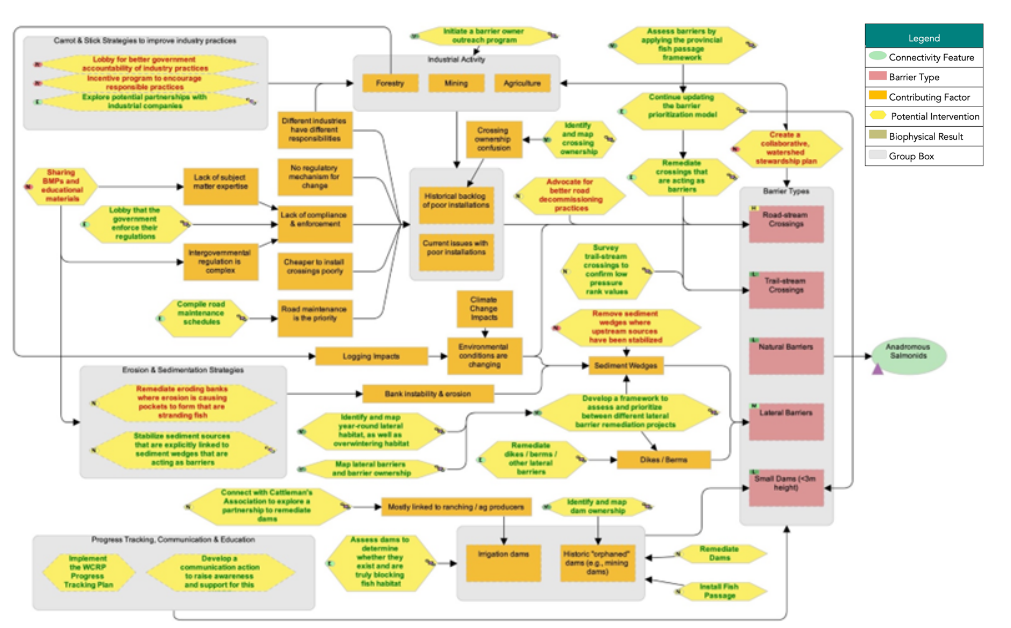
\includegraphics{content/images/situation-analysis.png}

}

\caption{\label{fig-sitan}SAMPLE Situation analysis developed by the
planning team to identify factors that contribute to fragmentation
(orange boxes), biophysical results (brown boxes), and potential
strategies/actions to improve connectivity (yellow hexagons) for target
species in the Horsefly River watershed.}

\end{figure}%

\section*{Strategies \& Actions}\label{strategies-actions}
\addcontentsline{toc}{section}{Strategies \& Actions}

\markright{Strategies \& Actions}

Effectiveness evaluation of identified conservation strategies and
associated actions to improve connectivity for target species in . The
planning team identified five broad strategies to implement through this
WCRP, 1) crossing remediation, 2) lateral barrier remediation, 3) dam
remediation, 4) barrier prevention, and 5) communication and education.
Individual actions were qualitatively evaluated based on the anticipated
effect each action will have on realizing on-the-ground gains in
connectivity. Effectiveness ratings are based on a combination of
``Feasibility and''Impact'', Feasibility is defined as the degree to
which the project team can implement the action within realistic
constraints (financial, time, ethical, etc.) and Impact is the degree to
which the action is likely to contribute to achieving one or more of the
goals established in this plan.

\section*{Strategy 1: Crossing
Remediation}\label{strategy-1-crossing-remediation}
\addcontentsline{toc}{section}{Strategy 1: Crossing Remediation}

\markright{Strategy 1: Crossing Remediation}

\begin{longtable}[]{@{}llllll@{}}

\caption{\label{tbl-S1}Strategy 1}

\tabularnewline

\caption{}\label{T_df614}\tabularnewline
\toprule\noalign{}
ID & Actions & Details & Feasibility & Impact & Effectiveness \\
\midrule\noalign{}
\endfirsthead
\toprule\noalign{}
ID & Actions & Details & Feasibility & Impact & Effectiveness \\
\midrule\noalign{}
\endhead
\bottomrule\noalign{}
\endlastfoot
1.1 & Remediate crossings that are acting as barriers & This action
represents some projects that would be led by the planning team with
conservation funds (e.g., orphaned barriers or those owned by
individuals), while other remediation projects would be the
responsibility of the barrier owner. Industry will have to be engaged to
successfully implement this intervention. PSC Southern Boundary
Restoration and Enhancement Fund proposal: - Complete remediation of one
priority barrier, including engineering designs HCTF proposal: -
Complete remediation of one priority barrier CNFASAR proposal (2022-26):
- Complete remediation of one priority barrier per year for four years
HRR Can help with finding local people to implement remediation
projects. & High & Very high & Effective \\
1.2 & Lobby that the government enforce their regulations & This can
apply to both provincial and federal governments. For example,
advocating for increased discretionary decisions to remove barriers to
fish. One action could be to submit barrier assessment data to show
proof that regulations are not being followed. & Very high & High &
Effective \\
1.3 & Initiate a barrier owner outreach program for locations on the
barrier remediation shortlist & Work with landowners / users (e.g., ATV
groups) to identify and remediate their aquatic barriers. Education
component can help prevent barriers in the first place. HRR to reach out
to owners of confirmed barriers to discuss remediation options; CWF to
reach out to provincial representatives. & Very high & Very high & Very
effective \\
1.4 & Knowledge Gap: Continue updating the barrier prioritization model
& The model has been updated to reflect 2021 field assessments and
intermediate barrier review. & Very high & High & Effective \\
1.5 & Knowledge Gap: conduct field assessments on updated preliminary
barrier list using the provincial fish passage framework and update
connectivity goal if additional barriers are added to the barrier
remediation shortlist & Twenty-six field assessments performed in 2021.
& Very high & Very high & Very effective \\
1.6 & Update longitudinal connectivity goal if additional barriers are
added to the barrier remediation shortlist & & & & \\
1.7 & Knowledge Gap: Identify and map crossing ownership & For barriers
on the barrier remediation shortlist. & Very high & Very high & Very
effective \\
1.8 & Knowledge Gap: Compile road maintenance schedules &
Ground-truthing is important, as the schedules do not always reflect
what happens in the field. & High & High & Effective \\
1.9 & Knowledge Gap: Survey trail-stream crossings to confirm low
pressure rating values & Need to access detailed trail maps in the
watershed to prioritize our time and resources. This should be
accomplished as people are out surveying for other reasons rather than
spending time and resources specifically to fill this knowledge gap.
CNFASAR proposal: Collaborate with WLFN to: - Develop field assessment
protocols for whether ATV trail stream crossings pass fish, and for
assessing other effects on fish habitat - Map potential trail-stream
crossings on salmon habitat that could be assessed - Assess 30-50 trail
stream crossings, record measurements, and take pictures & Very high &
Medium & Need more information \\
& & & & & \\

\end{longtable}

\section*{Strategy 2: Lateral Barrier
Remediation}\label{strategy-2-lateral-barrier-remediation}
\addcontentsline{toc}{section}{Strategy 2: Lateral Barrier Remediation}

\markright{Strategy 2: Lateral Barrier Remediation}

\begin{longtable}[]{@{}llllll@{}}

\caption{\label{tbl-S2}Strategy 2}

\tabularnewline

\caption{}\label{T_7f193}\tabularnewline
\toprule\noalign{}
ID & Actions & Details & Feasibility & Impact & Effectiveness \\
\midrule\noalign{}
\endfirsthead
\toprule\noalign{}
ID & Actions & Details & Feasibility & Impact & Effectiveness \\
\midrule\noalign{}
\endhead
\bottomrule\noalign{}
\endlastfoot
2.1 & Remediate dikes / berms / other lateral barriers & & High & Very
high & Effective \\
2.2 & Initiate a barrier owner outreach program & & Very high & Very
high & Very effective \\
2.3 & Knowledge Gap: Identify and map year-round lateral habitat, as
well as overwintering habitat & Explore the use of a drone to identify
lateral habitat. - Volunteers from the HRR will conduct field habitat
assessments following modules in the Pacific Streamkeepers Handbook to
assess disconnected lateral and overwintering salmon habitats in the
Horsefly watershed CNFASAR proposal: -Funding for equipment in
2022-2023, and for field transportation in 2022-2023, 2023-2024 & Very
high & Very high & Very effective \\
2.4 & Knowledge Gap: Map lateral barriers and barrier ownership & Focus
on identifying ownership of priority lateral barriers that we want to
remediate in the short-term. & Very high & Very high & Very effective \\
2.5 & Knowledge Gap: Develop a framework to assess and prioritize
between different lateral barrier remediation projects & CWF is leading
a provincial-scale analysis of the effect of rail lines on connectivity
for Anadromous Salmonids, as part of this project lateral habitat and
barrier assessments and prioritization methods will be developed. & Very
high & Very high & Very effective \\

\end{longtable}

\section*{Strategy 3: Dam Remediation}\label{strategy-3-dam-remediation}
\addcontentsline{toc}{section}{Strategy 3: Dam Remediation}

\markright{Strategy 3: Dam Remediation}

\begin{longtable}[]{@{}llllll@{}}

\caption{\label{tbl-S3}Strategy 3}

\tabularnewline

\caption{}\label{T_834a7}\tabularnewline
\toprule\noalign{}
ID & Actions & Details & Feasibility & Impact & Effectiveness \\
\midrule\noalign{}
\endfirsthead
\toprule\noalign{}
ID & Actions & Details & Feasibility & Impact & Effectiveness \\
\midrule\noalign{}
\endhead
\bottomrule\noalign{}
\endlastfoot
3.1 & Remediate Dams & & Medium & Very high & Need more information \\
3.2 & Install Fish Passage & & Medium & High & Need more information \\
3.3 & Connect with Cattleman\textquotesingle s Association to explore a
partnership to remediate dams & This may involve exploring alternative
water management actions that would allow for the remediation of
irrigation dams. & High & Medium & Need more information \\
3.4 & Knowledge Gap: Continue updating the barrier prioritization model
& The model has been updated to reflect 2021 field assessments and
intermediate barrier review. & Very high & High & Effective \\
3.5 & Knowledge Gap: Assess dams to determine whether they exist and are
truly blocking fish habitat & Four dams were assessed during 2021 field
season; additional field assessment needed. & Very high & High &
Effective \\
3.6 & Knowledge Gap: Identify and map dam ownership & & Very high & Very
high & Very effective \\

\end{longtable}

\section*{Strategy 4: Barrier
Prevention}\label{strategy-4-barrier-prevention}
\addcontentsline{toc}{section}{Strategy 4: Barrier Prevention}

\markright{Strategy 4: Barrier Prevention}

\begin{longtable}[]{@{}llllll@{}}

\caption{\label{tbl-S4}Strategy 4}

\tabularnewline

\caption{}\label{T_3e644}\tabularnewline
\toprule\noalign{}
ID & Actions & Details & Feasibility & Impact & Effectiveness \\
\midrule\noalign{}
\endfirsthead
\toprule\noalign{}
ID & Actions & Details & Feasibility & Impact & Effectiveness \\
\midrule\noalign{}
\endhead
\bottomrule\noalign{}
\endlastfoot
4.1 & Explore potential partnerships with industrial companies & Invite
industrial players to a workshop on how to apply crossing / lateral
barrier BMPs. BMPs could include those that minimize the need for
road-stream crossings. & Very high & High & Effective \\
4.2 & Stabilize sediment sources that are explicitly linked to sediment
wedges or erosion that are acting as barriers & This could include
numerous bank stabilization techniques, including restoring riparian
vegetation. This applies to some tributaries that have altered
confluence areas - the link needs to be made between confluence
alterations and timing of movement for juvenile fish. Local ranchers and
Cattleman\textquotesingle s association could be engaged, as well as
forestry licensees. & Very high & Medium & Need more information \\

\end{longtable}

\section*{Strategy 5: Communication and
Education}\label{strategy-5-communication-and-education}
\addcontentsline{toc}{section}{Strategy 5: Communication and Education}

\markright{Strategy 5: Communication and Education}

\begin{longtable}[]{@{}lll@{}}

\caption{\label{tbl-S5}Strategy 5}

\tabularnewline

\caption{}\label{T_06d55}\tabularnewline
\toprule\noalign{}
ID & Actions & Details \\
\midrule\noalign{}
\endfirsthead
\toprule\noalign{}
ID & Actions & Details \\
\midrule\noalign{}
\endhead
\bottomrule\noalign{}
\endlastfoot
5.1 & Implement the WCRP Progress Tracking Plan & The WCRP Progress
Tracking Plan will help the team determine if we are achieving our goals
and objectives. \\
5.2 & Develop a communication strategy to raise awareness and support
for this WCRP & This intervention includes communicating both the WCRP
and the collaborative process in developing it, as well as communicating
outcomes (e.g., barrier remediations). CNFASAR proposal: - HRR will work
with CWF to develop outreach and communications materials, including
press releases, social media content, a video, and content for their
website - With HRR, CWF will present on fish passage issues and
solutions at the annual Horsefly River Salmon Festival \\

\end{longtable}

\section*{Theories of Change \&
Objectives}\label{theories-of-change-objectives}
\addcontentsline{toc}{section}{Theories of Change \& Objectives}

\markright{Theories of Change \& Objectives}

Theories of Change are explicit assumptions around how the identified
actions will achieve gains in connectivity and contribute towards
reaching the goals of the plan. To develop Theories of Change, the
planning team developed explicit assumptions for each strategy which
helped to clarify the rationale used for undertaking actions and
provided an opportunity for feedback on invalid assumptions or missing
opportunities. The Theories of Change are results oriented and clearly
define the expected outcome. The following theory of change models were
developed by the WCRP planning team to ``map'' the causal (``if-then'')
progression of assumptions of how the actions within a strategy work
together to achieve project goals.

\begin{figure}

\centering{

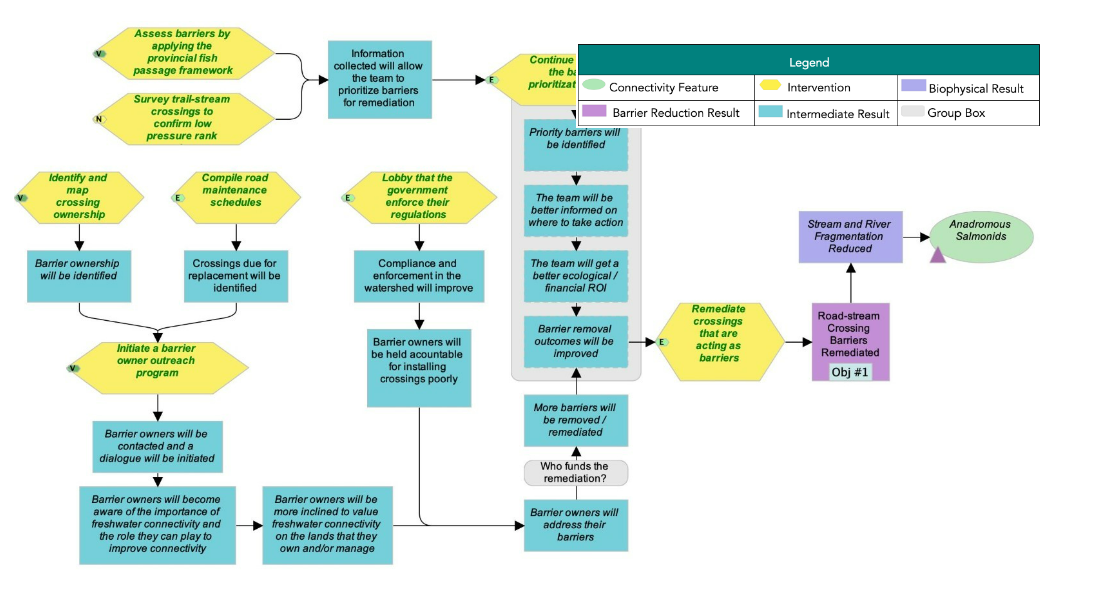
\includegraphics{content/images/flowchart-crossing-rem.png}

}

\caption{\label{fig-stra1}Theory of change developed by the planning
team for the actions identified under Strategy 1: Crossing Remediation
in the .}

\end{figure}%

\begin{figure}

\centering{

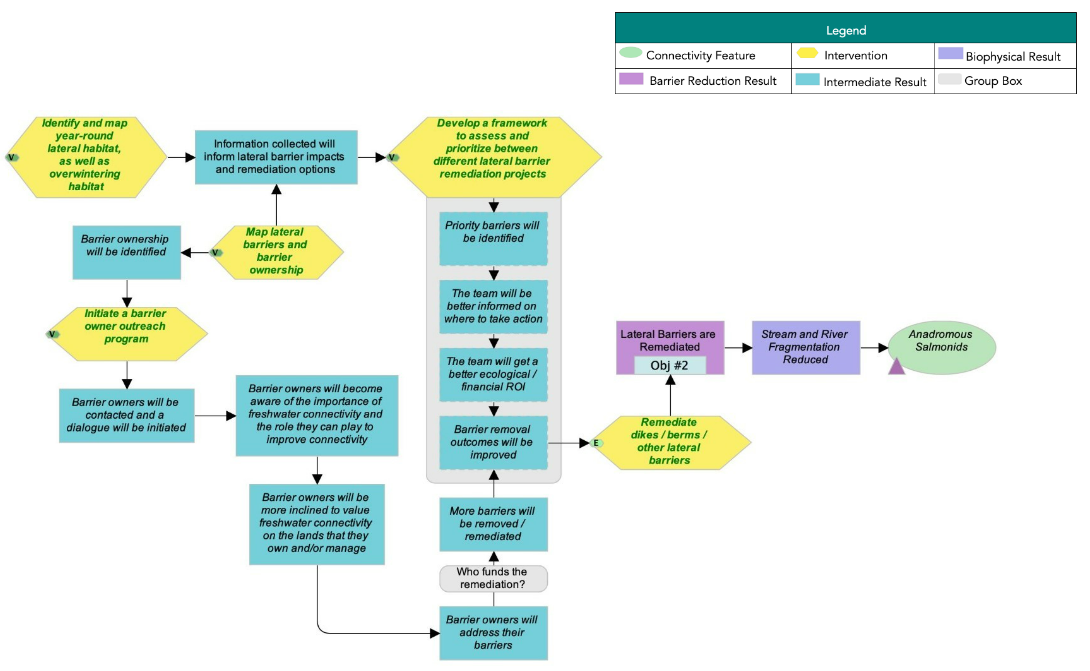
\includegraphics{content/images/flowchart-lat-bar-rem.png}

}

\caption{\label{fig-stra2}Theory of change developed by the planning
team for the actions identified under Strategy 2: Lateral Barrier
Remediation in .}

\end{figure}%

\begin{figure}

\centering{

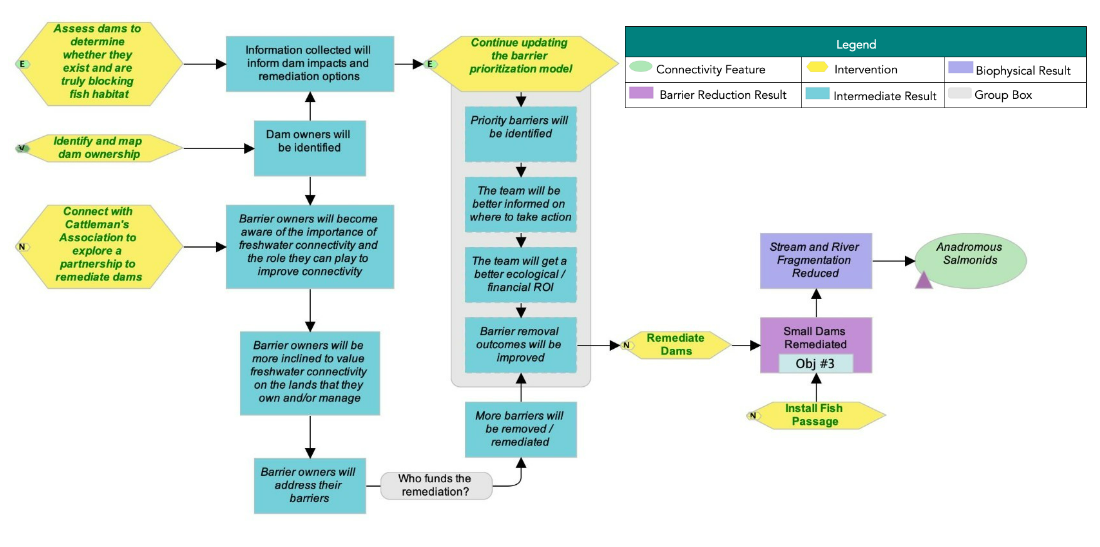
\includegraphics{content/images/flowchart-dam-rem.png}

}

\caption{\label{fig-stra3}Theory of change developed by the planning
team for the actions identified under Strategy 3: Dam Remediation in .}

\end{figure}%

\begin{figure}

\centering{

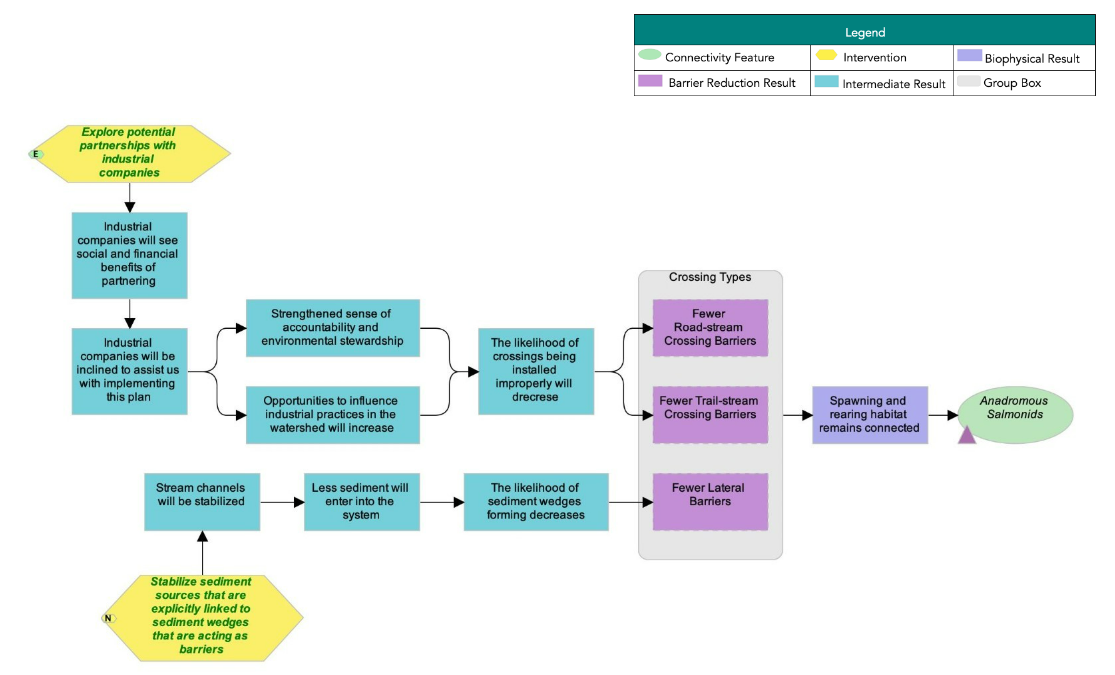
\includegraphics{content/images/flowchart-bar-prevent.png}

}

\caption{\label{fig-stra4}Theory of change developed by the planning
team for the actions identified under Strategy 4: Barrier Prevention in
.}

\end{figure}%

\section*{Operational Plan}\label{operational-plan-1}
\addcontentsline{toc}{section}{Operational Plan}

\markright{Operational Plan}

The operational plan represents a preliminary exercise undertaken by the
planning team to identify the potential leads, potential participants,
and estimated cost for the implementation of each action in . The table
below summarizes individuals, groups, or organizations that the planning
team felt could lead or participate in the implementation of the plan
and should be interpreted as the first step in on-going planning and
engagement to develop more detailed and sophisticated action plans for
each entry in the table. The individuals, groups, and organizations
listed under the ``Lead(s)'' or ``Potential Participants'' columns are
those that provisionally expressed interest in participating in one of
those roles or were suggested by the planning team for further
engagement (denoted in bold), for those that are not members of the
planning team. The leads, participants, and estimated costs in the
operational plan are not binding nor an official commitment of
resources, but rather provide a roadmap for future coordination and
engagement to work towards implementation of the WCRP.

\begin{longtable}[]{@{}llll@{}}

\caption{\label{tbl-opplan}Operational plan to support the
implementation of strategies and actions to improve connectivity for
target species in .}

\tabularnewline

\caption{}\label{T_a7f23}\tabularnewline
\toprule\noalign{}
Strategy / Actions & Lead(s) {[}1{]} & Participants3 & Total Budget \\
\midrule\noalign{}
\endfirsthead
\toprule\noalign{}
Strategy / Actions & Lead(s) {[}1{]} & Participants3 & Total Budget \\
\midrule\noalign{}
\endhead
\bottomrule\noalign{}
\endlastfoot
Strategy 1: Crossing Remediation & & & \$3,666,300.00 \\
1.1 -- Remediate crossings that are acting as barriers & CWF & Horsefly
River Roundtable, Fisheries and Oceans Canada (DFO) & \$3,500,000.00 \\
1.2 -- Lobby that the government enforce their regulations & TBD & CWF,
Horsefly River Roundtable, Williams Lake First Nation (WLFN) &
\$10,000.00 \\
1.3 -- Initiate a barrier owner outreach program for locations on the
barrier remediation shortlist & HRR, CWF, DFO & & TBD \\
1.4 -- Knowledge Gap: Continue updating the barrier prioritization model
& CWF & TBD & \$100,000.00 \\
1.5 -- Knowledge Gap: conduct field assessments on updated preliminary
barrier list using the provincial fish passage framework and update
connectivity goal if additional barriers are added to the barrier
remediation shortlist & CWF & Horsefly River Roundtable, DFO &
\$50,300.00 \\
1.6 - Update longitudinal connectivity goal if additional barriers are
added to the barrier remediation shortlist & & & \\
1.7 -- Knowledge Gap: Identify and map crossing ownership for barriers
on the barrier remediation shortlist & TBD & CWF, DFO (Anthonie) &
\$1,500.00 \\
1.8 -- Knowledge Gap: Compile road maintenance schedules & DFO & CWF,
WLFN, DFO, FLNRORD & \$2,000.00 \\
1.9 -- Knowledge Gap: Survey trail-stream crossings to confirm low
pressure rating values & WLFN & CWF, DFO & \$2,500.00 \\
Strategy 2: Lateral Barrier Remediation & & & \$80,000.00 \\
2.1 -- Remediate dikes / berms / other structures that are acting as
barriers & CWF & DFO, Horsefly River Roundtable & TBD \\
2.2 -- Initiate a barrier owner outreach program & TBD & CWF, DFO &
TBD \\
2.3 -- Knowledge Gap: Identify and map year-round lateral habitat, as
well as overwintering habitat & Horsefly River Roundtable, DFO & CWF,
Northern Shuswap Tribal Council (NSTC), WLFN & \$65,000.00 \\
2.4 -- Knowledge Gap: Map lateral barriers and barrier ownership & CWF &
DFO, Horsefly River Roundtable & \$5,000.00 \\
2.5 -- Knowledge Gap: Develop a framework to assess and prioritize
between different lateral barrier remediation projects & CWF & DFO &
\$10,000.00 \\
Strategy 3: Dam Remediation & & & \$1,305,000.00 \\
3.1 - Remediate Dams & TBD & TBD & \$1,305,000.00 \\
3.2 - Install Fish Passage & TBD & TBD & TBD \\
3.3 - Connect with Cattleman\textquotesingle s Association to explore a
partnership to remediate dams & TBD & TBD & TBD \\
3.4 - Knowledge Gap: Continue updating the barrier prioritization model
& CWF & TBD & \$0.00 \\
3.5 - Knowledge Gap: Assess dams to determine whether they exist and are
truly blocking salmon habitat & HRR(?) DFO(?) CWF(?) & TBD & TBD \\
3.6 - Knowledge Gap: Identify and map dam ownership & TBD & TBD & TBD \\
Strategy 4: Barrier Prevention & & & \$110,000.00 \\
4.1 -- Explore potential partnerships with industrial companies & TBD &
CWF, DFO, Horsefly River Roundtable, WLFN & \$10,000.00 \\
4.2 -- Stabilize sediment sources that are explicitly linked to sediment
wedges or erosion that are acting as barriers & TBD & DFO &
\$100,000.00 \\
Strategy 5: Progress Tracking Plan & & & TBD \\
5.1 - Implement the WCRP Progress Tracking Plan & CWF & & TBD \\
5.2 - Develop a communication action to raise awareness and support for
this WCRP & CWF, HRR & TBD & TBD \\
Total: & & & \$5,161,300.00 \\
Fundraising total: & & & \$2,508,800 \\
Proponent/government contribution total: & & & \$2,652,500 \\

\end{longtable}

\section*{Funding Sources}\label{funding-sources}
\addcontentsline{toc}{section}{Funding Sources}

\markright{Funding Sources}

\global\setlength{\Oldarrayrulewidth}{\arrayrulewidth}

\global\setlength{\Oldtabcolsep}{\tabcolsep}

\setlength{\tabcolsep}{2pt}

\renewcommand*{\arraystretch}{1.5}



\providecommand{\ascline}[3]{\noalign{\global\arrayrulewidth #1}\arrayrulecolor[HTML]{#2}\cline{#3}}

\begin{longtable}[c]{|p{5.52in}|p{60.28in}}

\caption{\label{tbl-fund}Potential funding sources for plan
implementation in . The Canadian Wildlife Federation and the planning
team can coordinate proposal submission through these sources.}

\tabularnewline

\hhline{>{\arrayrulecolor[HTML]{666666}\global\arrayrulewidth=1.5pt}->{\arrayrulecolor[HTML]{666666}\global\arrayrulewidth=1.5pt}-}

\multicolumn{1}{>{\cellcolor[HTML]{008270}\raggedright}m{\dimexpr 5.52in+0\tabcolsep}}{\textcolor[HTML]{FFFFFF}{\fontsize{11}{11}\selectfont{\global\setmainfont{Arial}{Funding\ Source}}}} & \multicolumn{1}{>{\cellcolor[HTML]{008270}\raggedright}m{\dimexpr 60.28in+0\tabcolsep}}{\textcolor[HTML]{FFFFFF}{\fontsize{11}{11}\selectfont{\global\setmainfont{Arial}{Spending\ Restrictions\ and\ Other\ Consideration}}}} \\

\noalign{\global\arrayrulewidth 0pt}\arrayrulecolor[HTML]{000000}

\hhline{>{\arrayrulecolor[HTML]{666666}\global\arrayrulewidth=1.5pt}->{\arrayrulecolor[HTML]{666666}\global\arrayrulewidth=1.5pt}-}\endfirsthead 

\hhline{>{\arrayrulecolor[HTML]{666666}\global\arrayrulewidth=1.5pt}->{\arrayrulecolor[HTML]{666666}\global\arrayrulewidth=1.5pt}-}

\multicolumn{1}{>{\cellcolor[HTML]{008270}\raggedright}m{\dimexpr 5.52in+0\tabcolsep}}{\textcolor[HTML]{FFFFFF}{\fontsize{11}{11}\selectfont{\global\setmainfont{Arial}{Funding\ Source}}}} & \multicolumn{1}{>{\cellcolor[HTML]{008270}\raggedright}m{\dimexpr 60.28in+0\tabcolsep}}{\textcolor[HTML]{FFFFFF}{\fontsize{11}{11}\selectfont{\global\setmainfont{Arial}{Spending\ Restrictions\ and\ Other\ Consideration}}}} \\

\noalign{\global\arrayrulewidth 0pt}\arrayrulecolor[HTML]{000000}

\hhline{>{\arrayrulecolor[HTML]{666666}\global\arrayrulewidth=1.5pt}->{\arrayrulecolor[HTML]{666666}\global\arrayrulewidth=1.5pt}-}\endhead



\multicolumn{1}{>{\raggedright}m{\dimexpr 5.52in+0\tabcolsep}}{\textcolor[HTML]{000000}{\fontsize{11}{11}\selectfont{\global\setmainfont{Arial}{Land\ Based\ Investment\ Strategy}}}} & \multicolumn{1}{>{\raggedright}m{\dimexpr 60.28in+0\tabcolsep}}{\textcolor[HTML]{000000}{\fontsize{11}{11}\selectfont{\global\setmainfont{Arial}{Assessment\ and\ remediation\ of\ fish\ passage\ using\ provincial\ strategic\ approach.\ Primarily\ for\ remediation\ of\ Ministry-owned/orphaned\ barriers\ on\ forest\ service\ roads.}}}} \\

\noalign{\global\arrayrulewidth 0pt}\arrayrulecolor[HTML]{000000}





\multicolumn{1}{>{\raggedright}m{\dimexpr 5.52in+0\tabcolsep}}{\textcolor[HTML]{000000}{\fontsize{11}{11}\selectfont{\global\setmainfont{Arial}{Environmental\ Enhancement\ Fund}}}} & \multicolumn{1}{>{\raggedright}m{\dimexpr 60.28in+0\tabcolsep}}{\textcolor[HTML]{000000}{\fontsize{11}{11}\selectfont{\global\setmainfont{Arial}{Fish\ and\ wildlife\ passage\ improvements\ and\ restoration\ at\ stream\ and\ animal\ crossings\ at\ MOTI\ roads\ including\ culvert\ retrofits\ and\ replacement\ to\ restore\ Pacific\ salmon\ and\ trout\ access,\ and\ wildlife\ tunnels.\ Primarily\ for\ crossings\ linked\ to\ highway\ infrastructure.}}}} \\

\noalign{\global\arrayrulewidth 0pt}\arrayrulecolor[HTML]{000000}





\multicolumn{1}{>{\raggedright}m{\dimexpr 5.52in+0\tabcolsep}}{\textcolor[HTML]{000000}{\fontsize{11}{11}\selectfont{\global\setmainfont{Arial}{Community\ Salmon\ Program}}}} & \multicolumn{1}{>{\raggedright}m{\dimexpr 60.28in+0\tabcolsep}}{\textcolor[HTML]{000000}{\fontsize{11}{11}\selectfont{\global\setmainfont{Arial}{For\ projects\ supporting\ the\ protection,\ conservation\ and\ enhancement\ or\ rehabilitation\ of\ Pacific\ salmonids\ and\ their\ habitat.\ Funding\ for\ volunteer\ and\ not-for-profit\ community-based\ groups.\ Applicant\ must\ have\ a\ significant\ volunteer\ component\ to\ their\ group\ and\ to\ the\ project.\ Requires\ 50\%\ match\ for\ funding\ (volunteer,\ in-kind,\ donation\ or\ other\ grants).\ }}}} \\

\noalign{\global\arrayrulewidth 0pt}\arrayrulecolor[HTML]{000000}





\multicolumn{1}{>{\raggedright}m{\dimexpr 5.52in+0\tabcolsep}}{\textcolor[HTML]{000000}{\fontsize{11}{11}\selectfont{\global\setmainfont{Arial}{Southern\ Boundary\ Restoration\ and\ Enhancement\ Fund}}}} & \multicolumn{1}{>{\raggedright}m{\dimexpr 60.28in+0\tabcolsep}}{\textcolor[HTML]{000000}{\fontsize{11}{11}\selectfont{\global\setmainfont{Arial}{Supports\ 3\ activities:\ (1)\ develop\ improved\ information\ for\ resource\ management;\ (2)\ Rehabilitate\ and\ restore\ marine\ and\ freshwater\ habitat;\ and\ (3)\ enhance\ wild\ stock\ production\ through\ low\ technology\ techniques.\ Emphasis\ for\ funding\ is\ on\ stocks\ of\ conservation\ concern,\ particularly\ those\ contributing\ to\ a\ fishery\ and\ stocks\ of\ bilateral\ fishery\ relevance.}}}} \\

\noalign{\global\arrayrulewidth 0pt}\arrayrulecolor[HTML]{000000}





\multicolumn{1}{>{\raggedright}m{\dimexpr 5.52in+0\tabcolsep}}{\textcolor[HTML]{000000}{\fontsize{11}{11}\selectfont{\global\setmainfont{Arial}{Habitat\ Conservation\ Trust\ Foundation\ Enhancement\ and\ Restoration\ Grants}}}} & \multicolumn{1}{>{\raggedright}m{\dimexpr 60.28in+0\tabcolsep}}{\textcolor[HTML]{000000}{\fontsize{11}{11}\selectfont{\global\setmainfont{Arial}{Projects\ that\ focus\ on\ freshwater\ wild\ fish,\ native\ wildlife\ species\ and\ their\ habitats,\ have\ the\ potential\ to\ achieve\ a\ significant\ conservation\ outcome,\ while\ maintaining\ or\ enhancing\ opportunities\ for\ fishing,\ hunting,\ trapping,\ wildlife\ viewing\ and\ associated\ outdoor\ recreational\ activities.\ Primary\ focus\ is\ on\ provincially\ managed\ fisheries\ such\ as\ Steelhead\ and\ Westslope\ Cutthroat\ Trout.\ Requires\ 50\%\ funding\ match.}}}} \\

\noalign{\global\arrayrulewidth 0pt}\arrayrulecolor[HTML]{000000}





\multicolumn{1}{>{\raggedright}m{\dimexpr 5.52in+0\tabcolsep}}{\textcolor[HTML]{000000}{\fontsize{11}{11}\selectfont{\global\setmainfont{Arial}{Environmental\ Damages\ Fund}}}} & \multicolumn{1}{>{\raggedright}m{\dimexpr 60.28in+0\tabcolsep}}{\textcolor[HTML]{000000}{\fontsize{11}{11}\selectfont{\global\setmainfont{Arial}{Direct\ funds\ received\ from\ fines,\ court\ orders\ and\ voluntary\ payments\ to\ priority\ projects\ that\ will\ benefit\ Canada’s\ natural\ environment,\ under\ 4\ categories\ of\ improvement\ (in\ order\ of\ preference):\ (1)\ restoration,\ (2)\ environmental\ quality\ improvement,\ (3)\ research\ and\ development,\ and\ (4)\ education\ and\ awareness.}}}} \\

\noalign{\global\arrayrulewidth 0pt}\arrayrulecolor[HTML]{000000}





\multicolumn{1}{>{\raggedright}m{\dimexpr 5.52in+0\tabcolsep}}{\textcolor[HTML]{000000}{\fontsize{11}{11}\selectfont{\global\setmainfont{Arial}{Habitat\ Stewardship\ Program\ for\ Aquatic\ Species\ at\ Risk}}}} & \multicolumn{1}{>{\raggedright}m{\dimexpr 60.28in+0\tabcolsep}}{\textcolor[HTML]{000000}{\fontsize{11}{11}\selectfont{\global\setmainfont{Arial}{Program\ for\ non-profits,\ Indigenous\ governments,\ academic\ institutions\ for\ activities\ that\ align\ with\ recovery\ actions\ identified\ in\ SARA\ recovery\ documents\ and/or\ COSEWIC\ assessment\ documents.\ Project\ must\ address\ one\ or\ more\ of\ 3\ broad\ categories:\ (1)\ Important\ habitat\ for\ aquatic\ species\ at\ risk\ is\ improved\ and/or\ managed\ to\ meet\ their\ recovery\ needs;\ (2)\ Threats\ to\ aquatic\ species\ at\ risk\ and/or\ their\ habitat\ are\ stopped,\ removed,\ and/or\ mitigated;\ (3)\ Collaboration\ and\ partnerships\ support\ the\ conservation\ and\ recovery\ of\ aquatic\ species\ at\ risk.\ Limited\ to\ at-risk\ species\ listed\ under\ COSEWIC\ and/or\ SARA\ as\ threatened,\ endangered\ or\ special\ concern.\ }}}} \\

\noalign{\global\arrayrulewidth 0pt}\arrayrulecolor[HTML]{000000}





\multicolumn{1}{>{\raggedright}m{\dimexpr 5.52in+0\tabcolsep}}{\textcolor[HTML]{000000}{\fontsize{11}{11}\selectfont{\global\setmainfont{Arial}{Canada\ Nature\ Fund\ for\ Aquatic\ Species\ at\ Risk}}}} & \multicolumn{1}{>{\raggedright}m{\dimexpr 60.28in+0\tabcolsep}}{\textcolor[HTML]{000000}{\fontsize{11}{11}\selectfont{\global\setmainfont{Arial}{Funding\ program\ aimed\ at\ addressing\ priority\ threats\ for\ aquatic\ species\ at\ risk\ listed\ as\ endangered,\ threatened\ or\ Special\ Concern\ by\ COSEWIC,\ as\ they\ align\ with\ existing\ federal,\ provincial\ or\ other\ local\ recovery\ plans.\ Limited\ to\ species\ in\ the\ Columbia\ and\ Fraser\ basins\ in\ BC,\ among\ other\ priority\ areas\ across\ Canada.\ Focus\ on\ multi-year,\ multi-partner\ initiatives\ that\ apply\ an\ ecosystem\ or\ multi-species\ approach\ and\ create\ a\ legacy\ by\ enabling\ recovery\ actions\ that\ carry\ beyond\ the\ life\ of\ the\ funding\ program.\ Amounts\ from\ \$100K-\$1M\ available\ per\ year.}}}} \\

\noalign{\global\arrayrulewidth 0pt}\arrayrulecolor[HTML]{000000}





\multicolumn{1}{>{\raggedright}m{\dimexpr 5.52in+0\tabcolsep}}{\textcolor[HTML]{000000}{\fontsize{11}{11}\selectfont{\global\setmainfont{Arial}{BC\ Salmon\ Restoration\ and\ Innovation\ Fund}}}} & \multicolumn{1}{>{\raggedright}m{\dimexpr 60.28in+0\tabcolsep}}{\textcolor[HTML]{000000}{\fontsize{11}{11}\selectfont{\global\setmainfont{Arial}{Funding\ for\ Indigenous\ enterprises,\ academia,\ industry\ associations,\ stewardship\ groups\ and\ commercial\ groups\ to\ support\ initiatives\ that\ support\ the\ protection\ and\ restoration\ of\ wild\ Pacific\ salmon\ and\ other\ BC\ fish\ stocks\ or\ ensure\ fish\ and\ seafood\ sector\ in\ BC\ is\ environmentally\ and\ economically\ sustainable.\ Five\ main\ priorities\ including\ species\ of\ concern\ rebuilding\ through\ habitat\ restoration\ with\ priority\ for\ projects\ that\ are\ part\ of\ a\ watershed-scale\ restoration\ plan/prioritization\ effort;\ build\ on\ successful\ previous\ restoration\ efforts;\ focus\ on\ critical\ habitat\ and/or\ the\ rehabilitation\ of\ natural\ ecosystem\ processes.}}}} \\

\noalign{\global\arrayrulewidth 0pt}\arrayrulecolor[HTML]{000000}





\multicolumn{1}{>{\raggedright}m{\dimexpr 5.52in+0\tabcolsep}}{\textcolor[HTML]{000000}{\fontsize{11}{11}\selectfont{\global\setmainfont{Arial}{Aboriginal\ Fund\ for\ Species\ at\ Risk}}}} & \multicolumn{1}{>{\raggedright}m{\dimexpr 60.28in+0\tabcolsep}}{\textcolor[HTML]{000000}{\fontsize{11}{11}\selectfont{\global\setmainfont{Arial}{Program\ for\ Indigenous\ groups\ for\ activities\ that\ align\ with\ recovery\ actions\ identified\ in\ SARA\ recovery\ documents\ and/or\ COSEWIC\ assessment\ documents\ for\ species\ listed\ as\ Endangered,\ Threatened,\ or\ Special\ Concern\ by\ SARA\ or\ COSEWIC.\ Project\ must\ address\ one\ or\ more\ of\ 4\ broad\ categories:\ (1)\ Habitat\ for\ species\ at\ risk\ is\ improved\ and/or\ managed\ to\ meet\ their\ recovery\ needs;\ (2)\ Threats\ to\ species\ at\ risk\ and/or\ their\ habitat\ are\ stopped,\ removed\ and/or\ mitigated;\ (3)\ Collaboration,\ information\ sharing\ and\ partnership\ between\ Indigenous\ communities,\ governments\ and\ organizations\ and\ other\ interested\ parties\ (e.g.\ federal/provincial/territorial\ governments,\ academia,\ industry,\ private\ sector)\ is\ enhanced;\ and\ (4)\ Capacity\ within\ Indigenous\ communities,\ to\ lead\ in\ the\ stewardship\ of\ species\ at\ risk\ and\ contribute\ to\ broader\ SARA\ implementation,\ is\ strengthened.\ }}}} \\

\noalign{\global\arrayrulewidth 0pt}\arrayrulecolor[HTML]{000000}





\multicolumn{1}{>{\raggedright}m{\dimexpr 5.52in+0\tabcolsep}}{\textcolor[HTML]{000000}{\fontsize{11}{11}\selectfont{\global\setmainfont{Arial}{Federal\ Gas\ Tax\ Fund\ -\ Community\ Works\ Fund}}}} & \multicolumn{1}{>{\raggedright}m{\dimexpr 60.28in+0\tabcolsep}}{\textcolor[HTML]{000000}{\fontsize{11}{11}\selectfont{\global\setmainfont{Arial}{Funding\ available\ to\ local\ governments\ from\ federal\ gas\ tax,\ with\ funds\ to\ be\ allocated\ for\ a\ variety\ of\ municipal\ projects/initiatives,\ including\ local\ roads/bridges\ and\ disaster\ mitigation.}}}} \\

\noalign{\global\arrayrulewidth 0pt}\arrayrulecolor[HTML]{000000}





\multicolumn{1}{>{\raggedright}m{\dimexpr 5.52in+0\tabcolsep}}{\textcolor[HTML]{000000}{\fontsize{11}{11}\selectfont{\global\setmainfont{Arial}{Disaster\ Mitigation\ and\ Adaptation\ Fund}}}} & \multicolumn{1}{>{\raggedright}m{\dimexpr 60.28in+0\tabcolsep}}{\textcolor[HTML]{000000}{\fontsize{11}{11}\selectfont{\global\setmainfont{Arial}{For\ those\ projects\ where\ flood\ risk\ is\ high:\ Funding\ available\ to\ local,\ regional\ and\ provincial\ governments,\ private\ sector,\ non-profit\ organizations,\ and\ Indigenous\ groups\ for\ projects\ aimed\ at\ reducing\ the\ socio-economic,\ environmental\ and\ cultural\ impacts\ triggered\ by\ natural\ hazards\ and\ extreme\ weather\ events\ and\ taking\ into\ consideration\ current\ and\ future\ impacts\ of\ climate\ change\ in\ communities\ and\ infrastructure\ at\ high\ risk.\ Includes\ both\ new\ construction\ of\ public\ infrastructure\ and\ modification/reinforcement\ of\ existing\ infrastructure.\ Projects\ must\ have\ a\ minimum\ of\ \$20\ M\ in\ eligible\ expenditures\ and\ can\ be\ bundled\ together.}}}} \\

\noalign{\global\arrayrulewidth 0pt}\arrayrulecolor[HTML]{000000}





\multicolumn{1}{>{\raggedright}m{\dimexpr 5.52in+0\tabcolsep}}{\textcolor[HTML]{000000}{\fontsize{11}{11}\selectfont{\global\setmainfont{Arial}{Community\ Gaming\ Grants}}}} & \multicolumn{1}{>{\raggedright}m{\dimexpr 60.28in+0\tabcolsep}}{\textcolor[HTML]{000000}{\fontsize{11}{11}\selectfont{\global\setmainfont{Arial}{Funding\ for\ non-profit\ organizations\ (check\ funding\ program\ guidelines\ for\ specific\ eligibility\ requirements)\ for\ programs\ that\ help\ to\ protect\ and\ improve\ the\ environment\ by:\ (1)\ Conserving\ or\ revitalizing\ local\ ecosystems,\ (2)\ Reducing\ greenhouse\ gas\ emissions,\ (3)\ Providing\ community\ education\ or\ engagement\ opportunities\ related\ to\ the\ environment\ and\ agriculture\ or\ (4)\ Supporting\ the\ welfare\ of\ domestic\ animals\ and/or\ wildlife.\ Grants\ range\ from\ \$100K-250K\ per\ year.}}}} \\

\noalign{\global\arrayrulewidth 0pt}\arrayrulecolor[HTML]{000000}





\multicolumn{1}{>{\raggedright}m{\dimexpr 5.52in+0\tabcolsep}}{\textcolor[HTML]{000000}{\fontsize{11}{11}\selectfont{\global\setmainfont{Arial}{Sitka\ Foundation}}}} & \multicolumn{1}{>{\raggedright}m{\dimexpr 60.28in+0\tabcolsep}}{\textcolor[HTML]{000000}{\fontsize{11}{11}\selectfont{\global\setmainfont{Arial}{Funding\ for\ registered\ charities,\ universities,\ and\ government\ agencies\ (qualified\ Canadian\ organizations)\ for\ projects\ related\ to\ coastline\ and\ watershed\ conservation\ and\ climate\ change\ in\ 4\ key\ areas:\ (1)\ land,\ water,\ and\ ocean\ conservation,\ (2)\ scientific\ research\ for\ nature\ and\ the\ environment,\ (3)\ \ public\ engagement\ around\ the\ importance\ of\ a\ healthy\ environment,\ (4)\ innovative\ conservation\ efforts\ in\ Canadian\ communities,\ at\ the\ local,\ provincial,\ and\ federal\ levels}}}} \\

\noalign{\global\arrayrulewidth 0pt}\arrayrulecolor[HTML]{000000}





\multicolumn{1}{>{\raggedright}m{\dimexpr 5.52in+0\tabcolsep}}{\textcolor[HTML]{000000}{\fontsize{11}{11}\selectfont{\global\setmainfont{Arial}{TULA\ Foundation}}}} & \multicolumn{1}{>{\raggedright}m{\dimexpr 60.28in+0\tabcolsep}}{\textcolor[HTML]{000000}{\fontsize{11}{11}\selectfont{\global\setmainfont{Arial}{Supports\ various\ environmental\ programs\ of\ interest\ to\ the\ Foundation\ on\ a\ case-by-case\ basis.}}}} \\

\noalign{\global\arrayrulewidth 0pt}\arrayrulecolor[HTML]{000000}





\multicolumn{1}{>{\raggedright}m{\dimexpr 5.52in+0\tabcolsep}}{\textcolor[HTML]{000000}{\fontsize{11}{11}\selectfont{\global\setmainfont{Arial}{Vancouver\ Foundation}}}} & \multicolumn{1}{>{\raggedright}m{\dimexpr 60.28in+0\tabcolsep}}{\textcolor[HTML]{000000}{\fontsize{11}{11}\selectfont{\global\setmainfont{Arial}{Granting\ agency\ for\ community,\ social\ and\ environmental\ initiatives\ for\ qualified\ Canadian\ organizations\ (charitable\ organizations,\ universities,\ government\ agencies).\ Granting\ programs\ change\ on\ an\ annual\ basis.}}}} \\

\noalign{\global\arrayrulewidth 0pt}\arrayrulecolor[HTML]{000000}





\multicolumn{1}{>{\raggedright}m{\dimexpr 5.52in+0\tabcolsep}}{\textcolor[HTML]{000000}{\fontsize{11}{11}\selectfont{\global\setmainfont{Arial}{BC\ Conservation\ Foundation\ Small\ Project\ Fund}}}} & \multicolumn{1}{>{\raggedright}m{\dimexpr 60.28in+0\tabcolsep}}{\textcolor[HTML]{000000}{\fontsize{11}{11}\selectfont{\global\setmainfont{Arial}{Funding\ available\ to\ Non-profits,\ fish\ and\ wildlife\ clubs\ (sportsmen’s\ associations),\ businesses,\ local/regional\ governments,\ public\ organizations\ and\ First\ Nations\ for\ projects\ with\ demonstrated\ positive\ impact\ for\ fish,\ wildlife\ and\ habitat,\ including\ outreach\ programs.\ Preference\ given\ to\ projects\ where\ BCCF\ is\ not\ the\ sole\ funder.}}}} \\

\noalign{\global\arrayrulewidth 0pt}\arrayrulecolor[HTML]{000000}





\multicolumn{1}{>{\raggedright}m{\dimexpr 5.52in+0\tabcolsep}}{\textcolor[HTML]{000000}{\fontsize{11}{11}\selectfont{\global\setmainfont{Arial}{Real\ Estate\ Foundation\ of\ BC\ General\ Grants}}}} & \multicolumn{1}{>{\raggedright}m{\dimexpr 60.28in+0\tabcolsep}}{\textcolor[HTML]{000000}{\fontsize{11}{11}\selectfont{\global\setmainfont{Arial}{Funding\ for\ First\ Nations,\ charities\ and\ societies,\ non-governmental\ organizations,\ universities\ and\ colleges,\ trade\ associations,\ local\ and\ regional\ governments,\ and\ social\ enterprises\ registered\ as\ C3s\ for\ sustainable\ land\ use\ and\ real\ estate\ practices\ in\ BC.\ Funds\ up\ to\ 50\%\ of\ cash\ portion\ of\ a\ project.}}}} \\

\noalign{\global\arrayrulewidth 0pt}\arrayrulecolor[HTML]{000000}

\hhline{>{\arrayrulecolor[HTML]{666666}\global\arrayrulewidth=1.5pt}->{\arrayrulecolor[HTML]{666666}\global\arrayrulewidth=1.5pt}-}


\end{longtable}

\arrayrulecolor[HTML]{000000}

\global\setlength{\arrayrulewidth}{\Oldarrayrulewidth}

\global\setlength{\tabcolsep}{\Oldtabcolsep}

\renewcommand*{\arraystretch}{1}

\chapter*{Data Download and Methods}\label{data-download-and-methods}
\addcontentsline{toc}{chapter}{Data Download and Methods}

\markboth{Data Download and Methods}{Data Download and Methods}

\section*{Appendix A: Modelled Anadromous Salmon Habitat
Maps}\label{appendix-a-modelled-anadromous-salmon-habitat-maps}
\addcontentsline{toc}{section}{Appendix A: Modelled Anadromous Salmon
Habitat Maps}

\markright{Appendix A: Modelled Anadromous Salmon Habitat Maps}

SAMPLE High-resolution PDF maps of the Quesnel-Bowron watershed and
model results can be accessed
\href{https://github.com/smnorris/bcfishpass/tree/main/wcrp/pdfs}{here}.
The watershed is divided into multiple maps sheets to allow for detailed
examination of modelled spawning and rearing habitat and priority
barriers identified through this planning process. The locations of WCRP
priority barriers and associated map sheet numbers are shown below. In
each individual map sheet, priority barriers are symbolized using the
following notation:

\begin{figure}

\centering{

\includegraphics{content/images/overview-map-ques-bow.png}

}

\caption{\label{fig-over}Quesnel-Bowron watershed overview map
identifying the portions of the watershed covered by each map sheet
(grey squares) and the prioritized barriers on the intermediate barrier
list (orange points; see Appendix C).}

\end{figure}%

\section*{Appendix B: Connectivity Status Assessment
Methods}\label{appendix-b-connectivity-status-assessment-methods}
\addcontentsline{toc}{section}{Appendix B: Connectivity Status
Assessment Methods}

\markright{Appendix B: Connectivity Status Assessment Methods}

SAMPLE The connectivity status assessment for anadromous salmonids in
the Bulkley River watershed builds on existing connectivity modelling
work undertaken by the BC Fish Passage Technical Working Group,
resulting in a flexible, customizable open-source spatial model called
\href{https://github.com/smnorris/bcfishpass}{``bcfishpass''}. The model
spatially locates known and modelled barriers to fish passage,
identifies potential spawning and rearing habitat for target species,
and estimates the amount of habitat that is currently accessible to
target species. The model uses an adapted version of the Intrinsic
Potential (IP) fish habitat modelling framework (see Sheer et al. (2009)
for an overview of the IP framework). The habitat model uses two
geomorphic characteristics of the stream network --- channel gradient
and mean annual discharge --- to identify potential spawning habitat and
rearing habitat for each target species. The habitat model does not
attempt to definitively map each habitat type nor estimate habitat
quality, but rather identifies stream segments that have high potential
to support spawning or rearing habitat for each species based on the
geomorphic characteristics of the segment. For more details on the
connectivity and habitat model structure and parameters, please see
Mazany-Wright, Norris, et al. (2021a). The variables and thresholds used
to model potential spawning and rearing habitat for each target species
are summarized in Table 15. The quantity of modelled habitat for each
species was aggregated for each habitat type to inform the two KEAs ---
Accessible Spawning Habitat and Accessible Rearing Habitat --- and
represents a linear measure of potential habitat. To recognize the
rearing value provided by features represented by polygons for certain
species (e.g., wetlands for Coho Salmon and lakes for Sockeye Salmon) a
multiplier of 1.5x the length of the stream segments flowing through the
polygons was applied.

\global\setlength{\Oldarrayrulewidth}{\arrayrulewidth}

\global\setlength{\Oldtabcolsep}{\tabcolsep}

\setlength{\tabcolsep}{2pt}

\renewcommand*{\arraystretch}{1.5}



\providecommand{\ascline}[3]{\noalign{\global\arrayrulewidth #1}\arrayrulecolor[HTML]{#2}\cline{#3}}

\begin{longtable}[c]{|p{1.43in}|p{3.34in}|p{8.40in}|p{3.09in}|p{3.03in}|p{1.94in}|p{1.33in}}

\caption{\label{tbl-param}Additional Key Actors. Key Actors are the
individuals, groups, and/or organizations, outside of the planning team,
with influence and relevant experience in the watershed, whose
engagement will be critical for the successful implementation of the
Quesnel-Bowron watershed}

\tabularnewline

\hhline{>{\arrayrulecolor[HTML]{666666}\global\arrayrulewidth=1.5pt}->{\arrayrulecolor[HTML]{666666}\global\arrayrulewidth=1.5pt}->{\arrayrulecolor[HTML]{666666}\global\arrayrulewidth=1.5pt}->{\arrayrulecolor[HTML]{666666}\global\arrayrulewidth=1.5pt}->{\arrayrulecolor[HTML]{666666}\global\arrayrulewidth=1.5pt}->{\arrayrulecolor[HTML]{666666}\global\arrayrulewidth=1.5pt}->{\arrayrulecolor[HTML]{666666}\global\arrayrulewidth=1.5pt}-}

\multicolumn{1}{>{\cellcolor[HTML]{008270}\raggedright}m{\dimexpr 1.43in+0\tabcolsep}}{\textcolor[HTML]{FFFFFF}{\fontsize{11}{11}\selectfont{\global\setmainfont{Arial}{Species}}}} & \multicolumn{1}{>{\cellcolor[HTML]{008270}\raggedright}m{\dimexpr 3.34in+0\tabcolsep}}{\textcolor[HTML]{FFFFFF}{\fontsize{11}{11}\selectfont{\global\setmainfont{Arial}{Channel\ Gradient\ (\%)}}}} & \multicolumn{1}{>{\cellcolor[HTML]{008270}\raggedright}m{\dimexpr 8.4in+0\tabcolsep}}{\textcolor[HTML]{FFFFFF}{\fontsize{11}{11}\selectfont{\global\setmainfont{Arial}{Mean\ annual\ discharge\ (m3/s)}}}} & \multicolumn{1}{>{\cellcolor[HTML]{008270}\raggedright}m{\dimexpr 3.09in+0\tabcolsep}}{\textcolor[HTML]{FFFFFF}{\fontsize{11}{11}\selectfont{\global\setmainfont{Arial}{Channel\ gradient\ (\%)}}}} & \multicolumn{1}{>{\cellcolor[HTML]{008270}\raggedright}m{\dimexpr 3.03in+0\tabcolsep}}{\textcolor[HTML]{FFFFFF}{\fontsize{11}{11}\selectfont{\global\setmainfont{Arial}{Mean\ Annual\ discharge\ (m3/s)}}}} & \multicolumn{1}{>{\cellcolor[HTML]{008270}\raggedright}m{\dimexpr 1.94in+0\tabcolsep}}{\textcolor[HTML]{FFFFFF}{\fontsize{11}{11}\selectfont{\global\setmainfont{Arial}{Minimum\ Lake\ area\ (ha)}}}} & \multicolumn{1}{>{\cellcolor[HTML]{008270}\raggedright}m{\dimexpr 1.33in+0\tabcolsep}}{\textcolor[HTML]{FFFFFF}{\fontsize{11}{11}\selectfont{\global\setmainfont{Arial}{Multiplier\ (1.5x)}}}} \\

\noalign{\global\arrayrulewidth 0pt}\arrayrulecolor[HTML]{000000}

\hhline{>{\arrayrulecolor[HTML]{666666}\global\arrayrulewidth=1.5pt}->{\arrayrulecolor[HTML]{666666}\global\arrayrulewidth=1.5pt}->{\arrayrulecolor[HTML]{666666}\global\arrayrulewidth=1.5pt}->{\arrayrulecolor[HTML]{666666}\global\arrayrulewidth=1.5pt}->{\arrayrulecolor[HTML]{666666}\global\arrayrulewidth=1.5pt}->{\arrayrulecolor[HTML]{666666}\global\arrayrulewidth=1.5pt}->{\arrayrulecolor[HTML]{666666}\global\arrayrulewidth=1.5pt}-}\endfirsthead 

\hhline{>{\arrayrulecolor[HTML]{666666}\global\arrayrulewidth=1.5pt}->{\arrayrulecolor[HTML]{666666}\global\arrayrulewidth=1.5pt}->{\arrayrulecolor[HTML]{666666}\global\arrayrulewidth=1.5pt}->{\arrayrulecolor[HTML]{666666}\global\arrayrulewidth=1.5pt}->{\arrayrulecolor[HTML]{666666}\global\arrayrulewidth=1.5pt}->{\arrayrulecolor[HTML]{666666}\global\arrayrulewidth=1.5pt}->{\arrayrulecolor[HTML]{666666}\global\arrayrulewidth=1.5pt}-}

\multicolumn{1}{>{\cellcolor[HTML]{008270}\raggedright}m{\dimexpr 1.43in+0\tabcolsep}}{\textcolor[HTML]{FFFFFF}{\fontsize{11}{11}\selectfont{\global\setmainfont{Arial}{Species}}}} & \multicolumn{1}{>{\cellcolor[HTML]{008270}\raggedright}m{\dimexpr 3.34in+0\tabcolsep}}{\textcolor[HTML]{FFFFFF}{\fontsize{11}{11}\selectfont{\global\setmainfont{Arial}{Channel\ Gradient\ (\%)}}}} & \multicolumn{1}{>{\cellcolor[HTML]{008270}\raggedright}m{\dimexpr 8.4in+0\tabcolsep}}{\textcolor[HTML]{FFFFFF}{\fontsize{11}{11}\selectfont{\global\setmainfont{Arial}{Mean\ annual\ discharge\ (m3/s)}}}} & \multicolumn{1}{>{\cellcolor[HTML]{008270}\raggedright}m{\dimexpr 3.09in+0\tabcolsep}}{\textcolor[HTML]{FFFFFF}{\fontsize{11}{11}\selectfont{\global\setmainfont{Arial}{Channel\ gradient\ (\%)}}}} & \multicolumn{1}{>{\cellcolor[HTML]{008270}\raggedright}m{\dimexpr 3.03in+0\tabcolsep}}{\textcolor[HTML]{FFFFFF}{\fontsize{11}{11}\selectfont{\global\setmainfont{Arial}{Mean\ Annual\ discharge\ (m3/s)}}}} & \multicolumn{1}{>{\cellcolor[HTML]{008270}\raggedright}m{\dimexpr 1.94in+0\tabcolsep}}{\textcolor[HTML]{FFFFFF}{\fontsize{11}{11}\selectfont{\global\setmainfont{Arial}{Minimum\ Lake\ area\ (ha)}}}} & \multicolumn{1}{>{\cellcolor[HTML]{008270}\raggedright}m{\dimexpr 1.33in+0\tabcolsep}}{\textcolor[HTML]{FFFFFF}{\fontsize{11}{11}\selectfont{\global\setmainfont{Arial}{Multiplier\ (1.5x)}}}} \\

\noalign{\global\arrayrulewidth 0pt}\arrayrulecolor[HTML]{000000}

\hhline{>{\arrayrulecolor[HTML]{666666}\global\arrayrulewidth=1.5pt}->{\arrayrulecolor[HTML]{666666}\global\arrayrulewidth=1.5pt}->{\arrayrulecolor[HTML]{666666}\global\arrayrulewidth=1.5pt}->{\arrayrulecolor[HTML]{666666}\global\arrayrulewidth=1.5pt}->{\arrayrulecolor[HTML]{666666}\global\arrayrulewidth=1.5pt}->{\arrayrulecolor[HTML]{666666}\global\arrayrulewidth=1.5pt}->{\arrayrulecolor[HTML]{666666}\global\arrayrulewidth=1.5pt}-}\endhead



\multicolumn{1}{>{\raggedright}m{\dimexpr 1.43in+0\tabcolsep}}{\textcolor[HTML]{000000}{\fontsize{11}{11}\selectfont{\global\setmainfont{Arial}{Chinook\ Salmon}}}} & \multicolumn{1}{>{\raggedright}m{\dimexpr 3.34in+0\tabcolsep}}{\textcolor[HTML]{000000}{\fontsize{11}{11}\selectfont{\global\setmainfont{Arial}{0-3}}}} & \multicolumn{1}{>{\raggedright}m{\dimexpr 8.4in+0\tabcolsep}}{\textcolor[HTML]{000000}{\fontsize{11}{11}\selectfont{\global\setmainfont{Arial}{0.46-322.5}}}} & \multicolumn{1}{>{\raggedright}m{\dimexpr 3.09in+0\tabcolsep}}{\textcolor[HTML]{000000}{\fontsize{11}{11}\selectfont{\global\setmainfont{Arial}{0-5}}}} & \multicolumn{1}{>{\raggedright}m{\dimexpr 3.03in+0\tabcolsep}}{\textcolor[HTML]{000000}{\fontsize{11}{11}\selectfont{\global\setmainfont{Arial}{0.28-100}}}} & \multicolumn{1}{>{\raggedright}m{\dimexpr 1.94in+0\tabcolsep}}{\textcolor[HTML]{000000}{\fontsize{11}{11}\selectfont{\global\setmainfont{Arial}{}}}} & \multicolumn{1}{>{\raggedright}m{\dimexpr 1.33in+0\tabcolsep}}{\textcolor[HTML]{000000}{\fontsize{11}{11}\selectfont{\global\setmainfont{Arial}{}}}} \\

\noalign{\global\arrayrulewidth 0pt}\arrayrulecolor[HTML]{000000}





\multicolumn{1}{>{\raggedright}m{\dimexpr 1.43in+0\tabcolsep}}{\textcolor[HTML]{000000}{\fontsize{11}{11}\selectfont{\global\setmainfont{Arial}{}}}} & \multicolumn{1}{>{\raggedright}m{\dimexpr 3.34in+0\tabcolsep}}{\textcolor[HTML]{000000}{\fontsize{11}{11}\selectfont{\global\setmainfont{Arial}{(Busch\ et\ al.\ 2011,\ Cooney\ and\ Holzer\ 2006)}}}} & \multicolumn{1}{>{\raggedright}m{\dimexpr 8.4in+0\tabcolsep}}{\textcolor[HTML]{000000}{\fontsize{11}{11}\selectfont{\global\setmainfont{Arial}{(Bjornn\ and\ Reiser\ 1991,\ Neuman\ and\ Newcombe\ 1977,\ Woll\ et\ al.\ 2017,\ Roberge\ et\ al.\ 2002,\ Raleigh\ and\ Miller\ 1986)}}}} & \multicolumn{1}{>{\raggedright}m{\dimexpr 3.09in+0\tabcolsep}}{\textcolor[HTML]{000000}{\fontsize{11}{11}\selectfont{\global\setmainfont{Arial}{(Woll\ et\ al.\ 2017,\ Porter\ et\ al.\ 2008)}}}} & \multicolumn{1}{>{\raggedright}m{\dimexpr 3.03in+0\tabcolsep}}{\textcolor[HTML]{000000}{\fontsize{11}{11}\selectfont{\global\setmainfont{Arial}{(Agrawal\ et\ al.\ 2005)}}}} & \multicolumn{1}{>{\raggedright}m{\dimexpr 1.94in+0\tabcolsep}}{\textcolor[HTML]{000000}{\fontsize{11}{11}\selectfont{\global\setmainfont{Arial}{}}}} & \multicolumn{1}{>{\raggedright}m{\dimexpr 1.33in+0\tabcolsep}}{\textcolor[HTML]{000000}{\fontsize{11}{11}\selectfont{\global\setmainfont{Arial}{}}}} \\

\noalign{\global\arrayrulewidth 0pt}\arrayrulecolor[HTML]{000000}





\multicolumn{1}{>{\raggedright}m{\dimexpr 1.43in+0\tabcolsep}}{\textcolor[HTML]{000000}{\fontsize{11}{11}\selectfont{\global\setmainfont{Arial}{Coho\ Salmon}}}} & \multicolumn{1}{>{\raggedright}m{\dimexpr 3.34in+0\tabcolsep}}{\textcolor[HTML]{000000}{\fontsize{11}{11}\selectfont{\global\setmainfont{Arial}{0-5}}}} & \multicolumn{1}{>{\raggedright}m{\dimexpr 8.4in+0\tabcolsep}}{\textcolor[HTML]{000000}{\fontsize{11}{11}\selectfont{\global\setmainfont{Arial}{0.164-59.15}}}} & \multicolumn{1}{>{\raggedright}m{\dimexpr 3.09in+0\tabcolsep}}{\textcolor[HTML]{000000}{\fontsize{11}{11}\selectfont{\global\setmainfont{Arial}{0-5}}}} & \multicolumn{1}{>{\raggedright}m{\dimexpr 3.03in+0\tabcolsep}}{\textcolor[HTML]{000000}{\fontsize{11}{11}\selectfont{\global\setmainfont{Arial}{0.03-40}}}} & \multicolumn{1}{>{\raggedright}m{\dimexpr 1.94in+0\tabcolsep}}{\textcolor[HTML]{000000}{\fontsize{11}{11}\selectfont{\global\setmainfont{Arial}{}}}} & \multicolumn{1}{>{\raggedright}m{\dimexpr 1.33in+0\tabcolsep}}{\textcolor[HTML]{000000}{\fontsize{11}{11}\selectfont{\global\setmainfont{Arial}{Wetland}}}} \\

\noalign{\global\arrayrulewidth 0pt}\arrayrulecolor[HTML]{000000}





\multicolumn{1}{>{\raggedright}m{\dimexpr 1.43in+0\tabcolsep}}{\textcolor[HTML]{000000}{\fontsize{11}{11}\selectfont{\global\setmainfont{Arial}{}}}} & \multicolumn{1}{>{\raggedright}m{\dimexpr 3.34in+0\tabcolsep}}{\textcolor[HTML]{000000}{\fontsize{11}{11}\selectfont{\global\setmainfont{Arial}{(Roberge\ et\ al.\ 2002,\ Sloat\ et\ al.\ 2017)}}}} & \multicolumn{1}{>{\raggedright}m{\dimexpr 8.4in+0\tabcolsep}}{\textcolor[HTML]{000000}{\fontsize{11}{11}\selectfont{\global\setmainfont{Arial}{(Bjornn\ and\ Reiser\ 1991,\ Sloat\ et\ al.\ 2017,\ Neuman\ and\ Newcombe\ 1977,\ Woll\ et\ al.\ 2017,\ McMahon\ 1983)}}}} & \multicolumn{1}{>{\raggedright}m{\dimexpr 3.09in+0\tabcolsep}}{\textcolor[HTML]{000000}{\fontsize{11}{11}\selectfont{\global\setmainfont{Arial}{(Porter\ et\ al.\ 2008,\ Rosenfeld\ et\ al.\ 2000)}}}} & \multicolumn{1}{>{\raggedright}m{\dimexpr 3.03in+0\tabcolsep}}{\textcolor[HTML]{000000}{\fontsize{11}{11}\selectfont{\global\setmainfont{Arial}{(Agrawal\ et\ al.\ 2005,\ Burnett\ et\ al.\ 2007)}}}} & \multicolumn{1}{>{\raggedright}m{\dimexpr 1.94in+0\tabcolsep}}{\textcolor[HTML]{000000}{\fontsize{11}{11}\selectfont{\global\setmainfont{Arial}{}}}} & \multicolumn{1}{>{\raggedright}m{\dimexpr 1.33in+0\tabcolsep}}{\textcolor[HTML]{000000}{\fontsize{11}{11}\selectfont{\global\setmainfont{Arial}{}}}} \\

\noalign{\global\arrayrulewidth 0pt}\arrayrulecolor[HTML]{000000}





\multicolumn{1}{>{\raggedright}m{\dimexpr 1.43in+0\tabcolsep}}{\textcolor[HTML]{000000}{\fontsize{11}{11}\selectfont{\global\setmainfont{Arial}{Sockeye\ Salmon}}}} & \multicolumn{1}{>{\raggedright}m{\dimexpr 3.34in+0\tabcolsep}}{\textcolor[HTML]{000000}{\fontsize{11}{11}\selectfont{\global\setmainfont{Arial}{0-2}}}} & \multicolumn{1}{>{\raggedright}m{\dimexpr 8.4in+0\tabcolsep}}{\textcolor[HTML]{000000}{\fontsize{11}{11}\selectfont{\global\setmainfont{Arial}{0.175-65}}}} & \multicolumn{1}{>{\raggedright}m{\dimexpr 3.09in+0\tabcolsep}}{\textcolor[HTML]{000000}{\fontsize{11}{11}\selectfont{\global\setmainfont{Arial}{}}}} & \multicolumn{1}{>{\raggedright}m{\dimexpr 3.03in+0\tabcolsep}}{\textcolor[HTML]{000000}{\fontsize{11}{11}\selectfont{\global\setmainfont{Arial}{}}}} & \multicolumn{1}{>{\raggedright}m{\dimexpr 1.94in+0\tabcolsep}}{\textcolor[HTML]{000000}{\fontsize{11}{11}\selectfont{\global\setmainfont{Arial}{200}}}} & \multicolumn{1}{>{\raggedright}m{\dimexpr 1.33in+0\tabcolsep}}{\textcolor[HTML]{000000}{\fontsize{11}{11}\selectfont{\global\setmainfont{Arial}{Lake}}}} \\

\noalign{\global\arrayrulewidth 0pt}\arrayrulecolor[HTML]{000000}





\multicolumn{1}{>{\raggedright}m{\dimexpr 1.43in+0\tabcolsep}}{\textcolor[HTML]{000000}{\fontsize{11}{11}\selectfont{\global\setmainfont{Arial}{}}}} & \multicolumn{1}{>{\raggedright}m{\dimexpr 3.34in+0\tabcolsep}}{\textcolor[HTML]{000000}{\fontsize{11}{11}\selectfont{\global\setmainfont{Arial}{(Lake\ 1999,\ Hoopes\ 1972)}}}} & \multicolumn{1}{>{\raggedright}m{\dimexpr 8.4in+0\tabcolsep}}{\textcolor[HTML]{000000}{\fontsize{11}{11}\selectfont{\global\setmainfont{Arial}{(Bjornn\ and\ Reiser\ 1991,\ Woll\ et\ al.\ 2017,\ Neuman\ and\ Newcombe\ 1977,\ Roberge\ et\ al.\ 2002)}}}} & \multicolumn{1}{>{\raggedright}m{\dimexpr 3.09in+0\tabcolsep}}{\textcolor[HTML]{000000}{\fontsize{11}{11}\selectfont{\global\setmainfont{Arial}{}}}} & \multicolumn{1}{>{\raggedright}m{\dimexpr 3.03in+0\tabcolsep}}{\textcolor[HTML]{000000}{\fontsize{11}{11}\selectfont{\global\setmainfont{Arial}{}}}} & \multicolumn{1}{>{\raggedright}m{\dimexpr 1.94in+0\tabcolsep}}{\textcolor[HTML]{000000}{\fontsize{11}{11}\selectfont{\global\setmainfont{Arial}{(Woll\ et\ al.\ 2017)}}}} & \multicolumn{1}{>{\raggedright}m{\dimexpr 1.33in+0\tabcolsep}}{\textcolor[HTML]{000000}{\fontsize{11}{11}\selectfont{\global\setmainfont{Arial}{}}}} \\

\noalign{\global\arrayrulewidth 0pt}\arrayrulecolor[HTML]{000000}

\hhline{>{\arrayrulecolor[HTML]{666666}\global\arrayrulewidth=1.5pt}->{\arrayrulecolor[HTML]{666666}\global\arrayrulewidth=1.5pt}->{\arrayrulecolor[HTML]{666666}\global\arrayrulewidth=1.5pt}->{\arrayrulecolor[HTML]{666666}\global\arrayrulewidth=1.5pt}->{\arrayrulecolor[HTML]{666666}\global\arrayrulewidth=1.5pt}->{\arrayrulecolor[HTML]{666666}\global\arrayrulewidth=1.5pt}->{\arrayrulecolor[HTML]{666666}\global\arrayrulewidth=1.5pt}-}


\end{longtable}

\arrayrulecolor[HTML]{000000}

\global\setlength{\arrayrulewidth}{\Oldarrayrulewidth}

\global\setlength{\tabcolsep}{\Oldtabcolsep}

\renewcommand*{\arraystretch}{1}




\end{document}
